\chapter{Tau Lepton Decay Modes Classification}
\label{chap:Tau}

\chapterquote{I once tried standing up on my toes to see far out in the distance, but I found that I could see much farther by climbing to a high place.}%
{Xun Kuang, 313 BC $-$ 238 BC}%: Blackwood's Magazine May 1830

The tau pair polarisation correlation from a boson decay can be used to determine statistically if the parent boson is a  scalar or a vector, and, for example, to differentiate a \PH boson from  a \PZ boson \cite{Bullock:1991my}. It can also be used to measure the CP (the product of charge conjugation and parity symmetries) of the Higgs, via \HiggsToTauTau channel\cite{Berge:2015nua}. The CP of the Higgs can be inferred from the angle between the tau pair.
 %The polarisation correlation of the tau pairs can be used to infer the spin of the parent boson, differentiating \HiggsToTauTau from \ZToTauTau.

\begin{comment}
\FIGURE{fig:tauTheorySpin} shows an example of  difference in distributions for the two channels.
\begin{figure}[!htbp]
\centering
% \begin{center}/\end{center} takes some additional vertical space
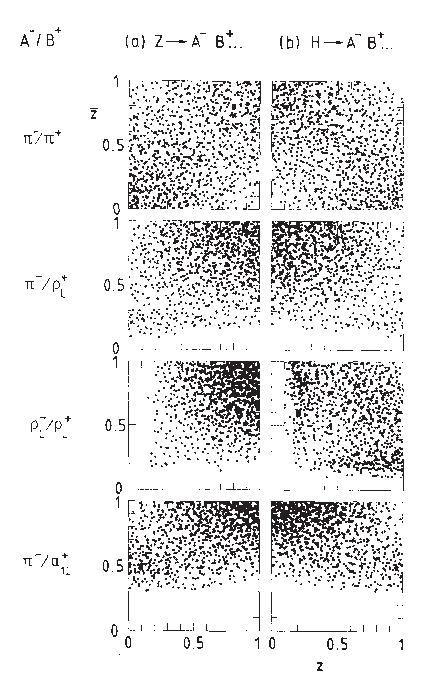
\includegraphics[width=.45\textwidth]{tau/theory}
\caption[An example of  difference in distributions for \HiggsToTauTau and \ZToTauTau.]
{
The two-dimensional distribution of (a) \HepProcess{\PZ \to \APtauon \Ptauon \to A^- B^+ \Pnut \APnut } (b) \HepProcess{\PHiggs \to \APtauon \Ptauon \to A^- B^+ \Pnut \APnut } events shown as functions of the energy fractions of $z = E_{A} / E_{\Ptauon}$ and $\overline{z} =  E_{B} / E_{\APtauon}$. In descending order the four sets of plots are for the (\APtauon, \Ptauon) pair decaying into (\Ppiminus, \Ppiplus), (\Ppiminus, $\rho_L^+$), ($\rho_L^-$, $\rho_L^+$) and finally (\Ppiminus, $a_{1L}^+$), each together with a \Pnut \APnut neutrino-pair. Plot is taken from \cite{Bullock:1991my}.
}
\label{fig:tauTheorySpin}
\end{figure}
\end{comment}

Since the tau lepton has a very short mean decay lifetime of 290\,fs \cite{Abreu:1991jn}, only tau decay products can be detected with the calorimeters and tracking detectors. Therefore, the performance of the calorimetric and track systems determines the ability to reconstruct tau lepton decay products and classify different tau decay modes. The efficiency of tau decay mode classification can be used as a benchmark for detector performance.

The main challenge in the tau lepton decay modes  classification is to reconstruct and to separate spatially close photons. For  tau leptons with energies above tens of GeV, the visible decay products are often boosted.  Electromagnetic showers from photons from \Ppizero decays often overlap each other in the calorimeters.  Reconstructing these photons as separate entities requires good photon reconstruction. Hence the photon reconstruction algorithms described in \Chapter{chap:Photon} are used in this study.

% and a fine \ECAL spatial resolution
%Since the main difference in the topologies between some final states, for example \decayRhoFinalState and \decayAiPhoton final states,  is the number of photons from \Ppizero in the final state, the ability to reconstruct the photon pairs from \Ppizero as separate particles is crucial to differentiate tau decay modes.




%Many final states of the tau decay involves \Ppizero, where \HepProcess{\Ppizero \to \Pphoton \Pphoton}.

%This chapter is organised as follows. Firstly, the choice of samples for the analysis will be discussed. The tau decay modes of interests are identified. The pre-selection cuts and variables used in the MVA classification are then discussed. The performance of the tau decay mode classification will be given, followed by an \ECAL optimisation study using the developed tau decay mode classification. Lastly, the  tau decay mode classification is further used in a proof-of-principle analysis to demonstrate the ability to identify Higgs boson from \PZ  boson using the tau pair decay channel.

%
%The impact of the \ECAL transverse spatial resolution on the tau decay classification is demonstrated as well.

This chapter presents a study of the tau decay modes classification. The ability to classify tau decay modes in a highly granular linear collider detector is used for the \ECAL optimisation study, where the impact of  the \ECAL cell sizes,  as well as the tau lepton energy, is examined.

\begin{comment}
\section{Overview of the chapter}

The analysis starts with defining samples in \Section{sec:tauDecayModes}. Seven major tau lepton decay modes are chosen for the tau decay mode classification. The simulation of these tau lepton decays is described in \Section{sec:tauSim}.  The reconstruction of the event, including the reconstruction of the invariant mass resonance for \decayRho and \decayAi decay modes, is discussed in \Section{sec:tauReco}.  After defining discriminative variables used in the MVA classification in \Section{sec:tauVar}, the classification is performed with a multivariate classifier. Since the decay products of a tau lepton need to be classified into one of the seven decay modes, a multiple class classification, presented in \Section{sec:tauMVA}, is used to allow simultaneous classification between  multiple decay modes. Afterwards, the performance of the classification is described in \Section{sec:tauClassificationEff}.

%Pre-selection of the events, discussed in \Section{sec:tauPreSel}, are such that events affected by the reconstruction and detector effects, which do not vary with the \ECAL cell sizes, are taken out of this analysis.

The classification of the tau lepton decay modes is used for the \ECAL optimisation study. The impact of  the \ECAL cell sizes,  as well as the tau lepton energy,  on the classification performance is studied in \Section{sec:tauECAL}.

The tau decay mode classification is then utilised in \Section{sec:tauHZ} to demonstrate the ability to separate Higgs boson from \PZ  boson using the tau pair decay channel, where both tau leptons subsequently decay   via  \tauToPion mode.

% for different energies of tau lepton decay to access the impact of the tau energy on the classification. The classification is also used to study the impact of the \ECAL cell sizes on the classification performance,  discussed in \Section{sec:tauECAL}.

% The difference in the spin of the boson reflects in the different spin correlation of the tau pair. By extracting the spin correlation, parent bosons can be separated.
%This classification is repeated for different energies of tau lepton decay to access the impact of energy on classification. The impact of the \ECAL design is studied afterwards, where the \ECAL square cell size is varied. An overall tau hadronic decay classification efficiency is constructed to allow direct and easy comparison between different detector design and different energies of the tau decay.

% The study of the tau final state classification in the context for the  \ECAL optimisation allows the analysis to discard reconstruction and detector issue that do not vary with the \ECAL design. For example, the early photon conversion that happens in the tracking detector would complicate the event topology. But since it is affected by the tracker design, it can be ignored in this analysis. \SECTION{sec:tauSim}  and \Section{sec:tauPreSel} discuss the pre-selection cuts to choose the signal samples and events for this analysis.

%The classification is performed with a multivariate classifier. Discriminating variables are calculated before feeding into the classifier.  A \multiclass classicisation is used to allow simultaneous classification between  multiple final states, described in \Section{}.


%A proof-of-principle analysis to demonstrate the ability to identify \PHiggs from \PZ using  tau pair decay channel is presented in the \Section{}. The difference in the spin of the boson reflects in the different spin correlation of the tau pair. By extracting the spin correlation, parent bosons can be separated.

%The follow sections on the analysis use the a 50\,GeV tau lepton decaying sample, reconstructed with nominal the \ILD detector model.
\end{comment}

\section{Event generation and simulation}
\label{sec:tauDecayModes}

%\section{Select single tau decay}  in a \ee collider for an electron-positron collider The studied tau lepton decay channel is \eeToTauTau, with a centre-of-mass energy of 100\,GeV.   predominant effect of the tau lepton decays,

Two million \eeToTauTau events at a centre-of-mass energy of 100\,GeV were generated with the \WHIZARD software \cite{whizard}.  The \TAUOLA software \cite{Jadach:1993hs} was used to describe the tau lepton decay with correct spin correlations of the tau decay products. The study is focused on separating tau decay modes. Hence the beam specific effects are not generated, such as the initial state radiation and the beam induced background. The \eeToTauTau events were simulated using the \ILD detector model as described in \Chapter{chap:Reconstruction}.




\section{Event reconstruction}
\label{sec:tauReco}

Events are reconstructed with  \ilcsoft version v01-17-07 \cite{Gaede:82475} and \pandora version 3 \cite{Marshall:2015rfa}, using the photon reconstruction discussed in \Chapter{chap:Photon}. An event display of \eeToTauTau interaction reconstructed in the \ILD detector is shown in \Figure{fig:tauEvtDsp}. The top half of the event shows a tau lepton decaying into a \decayRhoFinalState final state. The bottom half of the event shows a tau lepton decaying into a \decayThreePionPhoton final state. Purple lines represent \Ppipm tracks of the tracking detectors. Purple dots represent  calorimeter hits of the hadronic showers of \Ppipm in the \ECAL and the \HCAL. Yellow dots represent calorimeter hits of EM showers of photons  from \HepProcess{\Ppizero \to \Pphoton \Pphoton}. The blue region is the transverse cross section of the \ECAL barrel part.


%As the study is aimed for optimisation study of the \ECAL cell sizes, t

\begin{figure}[!tbph]
\centering
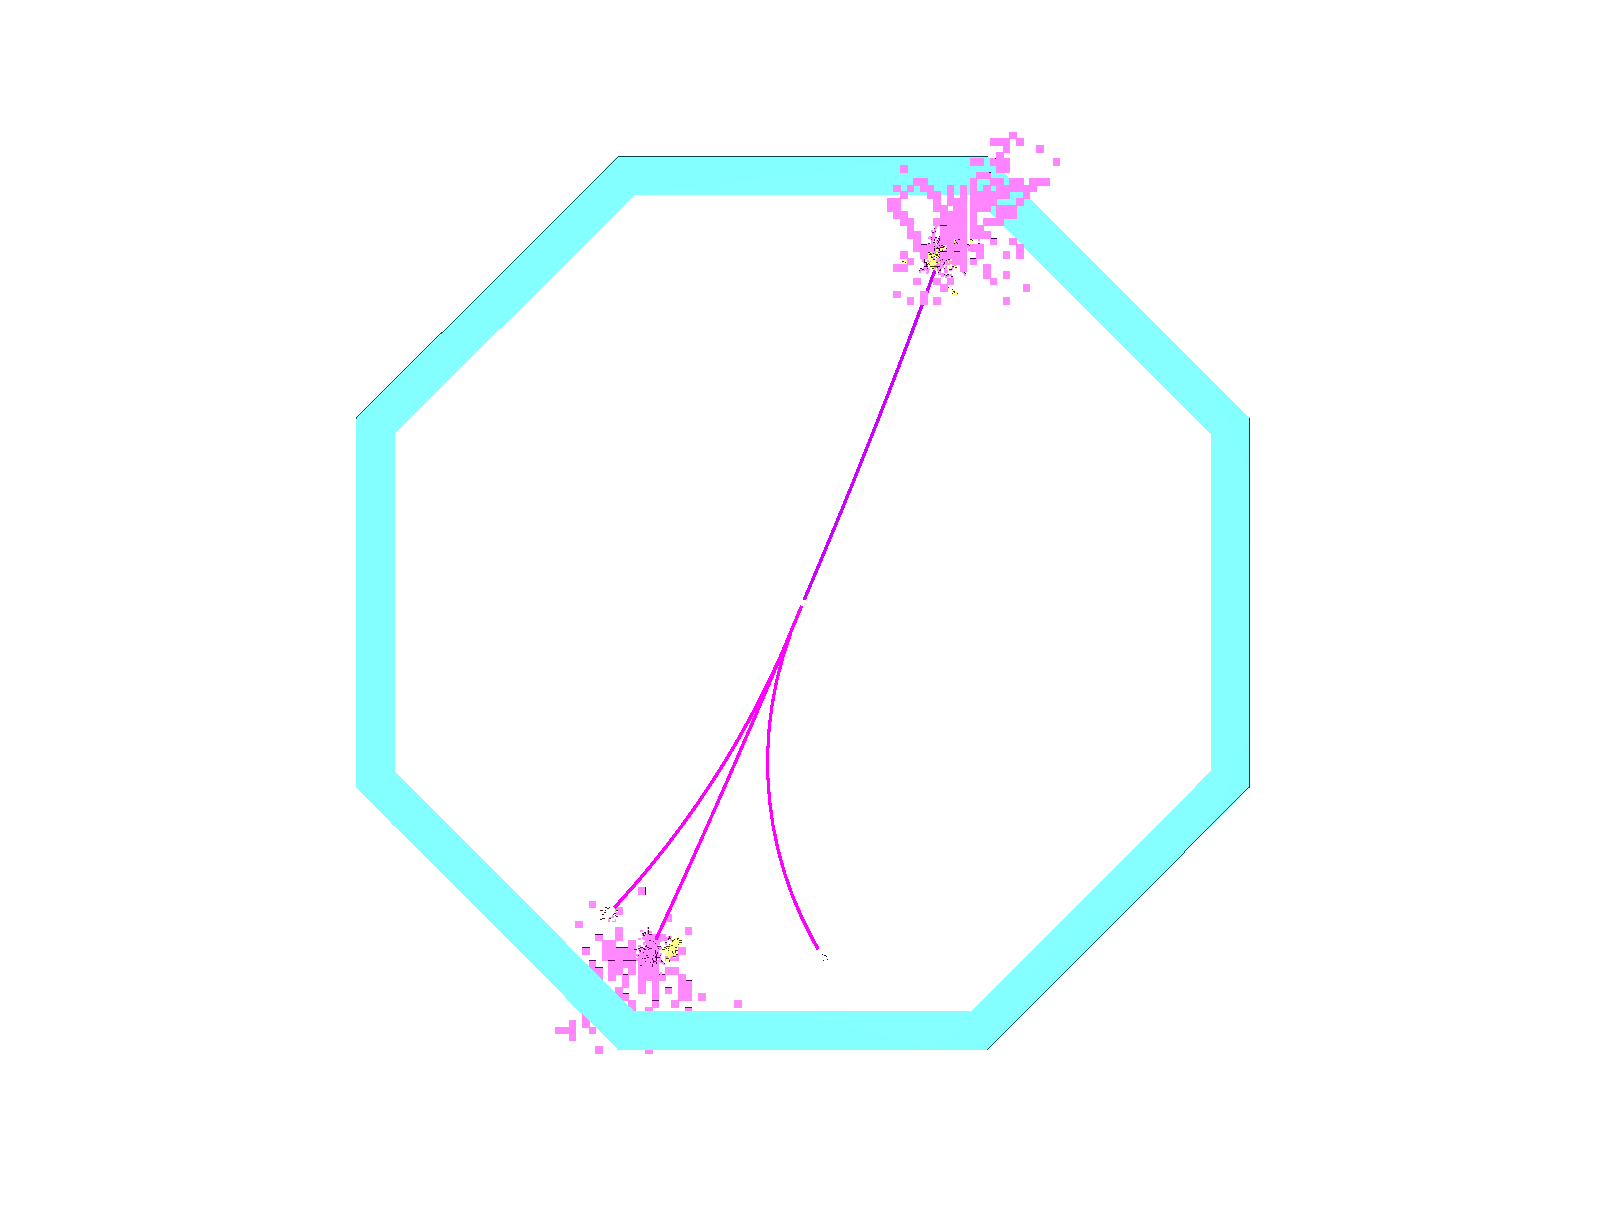
\includegraphics[width=1\textwidth]{tau/tau_evt_dsp2}
\caption{ An event display of a simulated \eeToTauTau event using the \ILD detector model. The top half of the event shows a tau lepton decaying into a \decayRhoFinalState final state. The bottom half of the event shows a tau lepton decaying into a \decayThreePionPhoton final state. Purple lines represent \Ppipm tracks of the tracking detectors. Purple dots represent  calorimeter hits of the hadronic showers of \Ppipm in the \ECAL and the \HCAL. Yellow dots represent calorimeter hits of EM showers of photons  from \HepProcess{\Ppizero \to \Pphoton \Pphoton}. The blue region is the transverse cross section of the \ECAL barrel part.}
\label{fig:tauEvtDsp}
\end{figure}




\subsection{Tau major decay modes}

To study the main decay modes of the tau lepton, decay modes with branching ratio above 2\% are classified. This results in seven tau lepton decay modes, which cover 92.58\,\% of the tau decay \cite{Agashe:2014kda}. The seven tau decay modes, their branching ratios, and detectable final states are  shown in \Table{tab:TauDecayMode}.


In the  \decayRho decay mode, the \Prho meson subsequently decays into  \decayRhoFinalStateShort. In the \decayAi  neutral and charged decay modes, the \Pai meson subsequently decays into \decayAiPhotonFinalStateShort, and \decayAiPionFinalStateShort, respectively. The invariant masses of the \Prho meson and \Pai meson are \uprightMath{775.11\pm0.34}\,MeV and \uprightMath{1230\pm40}\,MeV, respectively \cite{Agashe:2014kda}.

%Thrust axis is useful to separate each jet in a back-to-back two-jet event.
%Thrust value, $T$, is 1 for a perfect pencillike back-to-back two-jet event, and 0.5 for a perfect spherical event. The thrust value is useful in picking out back-to-back two-jet event.


%\subsection{Tau lepton decay modes}

%Tau lepton decays into a number of final states.
% The most difficult final states to separate are \decayRhoFinalStateShort and \decayAiPhotonFinalStateShort, where photons from boosted \Ppizero are very challenging to reconstruct correctly.

\begin{table}[htbp]\centering
\smallskip
\begin{tabular}{l l r}
\hline
\hline
Decay mode  & Detectable final state & Branching ratio\\
\hline
\decayElectron   &  \decayElectronShort  & $17.83{\pm0.04\%}$   \\
\decayMuon &	\decayMuonShort & $17.41{\pm0.04\%}$  \\
\decayPion  &   \decayPionShort	& $10.83{\pm0.06\%}$   \\
\decayRho   & \decayRhoFinalStateShort& $25.52{\pm0.09\%}$ \\
\decayAi neutral  & \decayAiPhotonFinalStateShort	& $9.30{\pm0.11\%}$    \\
\decayAi charged &	\decayAiPionFinalStateShort    & $8.99{\pm0.06\%}$  \\
\decayThreePionPhoton  &	\decayThreePionPhotonShort    & $2.70{\pm0.08\%}$  \\
\hline
\hline
\end{tabular}
\caption[Decay modes, detectable final state particles and branching ratios of the seven major \Pgtm decays.]
{Decay modes, detectable final state particles, and branching ratios of seven major \Pgtm decay modes. Values are taken from \cite{Agashe:2014kda}.}
\label{tab:TauDecayMode}
\end{table}


\subsection{Selecting single tau decay}

The \eeToTauTau channel contains two tau leptons. Since the tau decay mode classification is applied on a per-tau-lepton basis, the decay products of the two tau leptons in one event are divided into two sets for individual tau decay mode classifications. By identifying the axis of the back-to-back taus in the  \eeToTauTau event, the detector space can be separated in two hemispheres, where particles in each hemisphere correspond to the decay products of one tau lepton.

Separating reconstructed particles in an event into two sets is achieved using the principle thrust axis vector of the event, which is the axis that most particle are aligned to. The principle thrust axis vector, $\hat{t}$, is determined by maximising the thrust \cite{PhysRevLett.39.1587}, $T$:
\begin{equation}
T = \max_{\hat{t}}\!\frac{\sum_{i}\absOf{\hat{t}\!\cdot\!\vec{p_{i}}}}{\sum_{i}\absOf{\vec{p_{i}}}},
\end{equation}
where $\vec{p_{i}}$ is the momentum vector of particle $i$;  vector $\hat{t}$ is the unit principle thrust axis vector; and index $i$ is summed over all particles in an event. Two sets of particles are obtained based on the sign of the scalar product between the principle thrust axis vector  and the momentum vector of a particle: particles with a positive sign of the scalar products are in one set and particles with a negative sign are in another set.


\section{Pre-selection}

Three pre-selection cuts are used based on the MC information of the particles. The cuts and the number of tau decays passing the cuts are listed in \Table{tab:tauPreSelEff}.

Since this study is focused on the photon reconstruction in the \ECAL to classify tau decay modes, the tau decay products with photon conversion to electron pairs in the tracking detector are not considered.

Another pre-selection cut requires the total visible energy (i.e. not accounting for neutrinos) of tau decay products, $E_{vis,MC}$, to be greater than 5\,GeV.

Lastly, tay decay products are discarded when tau decay products deposit energies in the gap region between barrel and  endcap part of the calorimeter, because there is a degradation in the particle reconstruction efficiency in the gap region. Tau decay products with the generated polar angle of the tau lepton in the region of 0.6\,rad and 0.9\,rad are not considered.

%The cut demands the absolute value of the generated polar angle of the tau lepton with respect to the beam direction, $\absOf{\theta_{Z,MC}}$, is between 0.3\,rad and 0.6\,rad to be  in the endcap region, or is between 0.8\,rad and $\frac{\pi}{2}$\,rad to be  in the barrel region.


%Simulated events are further constrained to focus on the events with clear topologies, based on the truth information. The constraints on the samples are

%Three sets of constraints are used. One set of constraints is that events are discarded when photons in the tau decay products convert to electron pairs in the tracking detector. Since the reconstruction does not attempt to recover photons from electron pairs, these events would have a fewer number of photons reconstructed than expected.


%.  Since the reconstruction does not attempt to recover photons from electron pairs, events with converted photons are discarded.

%, which changes the topologies of the final states.

%Another set of constraints requires the total energy of the non-neutrino tau decay products, $E_{vis,MC}$, to be greater than 5\,GeV. If most energy of a tau lepton is carried by  neutrinos, non-neutrino decay products would have low energies and be difficult to be reconstructed.

%Hence these events with low-energy non-neutrinos tau decay products are not used in the analysis.



%Last set of constraints requires events to be discarded when tau decay products deposit energies in the gap region between barrel and  endcap part of the calorimeter. As the reconstruction   does not attempt to recover reconstruction in the gap region, there is a degradation in the particle reconstruction efficiency in the gap region. The constraint demands the absolute value of the polar angle of tau lepton with respect to the beam direction, $\absOf{\theta_{Z,MC}}$, is between 0.3\,rad and 0.6\,rad to be  in the endcap region, or is between 0.8\,rad and $\frac{\pi}{2}$\,rad to be  in the barrel region.

\TABLE{tab:tauPreSelEff} shows the fractions of tau decays passing successive cuts  for different tau decay final states.  As expected, the cut on the photon conversion only affects tau decay modes with  photons in the final states. The cut on the total visible energy of the tau decay products has the greatest affect on the leptonic decay modes with two neutrinos  in the final states. The cut on the tau polar angle affects different tau decay modes almost equally.

% because more energies are carried by neutrinos in these decay modes.

%All decay modes are affected almost equally by this cut, suggested by numbers in \Table{tab:tauPreSelEff}.



\begin{table}[htbp]\centering
\smallskip
\begin{tabular}{ l r r r}
\hline
\hline
 \multicolumn{1}{L{0.2\textwidth}}{Detectable final state}   & \multicolumn{1}{R{0.2\textwidth}}{No photon conversion} & \multicolumn{1}{R{0.2\textwidth}}{$E_{vis,MC}$ > 5\,GeV} &\multicolumn{1}{R{0.2\textwidth}}{$\absOf{\theta_{Z,MC}}$} \\
\hline
\decayElectronShort& 100.0\% & 84.7\%& 66.2\%\\
\decayMuonShort &100.0\%& 85.2\%&66.7\%\\
\decayPionShort &100.0\%& 88.3\%&60.9\%\\
\decayRhoFinalStateShort &77.1\%&76.9\%&61.9\%\\
\decayAiPhotonFinalStateShort &61.3\%&61.2\%&50.5\%\\
\decayAiPionFinalStateShort &100.0\%&100.0\%&78.0\%\\
\decayThreePionPhotonShort &77.0\%&77.0\%&61.8\%\\
\hline
\hline
\end{tabular}
\caption
{Fractions of tau decays passing successive pre-selection cuts  for different tau decay final states.}%All cuts are based on the truth information.
\label{tab:tauPreSelEff}
\end{table}

\begin{comment}
\section{Event simulation}
\label{sec:tauSim}


The \eeToTauTau events were simulated using the \ILD detector model. The software used for simulation is described in \Chapter{chap:Reconstruction}.

%that are not affected by the varying \ECAL cell sizes
The beam specific effects are not simulated, such as the initial state radiation and the beam induced background, as the analysis is optimised for the use of the \ECAL optimisation study.





\begin{table}[htbp]\centering
\smallskip
\begin{tabular}{l r}
\hline
\hline
Cuts & Values\\
\hline
\multicolumn{1}{L{0.4\textwidth}}{Photon conversion in the tracking detector}& No \\
\multicolumn{1}{L{0.4\textwidth}}{Total energy of non-neutrino decay products} & $E_{vis,MC} > 5\,GeV$ \\
Polar angle acceptance & \multicolumn{1}{R{0.5\textwidth}}{$0.6 > \absOf{\theta_{Z,MC}} > 0.3$ or $1.57 > \absOf{\theta_{Z,MC}} > 0.8$} \\
\hline
\hline
\end{tabular}
\caption[Pre-selection cuts for tau lepton decay final state classification.]
{Pre-selection cuts for tau lepton decay modes classification.}
\label{tab:tauPreSel}
\end{table}

\section{Event pre-selection}
\label{sec:tauPreSel}

Pre-selection cuts select events using the truth information. Since the analysis is aimed for the optimisation of the \ECAL cell sizes, these pre-selection cuts are such that effects not affected by the changing of the \ECAL cell sizes are not considered in the analysis. These cuts allow the analysis to focus on the events with clear topologies. The pre-selection cuts are listed in \Table{tab:tauPreSel}. The fraction of events passing each pre-selection cut for individual decay mode are listed in \Table{tab:tauPreSelEff}.

One of the pre-selection cuts is to demand that the tau decay products  do not have photons converted to electron pairs in the tracking detector, determined with the truth information. These discarded events would have fewer photons and more electrons than expected in the final states, which changes the topologies of the final states. Shown in \Table{tab:tauPreSelEff}, only decay modes with photons in the final states are affected by this cut, as expected.


Another pre-selection cut requires the total energy of the non-neutrino tau decay products, $E_{vis,MC}$, to be greater than 5\,GeV, based on the truth information. If most energy of a tau lepton is carried by  neutrinos, non-neutrino decay products would have low energies and be difficult to be identified. Hence these events with low-energy non-neutrinos tau decay products are not used in the analysis. Decay modes with only one non-neutrino particle in the final states are mostly affected by this cut because more energies are carried by neutrinos, indicated in \Table{tab:tauPreSelEff}.

The last pre-selection cut is to discard events with tau decay products depositing energies in the gap region between barrel and the end cap part of the calorimeter. As the reconstruction   does not attempt to recover reconstruction in the gap region, there is a significant drop in the particle reconstruction efficiency in the gap region. The cut demands the absolute value of the polar angle of tau lepton, based on the truth information, $\absOf{\theta_{Z,MC}}$, is between 0.3 and 0.6\,rad to be contained in the end cap region, or is between 0.8 and 1.57\,rad to be contained in the barrel region. All decay modes are affected almost equally by this cut, suggested by numbers in \Table{tab:tauPreSelEff}.

\end{comment}

%The no photon early conversion cuts only effective against final states with \Ppizero, as \Ppizero decays to a photon pair. For final states with one \Ppizero, about 77\% events survived. For final states with two \Ppizero, about 61\% events survived, which is roughly $0.77^2$. For the visible angle acceptance, final states with only one particle are affected the most, whilst final states with more than one particles typically have more visible energies. The polar angle acceptance efficiencies depend on the final states, as light final states are boosted and more likely in the forward region.



%An low visible energy event is discarded if the total energy of the tau lepton visible decay products is below 5\,GeV. Requirement of the tau decay in the barrel or the end cap part of the calorimeter is defined as the polar angle of the tau is $ 17.2\degree < |\theta_{Z}| < 34.4\degree$ or $ 45.8\degree < |\theta_{Z}| < 90\degree$.



\section{Variables used in MVA}
\label{sec:tauVar}

The classification of different tau decays uses a MVA classification based on twenty seven discriminant variables. These are listed in \Table{tab:tauVaraibles}. The particle ID information comes from the output of the \pandora reconstruction.

%After event reconstruction,  27 discriminative variables used in the MVA  classification  are  developed and listed in \Table{tab:tauVaraibles}. The distributions of four powerful variables for different tau decay modes are shown in \Figure{fig:tauVar}.

%Having pre-selected events,  variables are carefully developed for the multivariate analysis (MVA). The full list of the variables are shown in \Table{tab:tauVaraibles}.

\begin{table}[!htbp]\centering
\begin{tabular}{lr}
\hline
\hline
Category &  Variable \\
\hline
Particle numbers  &{  ${N}_{\charge}$, ${N}_{\Pmu}$, ${N}_{\Pe}$, ${N}_{\Pgg}$,  ${N}_{\Pgpm}$} \\
Invariant masses & {$m_{vis}$, $m_{\charge}$, $m_{\neutral}$, $m_{\Pgg}$, $m_{\Pgpm}$} \\
Energy variables & { $\tilde{E}_{vis}$,  $\tilde{E}_{\charge}$, $\tilde{E}_{\Pmu}$, $\tilde{E}_{\Pe}$, $\tilde{E}_{\Pgg}$,  $\tilde{E}_{\Pgpm}$} \\
Calorimetric energy information &   { $E^{\ECAL}_{\charge} / E_{\charge}$,  $ E^{\ECAL} / E$ } \\
\decayRhoShort reconstruction &{  $m_{\Pgpz}^{\parenths{\Prho}}$, $m_{\Prho}^{reco}$} \\
\decayAiPhotonShort reconstruction & {  $m_{\Pgpz}^{(\Pai)}$, $m^{*(\Pai)}_{\Pgpz}$, $m_{\Pai}^{reco}$} \\
EM shower profile & $\delta{l}$, $t_0$, $\langle{w}\rangle$ \\
Calorimeter hit information & $\bar{E}_{hit}$, $MIP$ \\
Track information & $E/p$ \\
\hline
\hline
\end{tabular}
\caption
{Variables used in the MVA classification for the tau lepton decay mode classification.}
\label{tab:tauVaraibles}
\end{table}

\subsection{Particle number variables}

The most crucial variables for classifying tau decay modes  are the number of particle of different types of particles. There are five variables used in the MVA classification: the number of charged particles (${N}_{\charge}$); the number of muons (${N}_{\Pmu}$); the number of electrons (${N}_{\Pe}$); the number of photons (${N}_{\Pgg}$); and the number of charged pions (${N}_{\Pgpm}$).



\FIGURE{fig:tauVarNCharge} shows the distribution of the number of reconstructed charged particles for different tau decay modes. Over 98\% of  \tauToElectron, \tauToMuon, and \tauToPion final state events have exactly one reconstructed charged particle  per event, and approximately 95\% of \decayAiPionShort final state events give exactly three reconstructed charged particles. \FIGURE{fig:tauVarNMuon} and \Figure{fig:tauVarNElectron}  show the distributions of the number of reconstructed muons and electrons respectively for different tau decay modes. 99\% of \tauToMuon final state events produce exactly one reconstructed muon, and 99\% of \tauToElectron final state events have one reconstructed electron. \FIGURE{fig:tauVarNPhoton} shows the distributions of the number of reconstructed photons  for different tau decay modes, which distinguishes between final states with different numbers of \Ppizero.  Nearly 75\% of  \decayRhoShort  decays give exactly two reconstructed photons, and over 60\% of the \decayAiPhotonShort decays have exactly four photons.




\begin{figure}[htbp]
\centering
% \begin{center}/\end{center} takes some additional vertical space
\begin{subfigure}[b]{0.45\textwidth}
 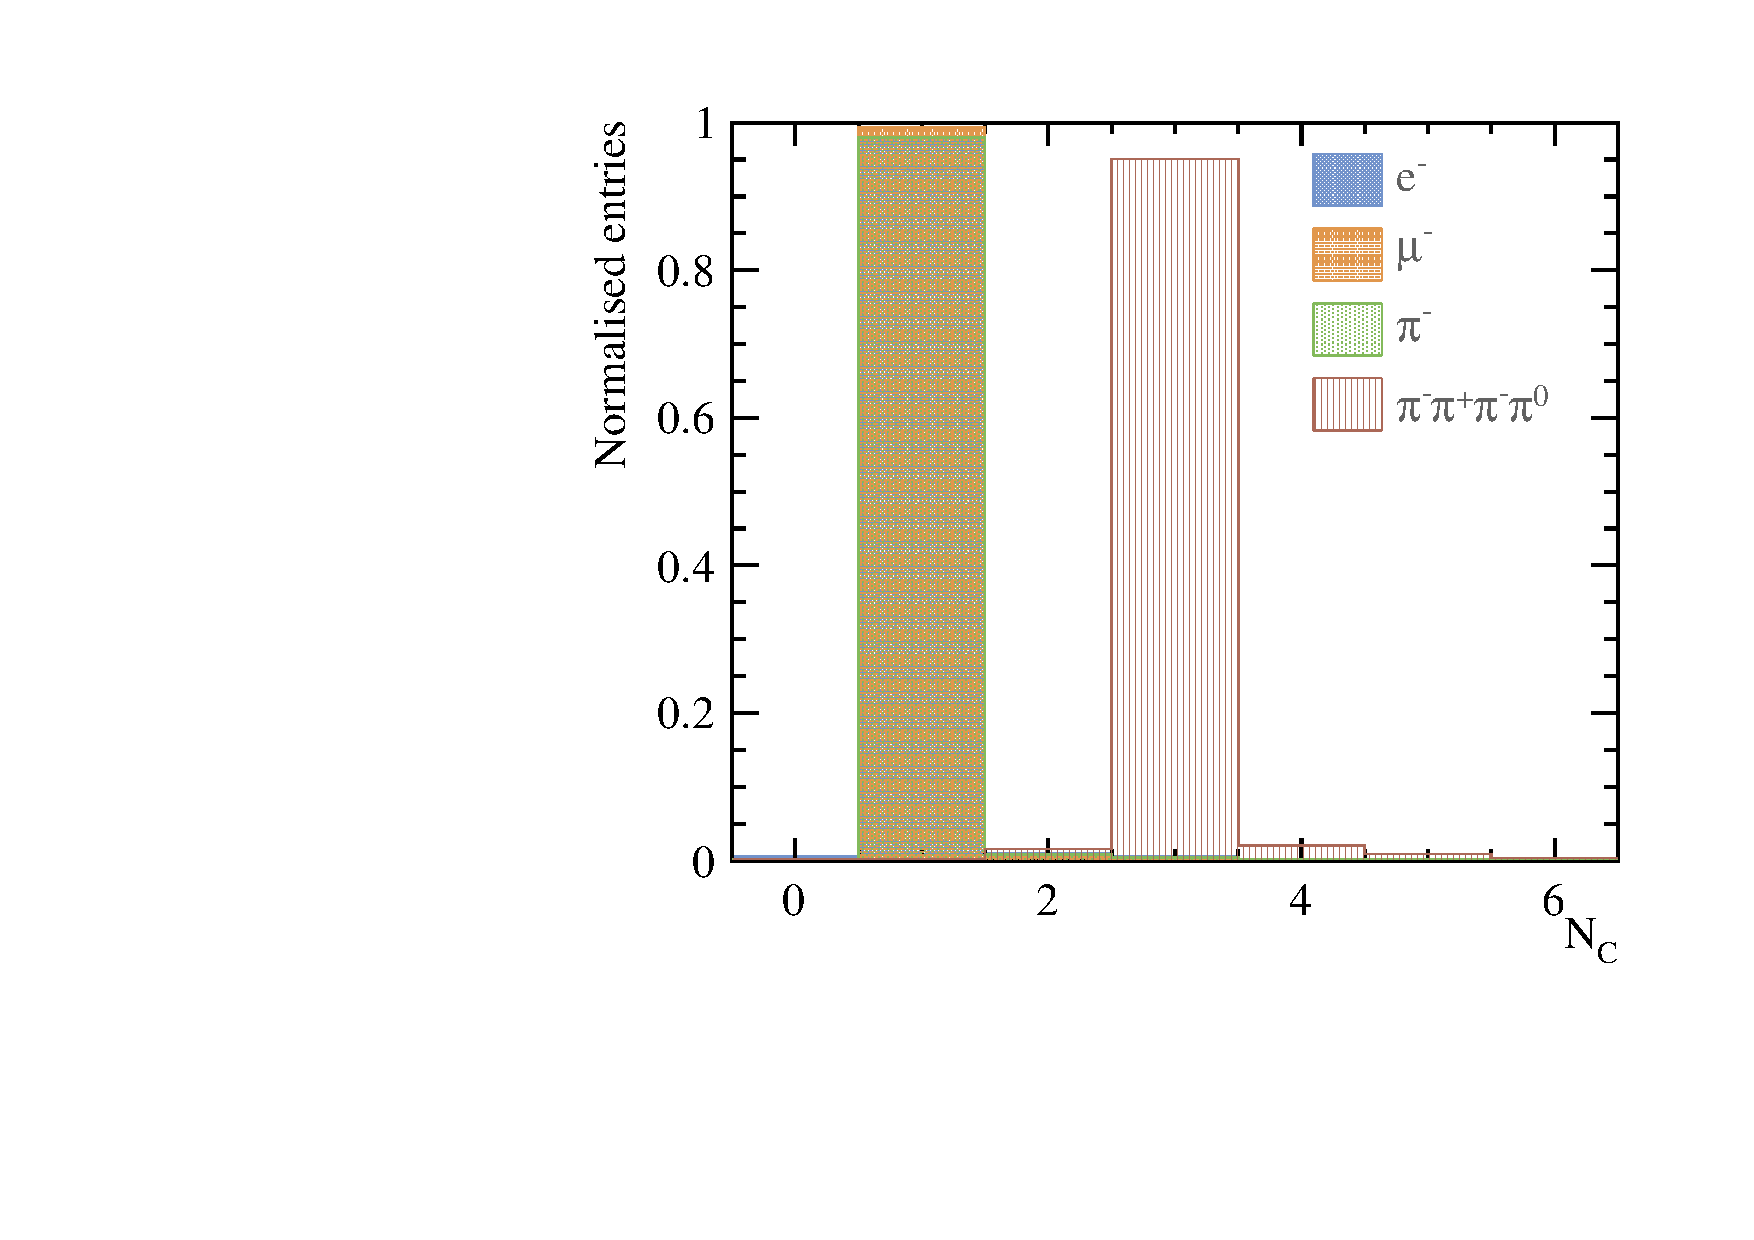
\includegraphics[width=\textwidth]{tau/nCharge_100GeV_improved.pdf}
  \caption{}
  \label{fig:tauVarNCharge}
\end{subfigure}
\begin{subfigure}[b]{0.45\textwidth}
 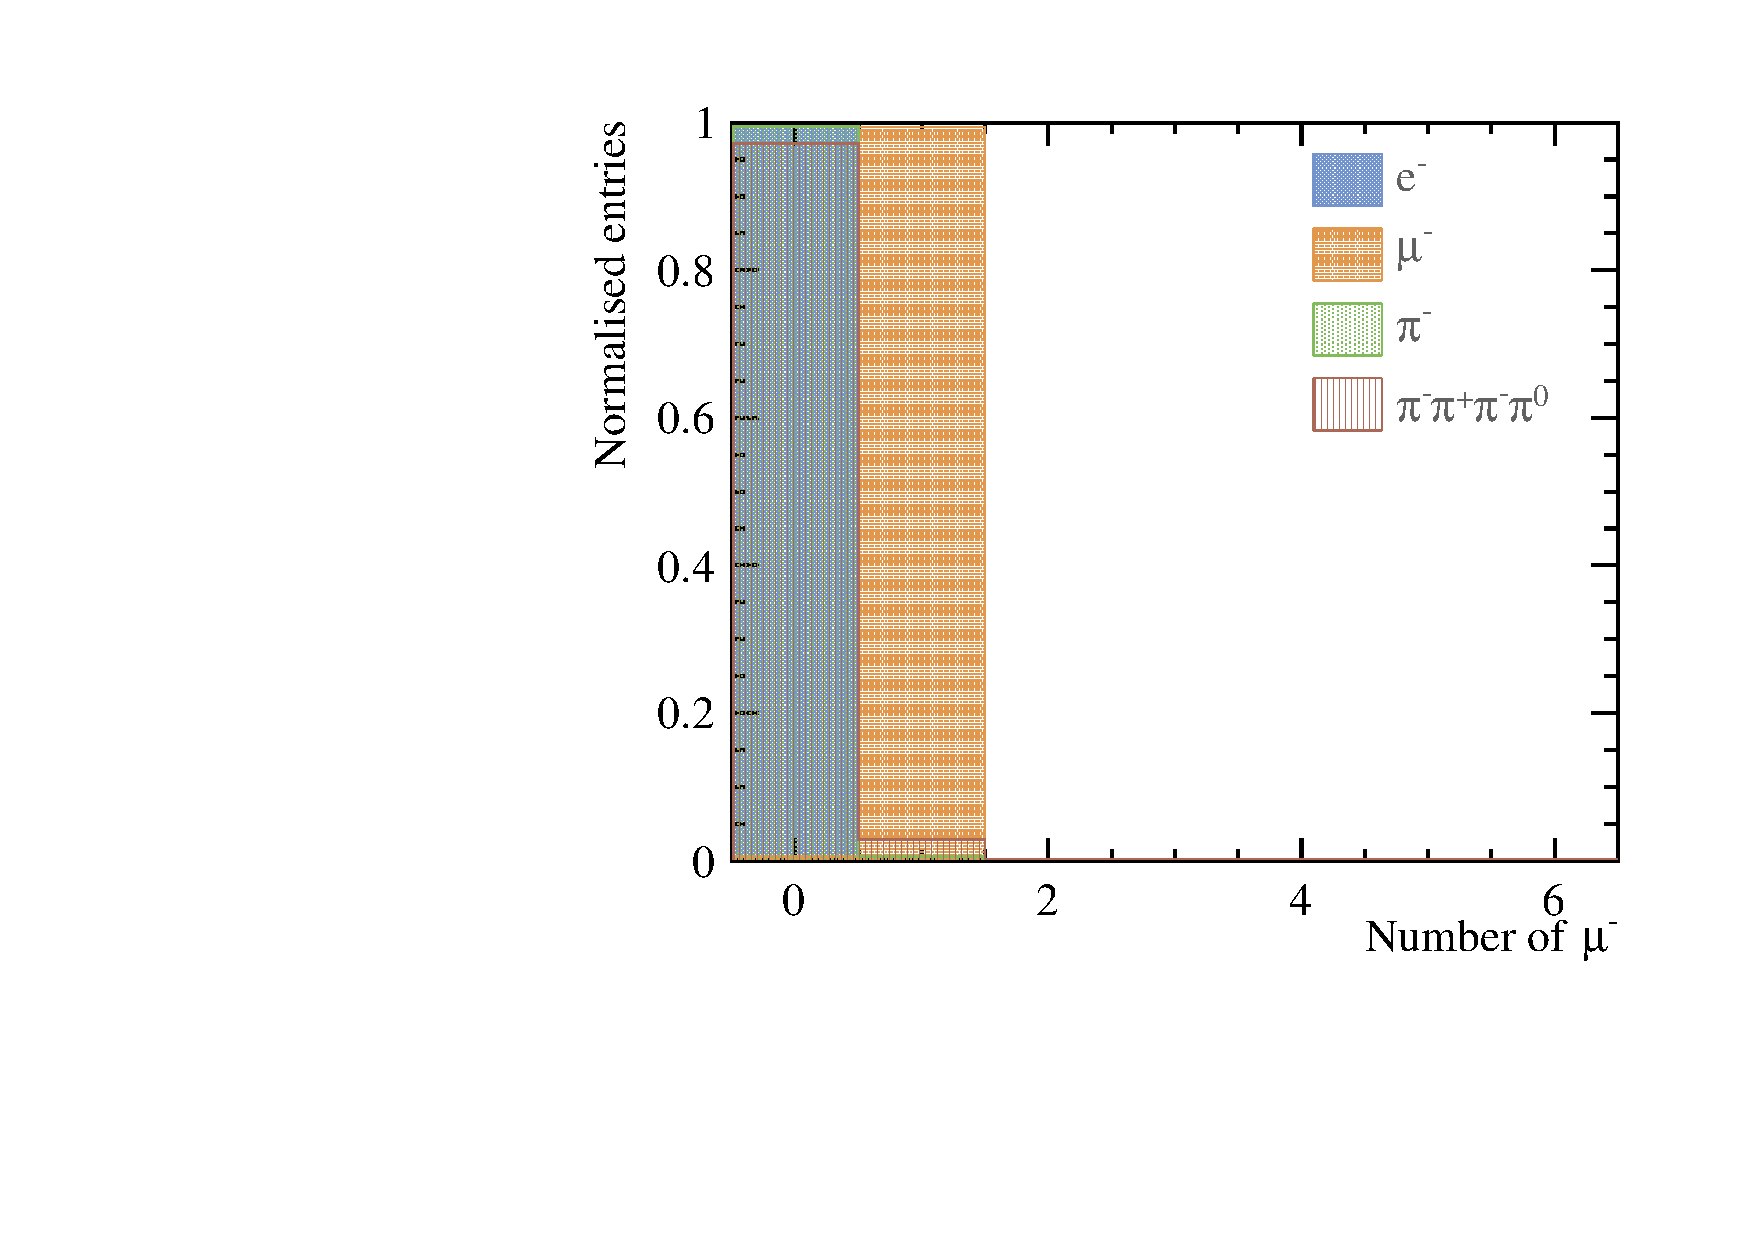
\includegraphics[width=\textwidth]{tau/nMuon_100GeV_improved.pdf}
  \caption{}
  \label{fig:tauVarNMuon}
\end{subfigure}
\begin{subfigure}[b]{0.45\textwidth}
 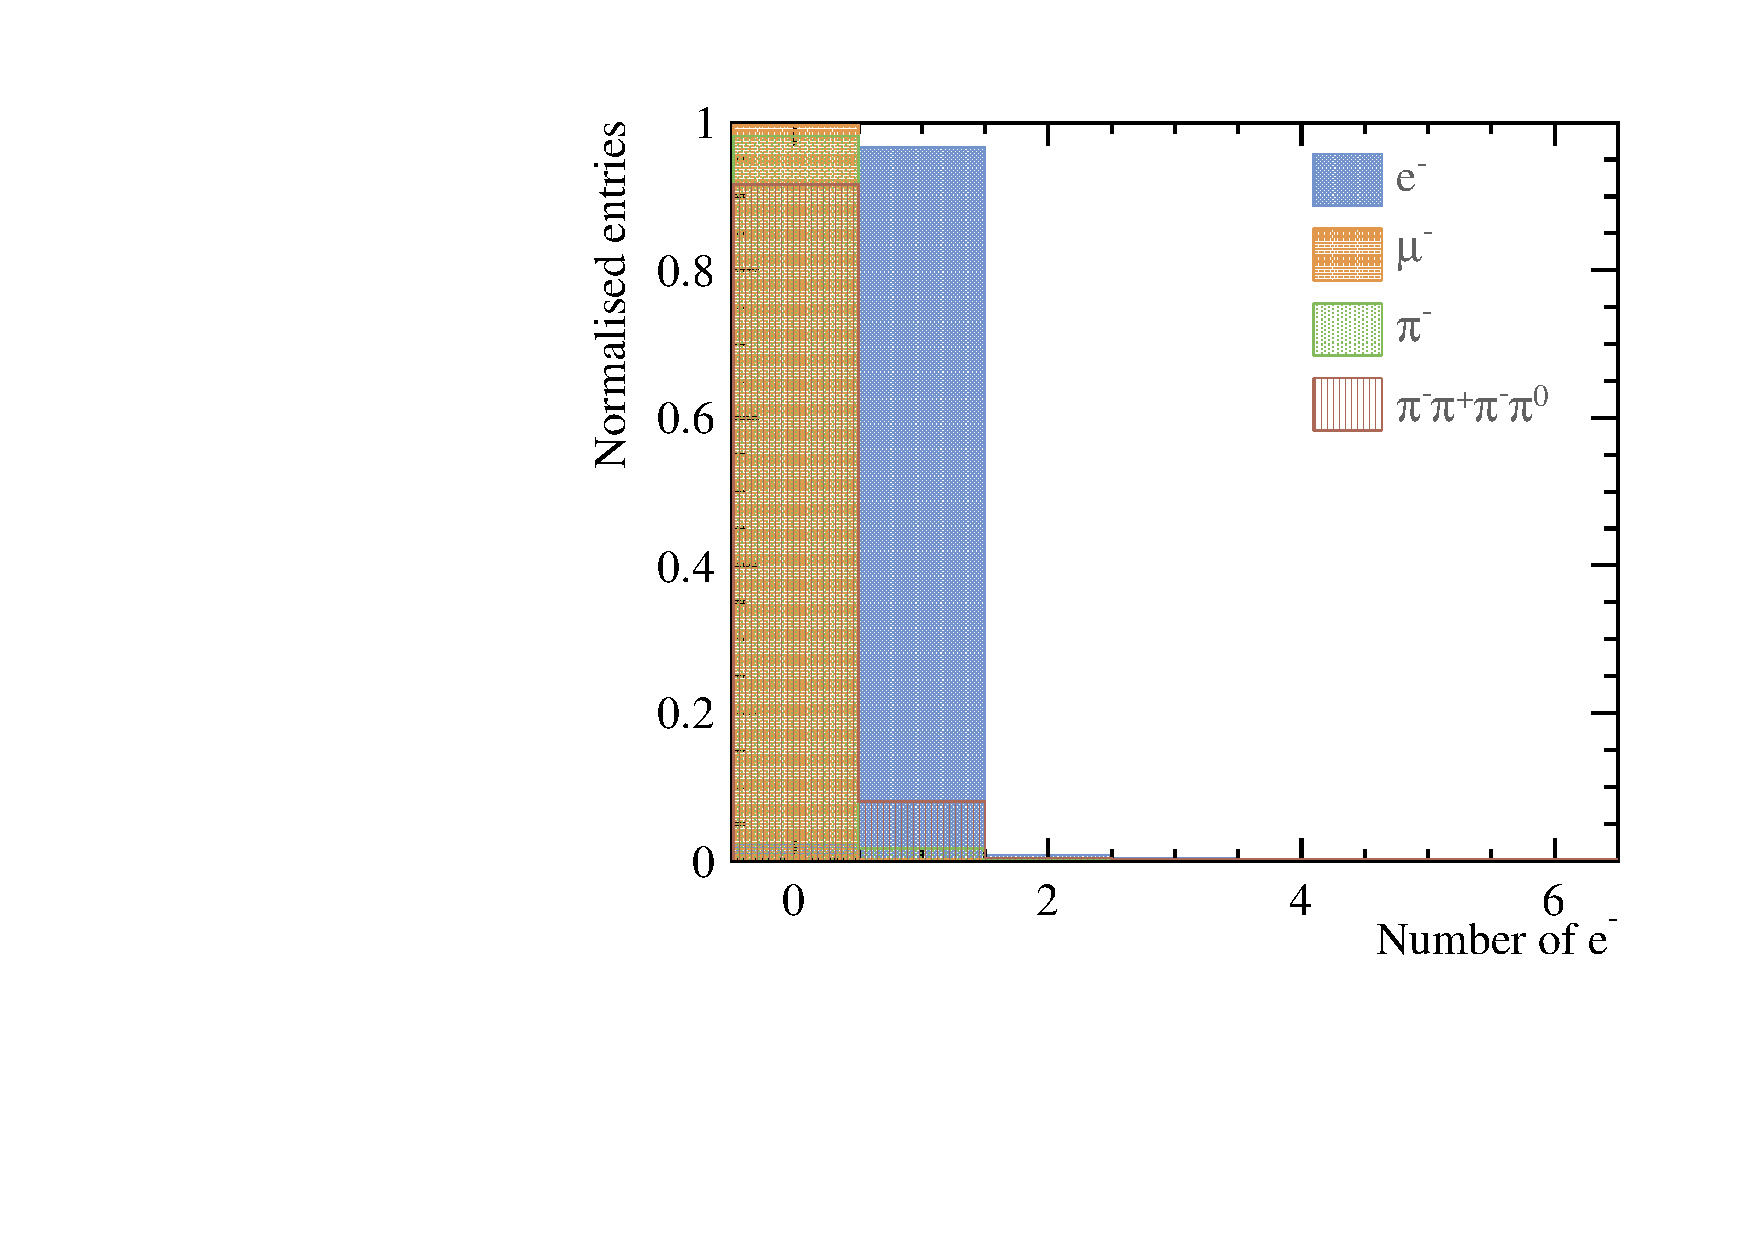
\includegraphics[width=\textwidth]{tau/nElectron_100GeV_improved.pdf}
  \caption{}
  \label{fig:tauVarNElectron}
\end{subfigure}
\begin{subfigure}[b]{0.45\textwidth}
 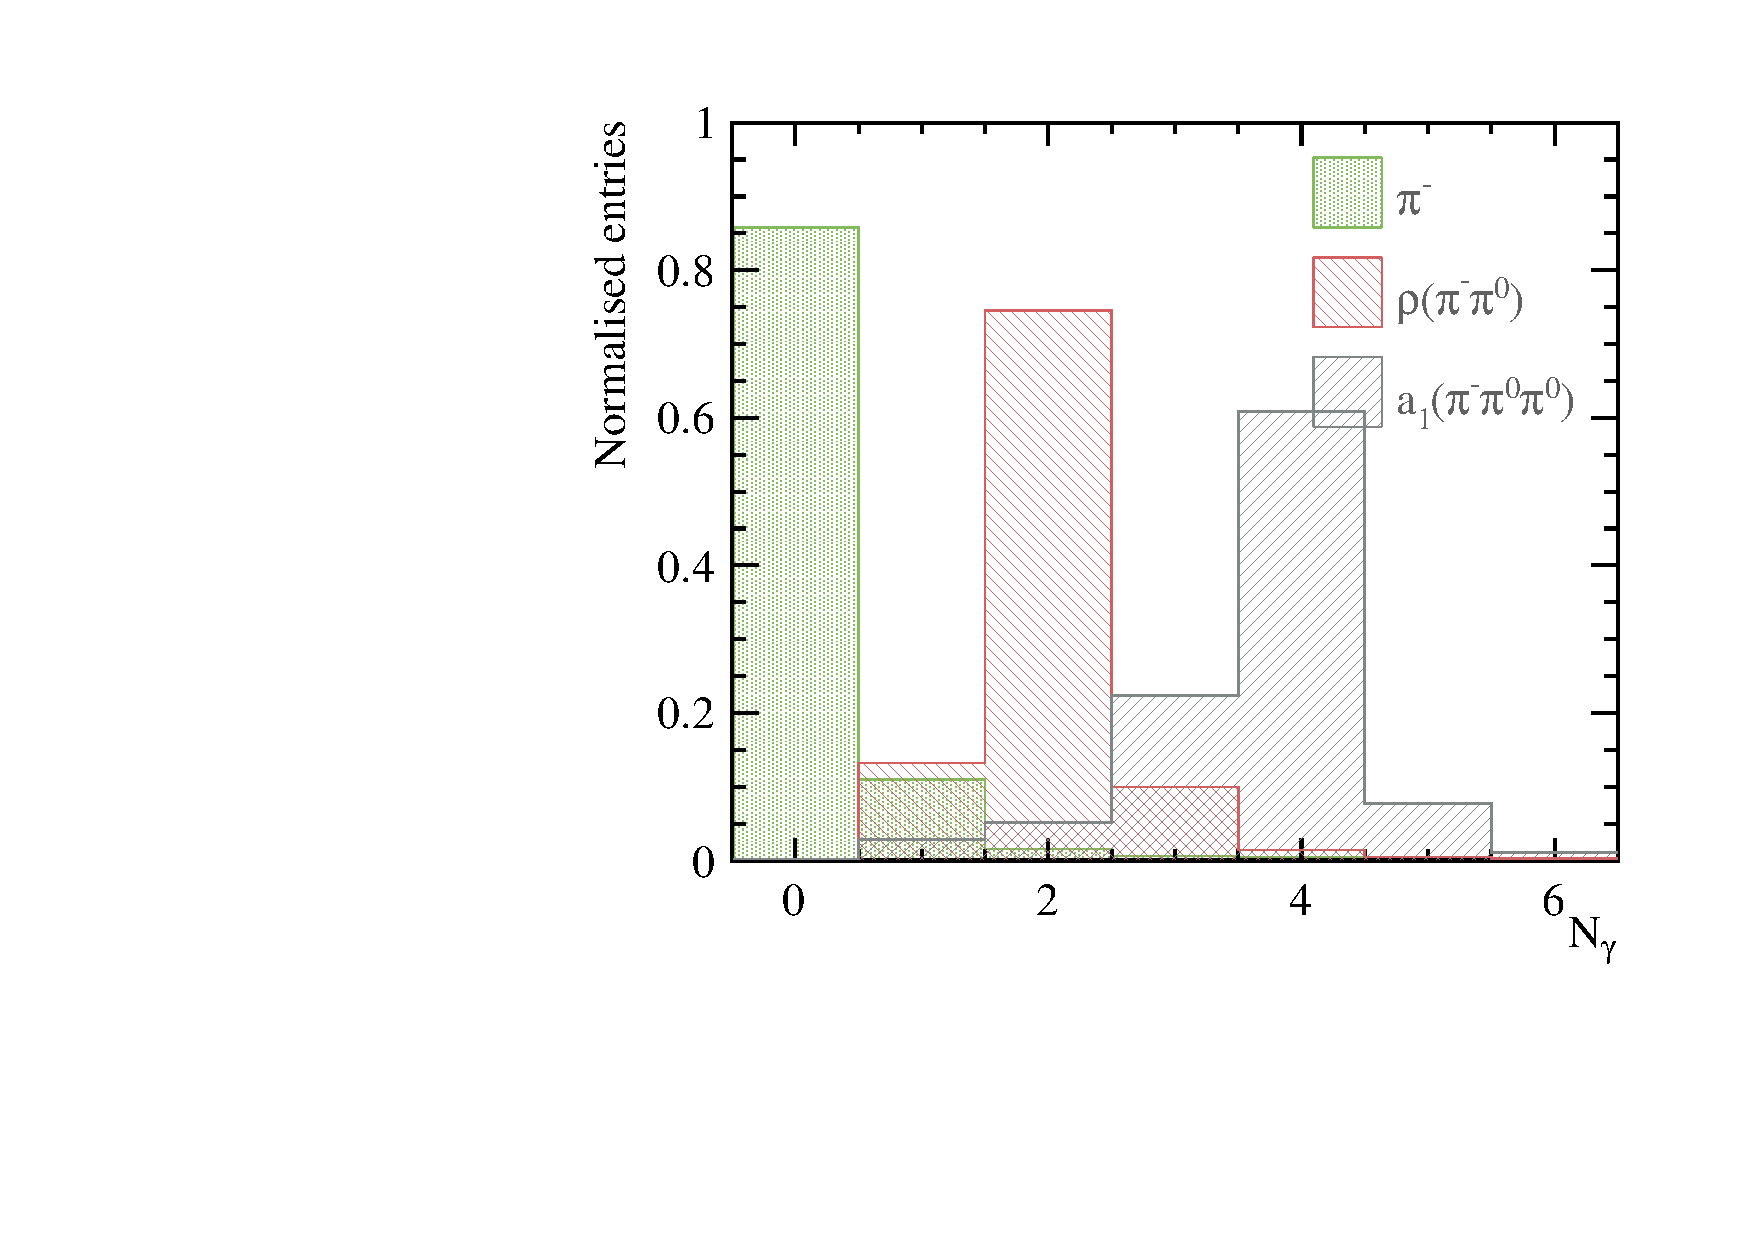
\includegraphics[width=\textwidth]{tau/var2/nPhoton_100GeV_improved.pdf}
  \caption{}
  \label{fig:tauVarNPhoton}
\end{subfigure}
\caption
{Distributions of  the number of reconstructed a)  charged particles (${N}_{\charge}$); b) muons (${N}_{\Pmu}$); c) electrons (${N}_{\Pe}$); d) and photons (${N}_{\Pgg}$). The particle ID information comes from the output of the \pandora reconstruction. The area under the curve for each decay mode is normalised to unity. Decay modes in all plots are selected using the truth information.}
\label{fig:tauVar}
\end{figure}

% and the overlap between \decayRhoShort and \decayAiPhotonShort is around 15\%. ${N}_{\Pgg}$ can also separate two 3-prong final states.
%${N}_{\Pmu}$, ${N}_{\Pe}$, ${N}_{\Pgpm}$ are useful to identify two leptonic final states, and further separate 3-prong final states from 1-prong final states.
%This is an excellent variable to separate 1-prong and 3-prong final states.  An orthogonal measurement is the number of reconstructed photons,  ${N}_{\Pgg}$, shown in \Figure{fig:tauVarNPhoton}.

\subsection{Invariant mass variables}

Five invariant mass variables participate in the MVA classification: the invariant mass of all non-neutrino decay products ($m_{vis}$); the invariant mass of all charged particles ($m_{\charge}$); the invariant mass of all neutral particles ($m_{\neutral}$); the invariant mass of all photons ($m_{\Pgg}$); and the invariant mass of all charged pions ($m_{\Pgpm}$). \FIGURE{fig:tauVarMVis} shows the distributions of the invariant mass of all non-neutrino decay products for different tau decay modes. Resonance peaks in the invariant mass distribution can be seen for \Prho and \Pai decay modes in the figure.

%Invariant masses of different particles are good at characterising different final states. \FIGURE{fig:tauVarMVis} shows the invariant mass of the system. Clear reasonable peaks can be seen for \Prho and \Pai. The mass peak of  \decayAiPionFinalStateShort are much higher. $m_{\charge}$ and $m_{\neutral}$ are invariant masses of charged and neutral particles respectively. They separate final states with neutral particles from those without neutral particles. Similarly, $m_{\Pgg}$ and $m_{\Pgpm}$ identify final states with photons and with \Pgpm respectively.

\subsection{Energy variables}

Energy information helps to further separate different tau decay modes. Six energy variables are used in the MVA classification: the normalised total energy of all non-neutrino decay products ($\tilde{E}_{vis}$); the normalised total energy of charged particles ($\tilde{E}_{\charge}$); the normalised total energy of muons ($\tilde{E}_{\Pmu}$); the normalised total energy of electrons ($\tilde{E}_{\Pe}$); the normalised total energy of photons ($\tilde{E}_{\Pgg}$); and the normalised total energy of charged pions ($\tilde{E}_{\Pgpm}$). All variables are normalised with respect to the energy of the associated tau lepton.

\subsection{Calorimetric information variables}


Two calorimetric information variable are used in the MVA classification: the fraction of the energy  deposited in the \ECAL divided by the  energy deposited in the calorimeters for all charged particles ($\% E_{\charge}$), and the fraction of the energy  deposited in the \ECAL divided by the  energy deposited in the calorimeters for all particles ($\% E$). These  two variables help to identify electron and muon decay modes. For example, an electron typically deposits over 95\% of its energy in the \ECAL, and a muon typically deposits 5\% to 20\% energy in the \ECAL. The difference between $\% E_{\charge}$ and  $\% E$ is that photons, which deposit most of their energy in the \ECAL, do not participate in the calculation of $\% E_{\charge}$.

\subsection{\texorpdfstring{\decayRhoShort and \decayAiPhotonShort} \, resonances variables}


\section{\texorpdfstring{\decayRhoShort and \decayAiPhotonShort} \, resonances reconstruction}
\label{sec:tauResonance}

By utilising the photon identification potential of the highly granular \ECAL, the identification of the \decayRhoShort and \decayAiPhotonShort decay modes is enhanced  by reconstructing the \Prho and \Pai invariant mass. For events with at least one charged pion and one photon, the reconstruction selects the combination of charged pion and photon that have a invariant mass consistent with the \Prho or \Pai mass.



%The identification of the \decayRhoShort and \decayAiPhotonShort decay modes is enhanced  by reconstructing the \Prho and \Pai invariant mass. The


%The \decayRhoShort and \decayAiPhotonShort decay modes identification is enhanced  by reconstructing the \Prho and \Pai invariant mass resonances.
% By selecting \Pgpm and photons consistent with \Prho mass, \decayRhoShort decay mode reconstruction is improved.
For example, the final state of the \decayRhoShort decay mode contains a \Pgpm and a \Ppizero, where  \pionToPhoton. The  \decayRhoShort decay mode hypothesis test is performed by selecting the combination of the charged pion and photons that gives the smallest value of a $\chi^{2}$ function:
\begin{equation}
\chi^{2} = {\left(\frac{m_{tot} -  m_{\Prho}}{\sigma_{\Prho}}\right)}^{2} + {\left(\frac{m_{\Pphoton_1\Pphoton_2} -  m_{\Ppizero}}{\sigma_{\Ppizero}}\right)}^{2} \,,
\label{eqn:tauRho}
\end{equation}
where $m_{\Pphoton_1\Pphoton_2}$ is the invariant mass of two photons; the variable $m_{tot}$ is the total invariant mass of the  two photons and one \Pgpm; the variables $m_{\Prho}$ and $m_{\Ppizero}$ are the respective true masses of \Prho and \Ppizero, taken from \cite{Agashe:2014kda}; and the mass resolution is assumed to be 20\%, i.e. $\sigma_{\Prho}/m_{\Prho}$ = $\sigma_{\Ppizero}/m_{\Ppizero}$ = 20\%. \FIGURE{fig:tauRho} shows the reconstructed invariant mass distributions for \Ppizero and \Prho in the \decayRhoShort decay mode. The reconstructed masses are obtained using the MC truth information to find the corresponding reconstructed particles. The decay mode is selected using the MC truth information. A mass resolution of 20\% is an good approximation for the invariant masses of \Ppizero and \Prho.

The particle ID of charged pions and photons come from the output of the \pandora reconstruction. The $\chi^{2}$ function works naturally if there are two photons reconstructed in an event. If there are more than two photons in an event, combinations of two photons are iterated and the combination with the smallest value of $\chi^2$ is chosen. If there is only one photon in an event, the second term in the \Equation{eqn:tauRho} is dropped and the $\chi^{2}$ function becomes:
\begin{equation}
\chi^{2} = {\left(\frac{m_{tot} -  m_{\Prho}}{\sigma_{\Prho}}\right)}^{2} \,,
\end{equation}
where $m_{tot}$ is the total invariant mass of one photon and one \Pgpm.



\begin{figure}[htbp]
\centering
% \begin{center}/\end{center} takes some additional vertical space
\begin{subfigure}[b]{0.45\textwidth}
 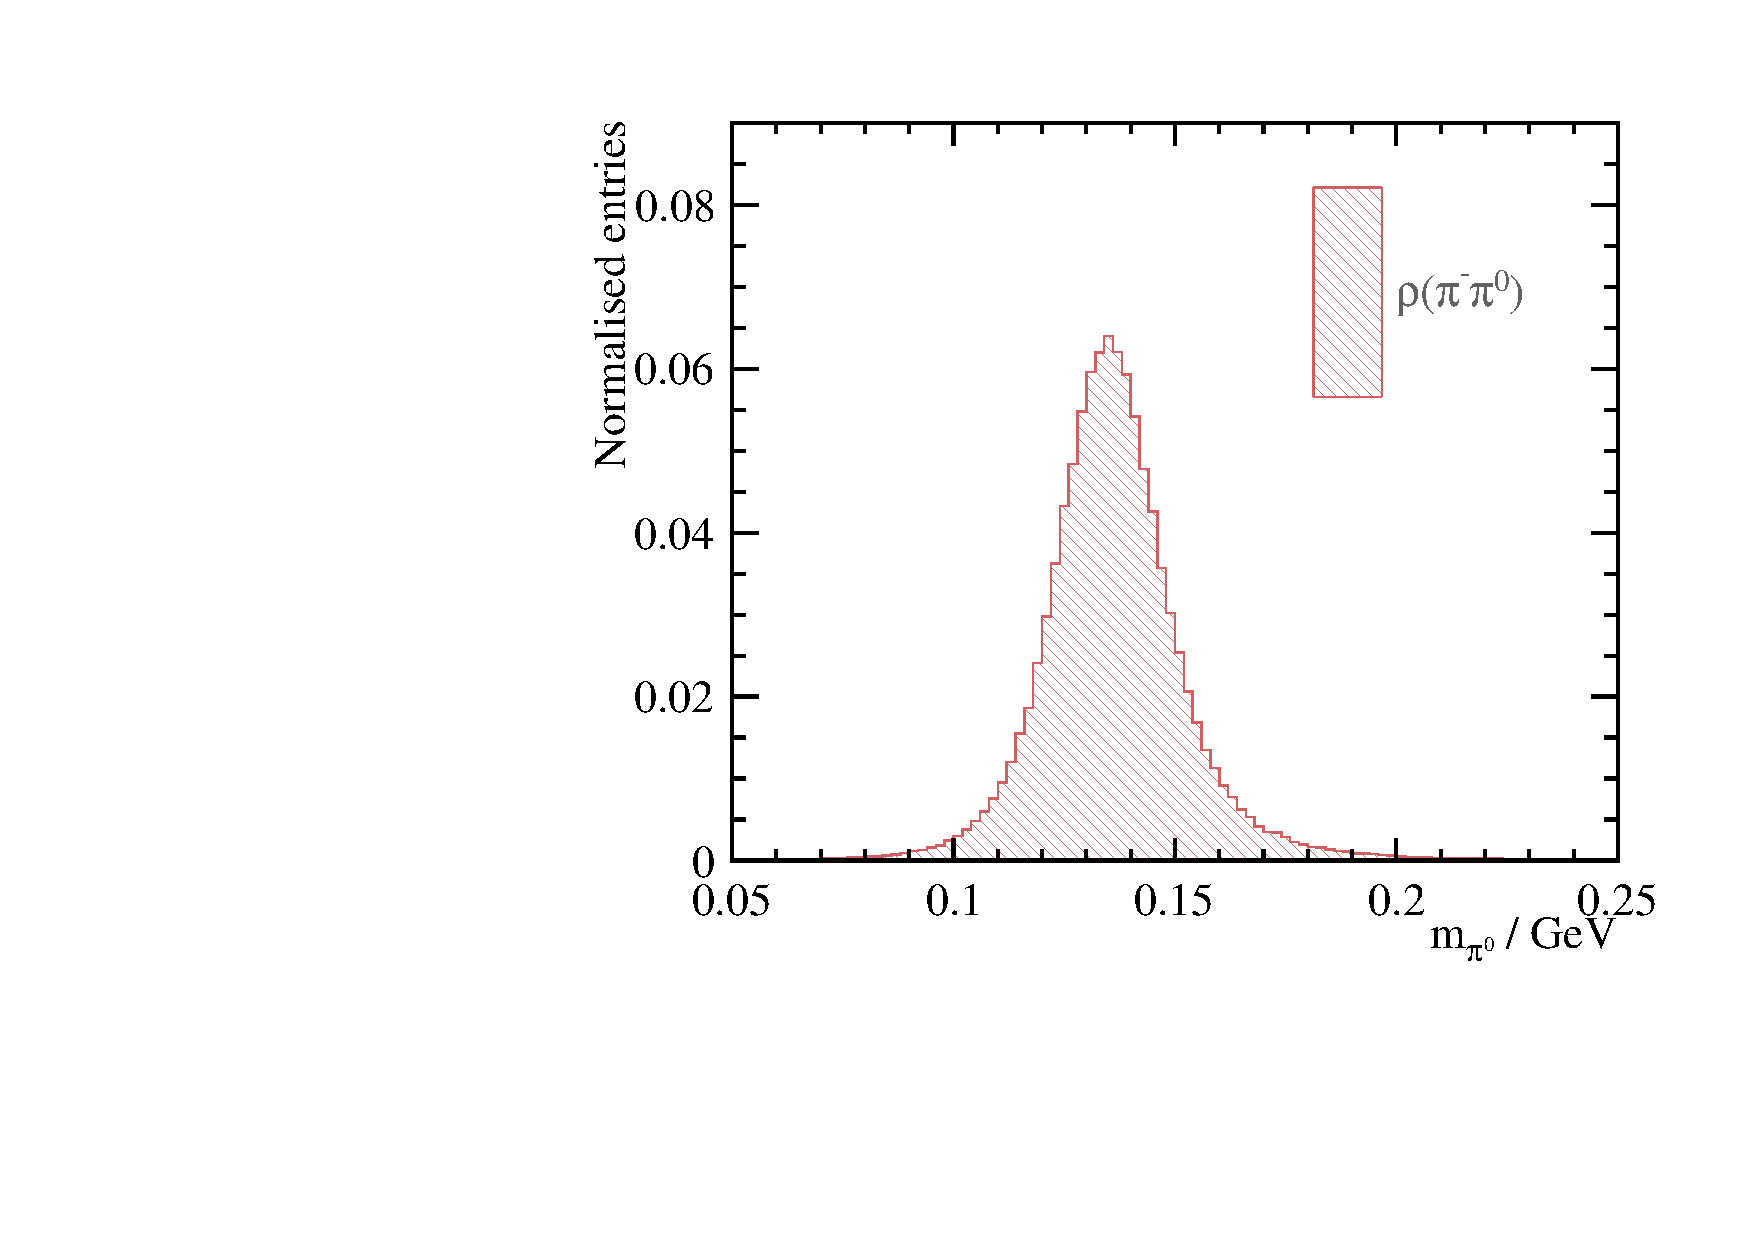
\includegraphics[width=\textwidth]{tau/mPionRhoFit_100GeV_improved_zoom.pdf}
  \caption{}
  \label{fig:tauPionFromRho}
\end{subfigure}
\begin{subfigure}[b]{0.45\textwidth}
 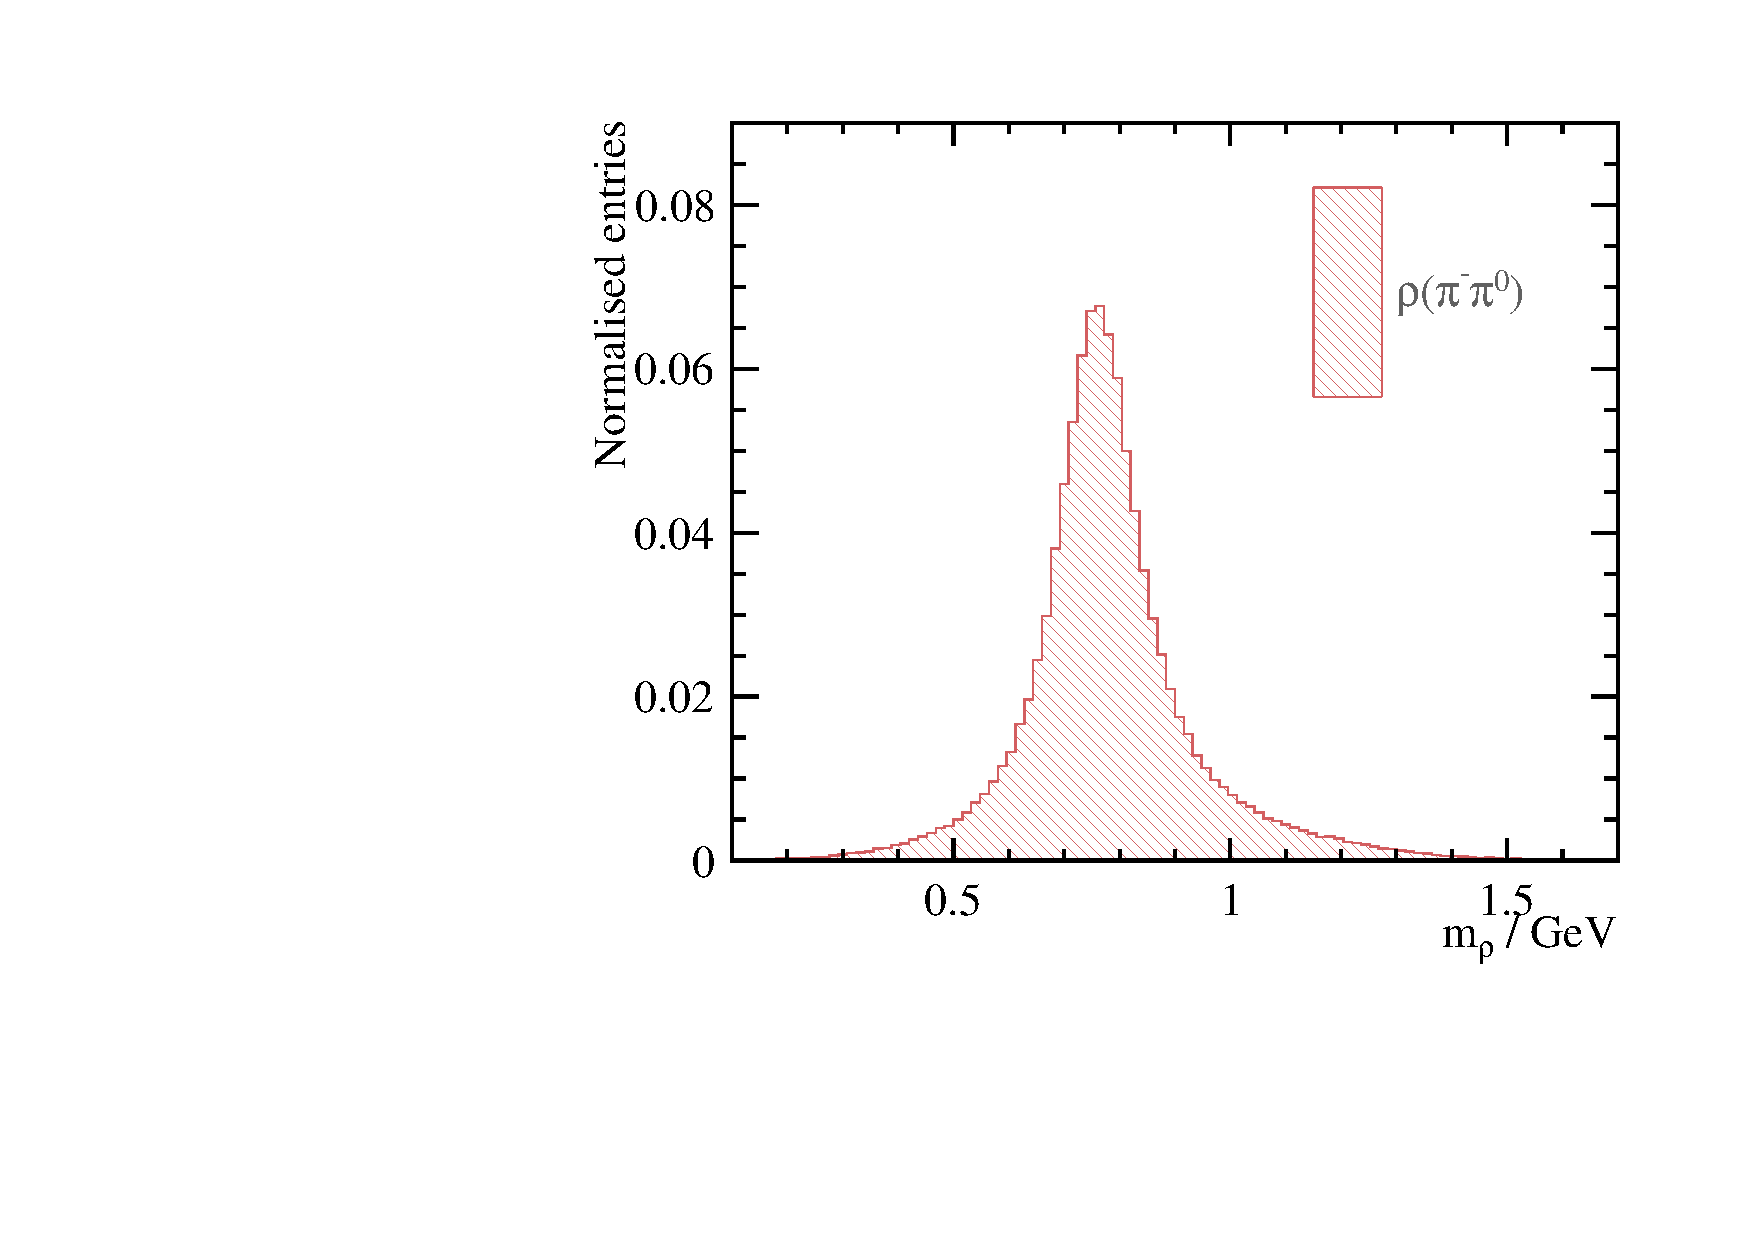
\includegraphics[width=\textwidth]{tau/mRhoRhoFit_100GeV_improved_zoom.pdf}
  \caption{}
  \label{fig:tauRhoFromRho}
\end{subfigure}
\caption
{Reconstructed invariant mass distributions for a) \Ppizero; b) \Prho, in the \decayRhoShort decay mode. The reconstructed masses are obtained using the MC truth information to find the corresponding reconstructed particles. The decay mode is selected using the MC truth information. The area under the curve is normalised to unity.}
\label{fig:tauRho}
\end{figure}



% and $\sigma_{\Ppizero}$ are assumed

%the respective half widths of the invariant mass distributions of reconstructed \Prho and \Ppizero.



%The minimisation function is iterated over all combinations of photons and \Pgpm.




%By choosing the combination of photons and \Pgpm which minimises the  $\chi^{2}$ function, the fitted \Prho mass, $m_{tot}$, and the fitted \Ppizero mass, $m_{\Pphoton_1\Pphoton_2}$, are obtained.

The $\chi^2$ function in \Equation{eqn:tauRho} is modified for the \decayAiPhotonShort decay mode hypothesis test:
%The \decayAiPhotonShort decay mode identification can be enhanced using an similar minimisation function, $\chi^2$:
\begin{equation}
\chi^{2} = {\left(\frac{m_{tot} -  m_{\Pai}}{\sigma_{\Pai}}\right)}^{2} + {\left(\frac{m_{\Pphoton_1 \Pphoton_2} -  m_{\Ppizero}}{\sigma_{\Ppizero}}\right)}^{2}  + {\left(\frac{m_{\Pphoton_3 \Pphoton_4} -  m_{\Ppizero}}{\sigma_{\Ppizero}}\right)}^{2} \,,
\label{eqn:tauA1}
\end{equation}
where the \Prho mass has been replace by the \Pai mass and other variables are defined in the same way as  previously. Four photons and one \Pgpm are required for this minimisation. To resolve the degeneracy between two photon pairs,  the requirement of $\absOf{ m_{\Pphoton_1\Pphoton_2} - m_{\Ppizero}} < \absOf{ m_{\Pphoton_3\Pphoton_4} - m_{\Ppizero}}$ is imposed.

The particle ID of charged pions and photons come from the output of the \pandora reconstruction. If there are at least four photons in an event, combinations of photons are iterated and the combination with the smallest value of $\chi^2$ is chosen. If there are two (three) photons in an event, the last term in the \Equation{eqn:tauA1}  is dropped and the $\chi^{2}$ function becomes:
\begin{equation}
\chi^{2} = {\left(\frac{m_{tot} -  m_{\Pai}}{\sigma_{\Pai}}\right)}^{2} + {\left(\frac{m_{\Pphoton_1 \Pphoton_2} -  m_{\Ppizero}}{\sigma_{\Ppizero}}\right)}^{2}  \,,
\end{equation}
where $m_{tot}$ is the invariant mass of the charged pion and two  (three) photons. If there is only one photon in an event, the $\chi^{2}$ function becomes:
\begin{equation}
\chi^{2} = {\left(\frac{m_{tot} -  m_{\Pai}}{\sigma_{\Pai}}\right)}^{2} \,,
\end{equation}
where $m_{tot}$ is the invariant mass of the charged pion and the photon.

% If there is only one photon in an event, the second term in the \Equation{eqn:tauRho} is dropped and the $\chi^{2}$ function becomes:
%\begin{equation}
%\chi^{2} = {\left(\frac{m_{tot} -  m_{\Prho}}{\sigma_{\Prho}}\right)}^{2} \,,
%\end{equation}
%where $m_{tot}$ is the total invariant mass of one photon and one \Pgpm.



 %The invariant mass of the first two photon, $m_{\Pphoton_1\Pphoton_2}$, is defined to be closer to  the invariant mass of the \Ppizero than that of the last two photon, $m_{\Pphoton_3\Pphoton_4}$. The  minimised the  $\chi^{2}$ function provides the fitted \Pai mass, $m_{tot}$, the first fitted \Ppizero mass, $m_{\Pphoton_1\Pphoton_2}$, and the second fitted \Ppizero mass, $m_{\Pphoton_3\Pphoton_4}$.

%he first photon pair is defined to have a invariant mass closer to the invariant mass of the \Ppizero than the second photon pai
% The invariant masses of photon pairs are required to be consistent with the \Ppizero mass.
%To avoid the ambiguity of the  , i
%Comparing to simple invariant mass distribution in \Figure{fig:tauVarMVis}, \decayAiPhotonShort mass peak is enhanced.
%\decayAiPhotonShort reconstruction &  \multicolumn{1}{R{0.6\textwidth}}{  $m_{\Pgpz}\parenths{\Pai}$, $m^*_{\Pgpz}\parenths{\Pai}$, $m_{\Pai}$} \\

%The  minimisation functions for \Prho and \Pai  hypothesis tests are adapted for events where the event reconstruction fails to reconstruct enough photons. Relevant terms in \Equation{eqn:tauRho} and \Equation{eqn:tauA1} are dropped if there are fewer photons reconstructed  than required in the $\chi^{2}$ functions.





Following the discussion on the \Prho invariant mass resonance reconstruction for the \decayRhoShort  decay mode,  two variables are used in the MVA classification to help to identify  \decayRhoShort  decay mode: the fitted \Prho mass ($m_\rho \equiv m_{tot}$ in \Equation{eqn:tauRho}) and the fitted \Ppizero mass ($m_{\Pgpz\parenths{\rho}} \equiv m_{\Pphoton_1\Pphoton_2}$ in  \Equation{eqn:tauRho}).

For the \decayAiPhotonShort decay mode identification using the \Pai invariant mass resonance reconstruction, three variables are used in the MVA classification:  fitted \Pai mass ($m_{\Pai} \equiv m_{tot}$ in \Equation{eqn:tauA1}), the first fitted \Ppizero mass ($m_{\Pgpz(\Pai)} \equiv m_{\Pphoton_1\Pphoton_2}$ in \Equation{eqn:tauA1}), and the second fitted \Ppizero mass ($m^*_{\Pgpz(\Pai)} \equiv  m_{\Pphoton_3\Pphoton_4}$ in \Equation{eqn:tauA1}).

 \FIGURE{fig:tauVarMA1} shows the distributions of  $m_{\Pai}$ under \decayAiPhotonShort decay mode hypothesis test for four different tau decay modes. Only the distribution for \decayAiPhotonShort decay mode has a resonance peak at \Pai mass position.

% \Equation{eqn:tauRho} and \Equation{eqn:tauA1}
%are the invariant mass of the two photons in the fit, $m_{\Pgpz}\parenths{\rho}$, and  the invariant mass of the  two photons and one \Pgpm, $m_\rho$.
%Three variables obtained in this minimisation and used in the MVA classification are the invariant mass of the first two photons in the fit, $m_{\Pgpz}\parenths{\Pai}$; the invariant mass of the last two photons in the fit, $m^*_{\Pgpz}\parenths{\Pai}$; and the invariant mass of the four photons and one \Pgpm, $m_{\Pai}$. The first photon pair is defined to have a invariant mass closer to the invariant mass of the \Ppizero than the second photon pair.

\subsection{Separating electrons from charged prions}

The particle ID output by \pandora is used extensively to reconstruct variables. However, extra variables are used in this analysis to help further separating  electrons from charged pions, obtained from a modified private version of \pandora.

%, which could be mistaken as \Pgpm in the  reconstruction.

%In particular \pandora uses a wide range of information to determine the electron ID.

An electron develops a characteristic EM shower in the \ECAL, whilst a charged pion develops a hadronic shower. Variables characterising the  EM shower helps to identify an electron. Three variables are used in the MVA classification: the start layer of the longitudinal shower ($t_0$); the fractional difference between observed and expected longitudinal shower profile describing the longitudinal EM shower ($\delta{l}$); and $\langle{w}\rangle$, a measure of the EM shower transverse width. These variables are defined in the same way as the variables used in the photon likelihood classifier in the photon reconstruction in \pandora, described in \Section{sec:photonLikelihood}.

Another type of information to differentiate an EM shower from a hadronic shower is the calorimeter hit information. Two variables used in the MVA classification are: the average energy of a calorimeter hit ($\bar{E}_{hit}$) and the average fraction of minimum ionising calorimeter hits for all particles ($\%MIP$)

Last information used to separate an electron  from a charged prion is the track$-$momentum calorimeter$-$energy consistency check. The variable used in the MVA classification is the average calorimeter energy divided by the track momentum ($\Delta E/P$).


%This variable is found to help to differentiate \decayElectronShort from \decayPionShort final state.


%EM shower profile & $\delta{l}$, $t_0$, $\langle{w}\rangle$ \\
%Calorimeter hit info. & $\bar{E}_{hit}$, $\%MIP$ \\
%Track info. & $\Delta E/P$ \\




\begin{figure}[htbp]
\centering
% \begin{center}/\end{center} takes some additional vertical space
\begin{subfigure}[b]{0.45\textwidth}
 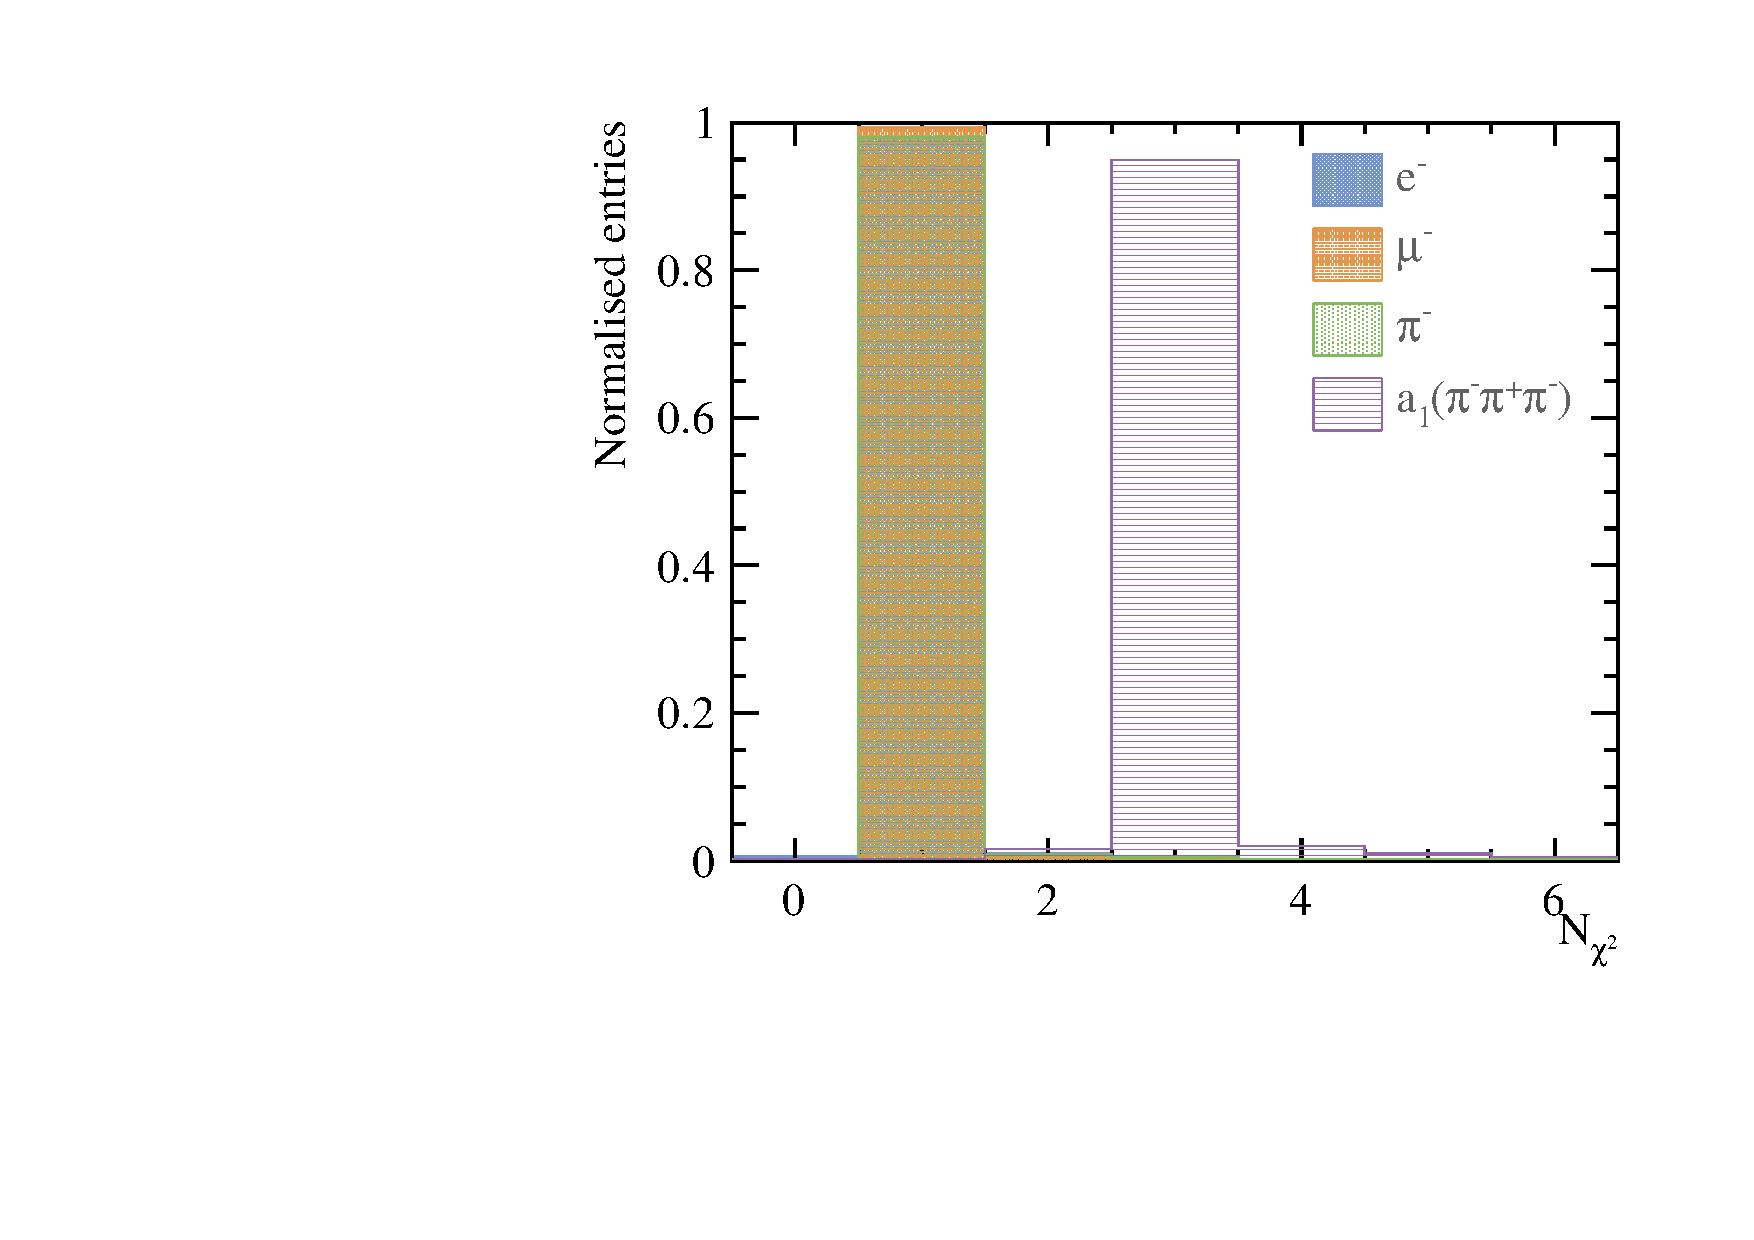
\includegraphics[width=\textwidth]{tau/var2/nCharge_100GeV_improved.pdf}
  \caption{}
  \label{fig:tauVarNCharge}
\end{subfigure}
\begin{subfigure}[b]{0.45\textwidth}
 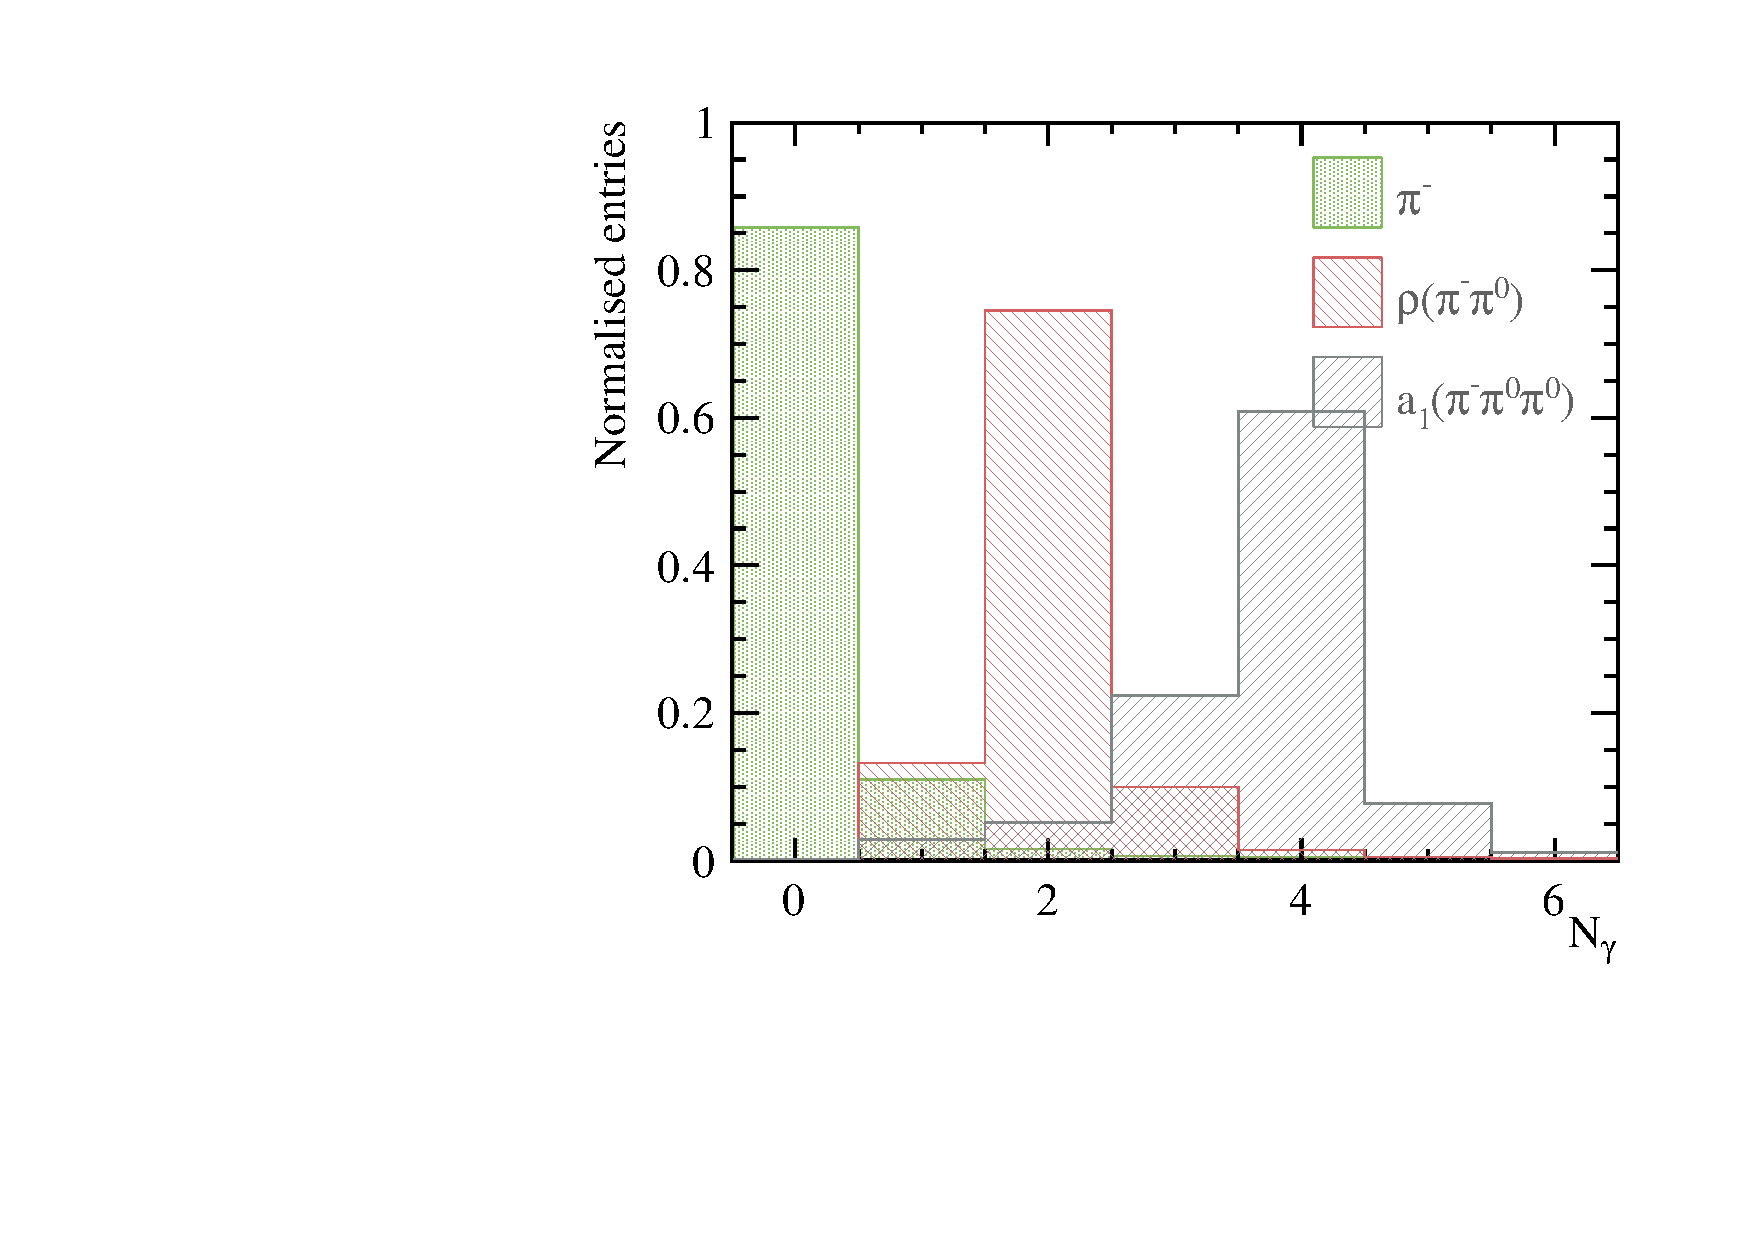
\includegraphics[width=\textwidth]{tau/var2/nPhoton_100GeV_improved.pdf}
  \caption{}
  \label{fig:tauVarNPhoton}
\end{subfigure}
\begin{subfigure}[b]{0.45\textwidth}
 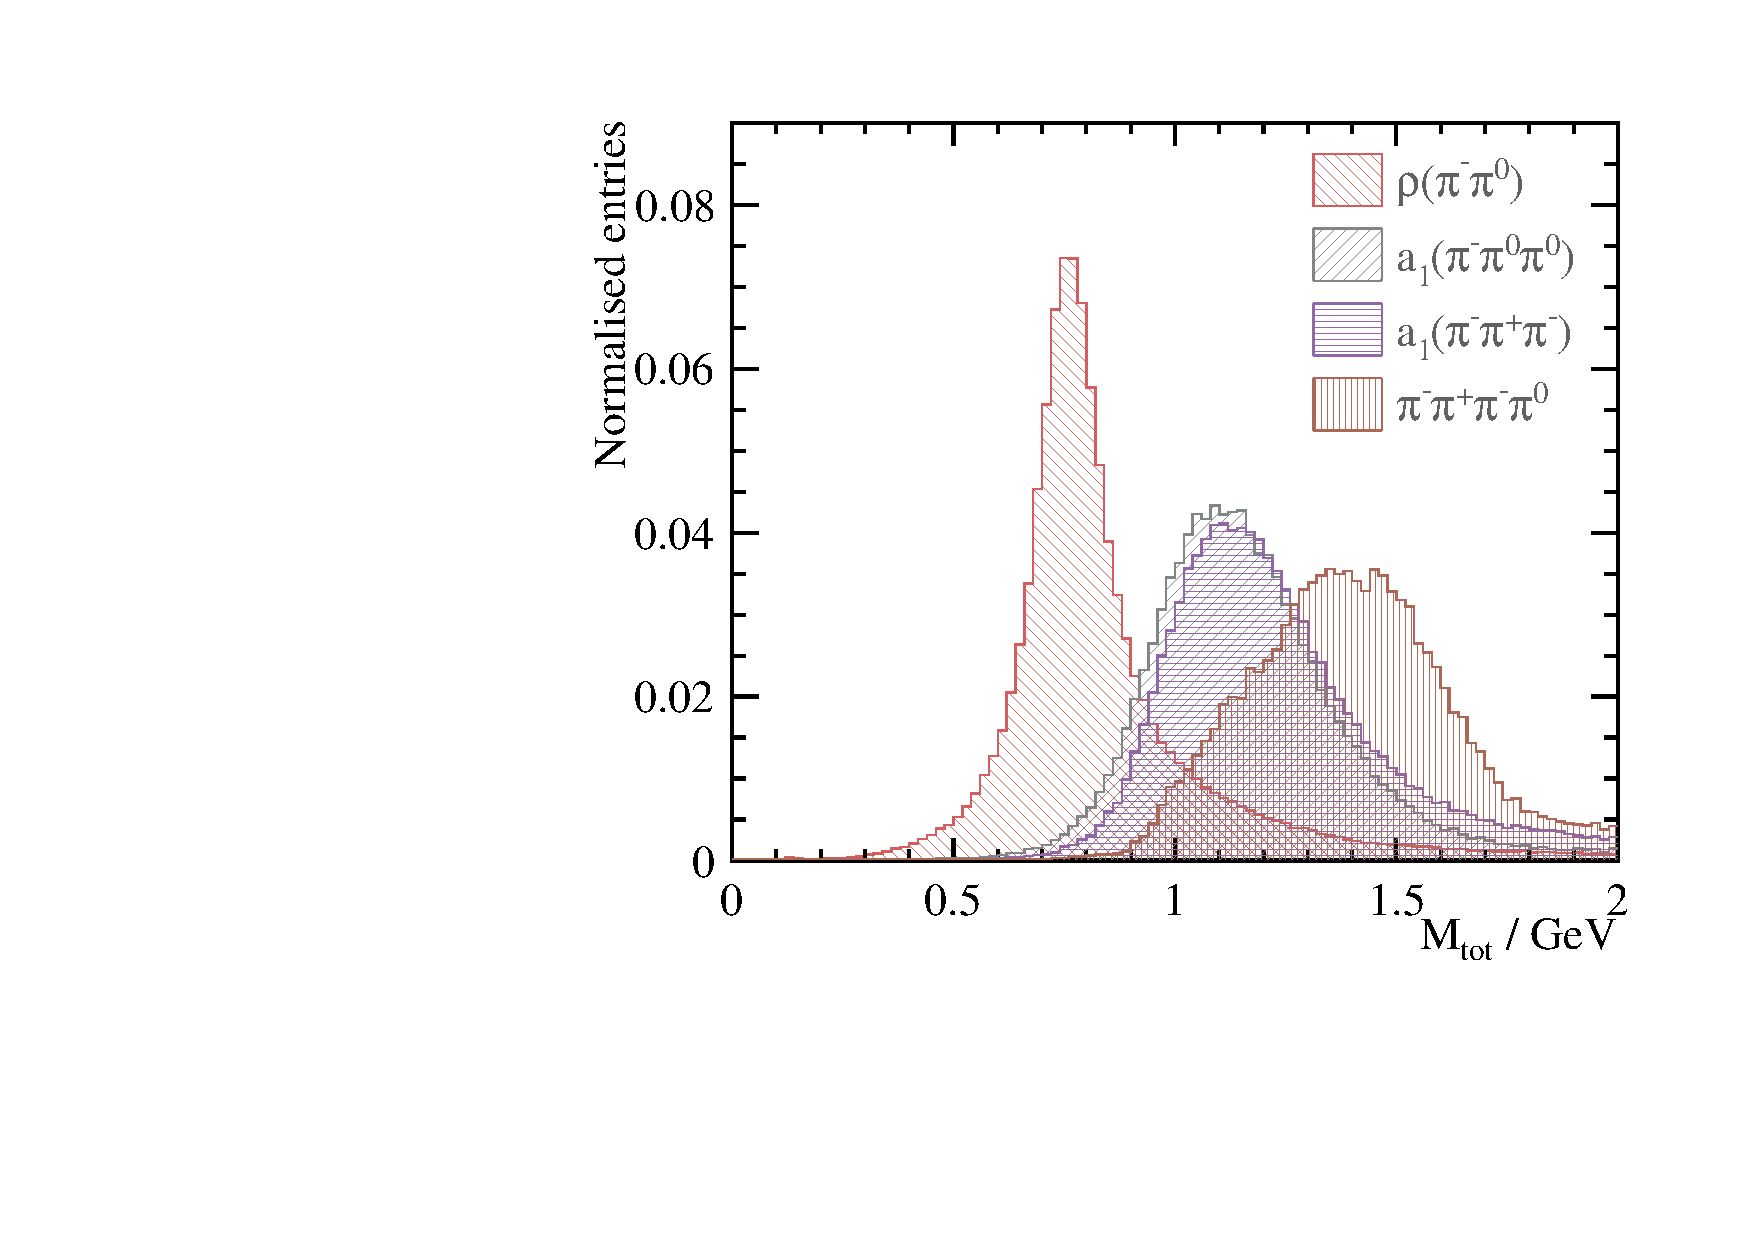
\includegraphics[width=\textwidth]{tau/var2/mVis_100GeV_improved_zoom.pdf}
  \caption{}
  \label{fig:tauVarMVis}
\end{subfigure}
\begin{subfigure}[b]{0.45\textwidth}
 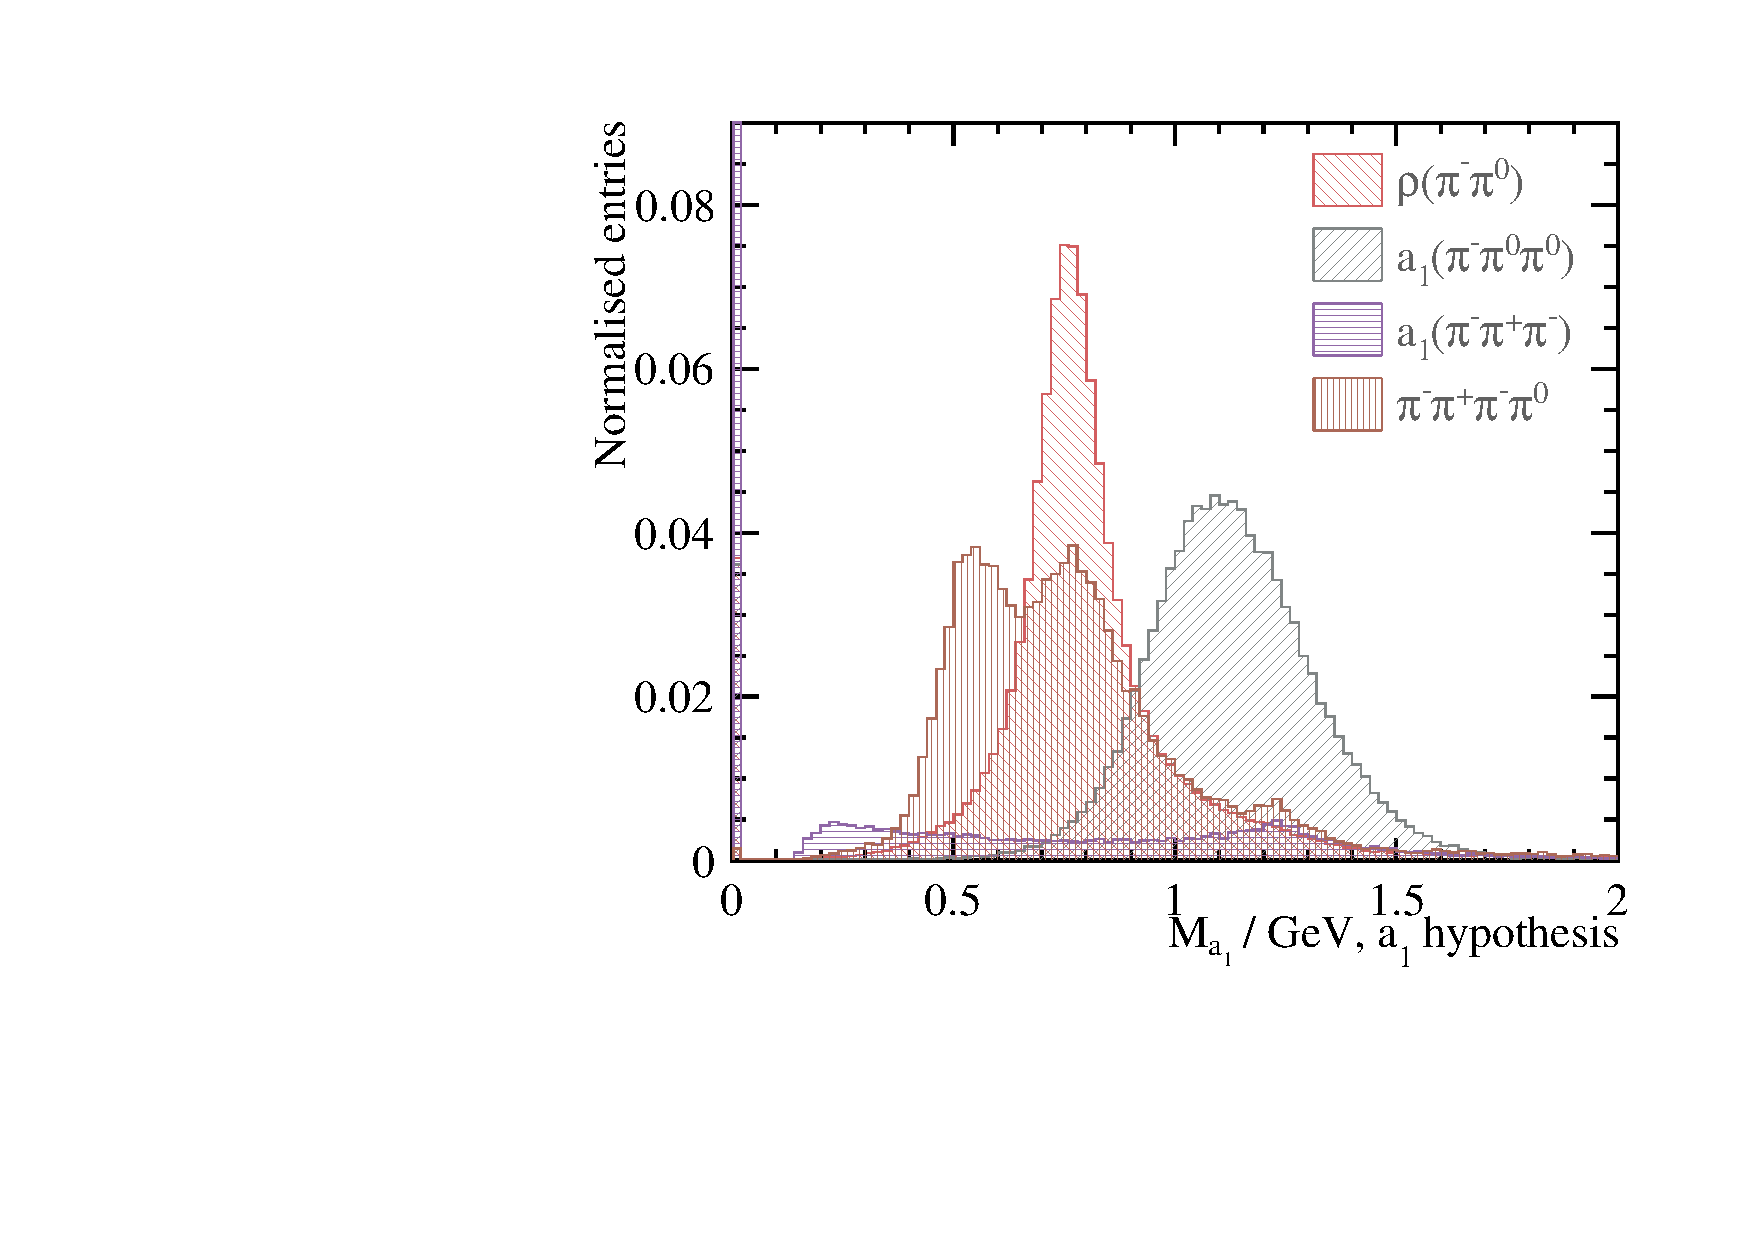
\includegraphics[width=\textwidth]{tau/var2/mA1A1Fit_100GeV_improved_zoom.pdf}
  \caption{}
  \label{fig:tauVarMA1}
\end{subfigure}

\caption
{Distributions for a) the number of charged particle (${N}_{\charge}$); b) the number of photons (${N}_{\Pgg}$); c) the invariant mass of all non-neutrino decay products ($m_{vis}$); and d) the fitted invariant mass of the \Pai ($m_{\Pai}$), reconstructed with \decayAiPhotonShort decay mode hypothesis. Area under the curve for each decay mode is normalised to 1. Decay modes in all plots are selected using the truth information.}
\label{fig:tauVar}
\end{figure}


\section{Multivariate Analysis}
\label{sec:tauMVA}

For the multivariate analysis, the \multiclass class of the TMVA package \cite{Therhaag:2009dp} was used to perform a multiple-class classification, which classifies seven tau lepton decay final states simultaneously. The \multiclass classification is an extension of a standard two-class signal$-$background classification. The classifier used  is Boosted Decision Tree classifier with Gradient boost (BDTG). Half of the randomly selected samples were used in the training process and the other half were used for testing. The optimisation of the BDTG classifier followed the strategy outlined in \Section{sec:pandoraMVAoptimisation}. The optimised parameters for the classifier are listed in \Table{tab:tauBDTparameters}, where an explanation of the parameters can be found in \Section{sec:pandoraMVAbdtVar}.

% The discussion on multivariate analysis can be found in \Section{sec:pandoraMVA}. In particular, the \multiclass classifier is discussed in \Section{sec:pandoraMVAmulticlass}.



\begin{table}[!htbp]\centering
%\small
\begin{tabular}{lr}
\hline \hline
 Parameter &  Value \\
\hline
Depth of tree & 5 \\
Number of trees & 3000 \\
Boosting & gradient boost \\
Learning rate of the gradient boost & 0.1 \\
Metric for the optimal cuts & Gini Index \\
Bagging fraction & 0.5 \\
Number of bins per variables & 100 \\
End node output & yes/no \\
\hline \hline
\end{tabular}

\caption
{Optimised parameters for the Boosted Decision Tree with Gradient boost \multiclass classifier. A detailed explanation of variables can be found in \Section{sec:pandoraMVAbdtVar}.}
\label{tab:tauBDTparameters}
\end{table}


\section{Tau decay mode classification efficiency}
\label{sec:tauClassificationEff}
The classification efficiencies for the seven tau decay modes are shown in \Table{tab:TauSelExample}. The correct classification efficiencies are shown in bold numbers in the table, defined as:
\begin{equation}
\varepsilon_i = \frac{N^{correct}_i}{N^{MC}_i},
\label{eqn:tauEff}
\end{equation}
where $N^{correct}_i$ is the number of correctly classified events for tau decay mode $i$ and the $N^{MC}_i$ is the number of events for tau decay mode $i$, based on the truth information.
%For example, 99.8\% events of true \decayElectronShort decay mode are reconstructed correctly.

For the \decayElectronShort decay mode,   99.8\%  correct classicisation efficiency is achieved. For the \decayMuonShort decay mode,  99.5\% correct classicisation efficiency is achieved.

% due to an effective track reconstruction and muon reconstruction algorithms in \pandora.

For the \decayPionShort decay mode, 3.4\% events are misclassified as \decayRhoShortest decay mode events. If the reconstruction is unable to reconstruct two photons from \Ppizero decay in \decayRhoShortest decay mode, the \decayPionShort and \decayRhoShortest decay modes events would appear to be similar and misclassification occurs. On the other hand, only 0.9\% of \decayPionShort decay events are misclassified as \decayElectronShort decay, due to variables dedicated to separation between \Pem and \Ppiminus.

%The confusion with \decayElectronShort is at percent level, which is low due to the usage of EM shower variables. The percent level confusion with \decayAiPionShortest is because the tracking efficiency is at 98\%, where 2\% \decayPionShort events have more than one track reconstructed.

%confusion with \decayRhoShortest decay mode  is to due to differentiate two event topologies. Around 15\% of \decayPionShort events have at least one photon reconstructed, mostly due to the FSR.

For the \decayRhoShortest decay mode, most misclassification comes from the confusion with \decayAiPhotonShortest decay mode.  If the reconstruction is unable to resolve the all photons from \Ppizero decay in \decayRhoShortest and \decayAiPhotonShortest decay mode, the two decay modes would have similar topologies.

For the \decayAiPhotonShortest decay mode, the correct classification rate is the lowest among seven decay modes, as the final state of the \decayAiPhotonShortest decay mode is the most challenging to reconstruct correctly with four photons in the final state. The 9.5\% confusion with \decayRhoShortest decay mode is due to the same photon reconstruction failure issue. It should be noted that the distribution of the number of photons in \Figure{fig:tauVarNPhoton} suggests that 30\% of \decayAiPhotonShortest events have fewer than four photons reconstructed, overlapping with the distribution for \decayRhoShortest decay mode. The \decayAiPhotonShortest resonance reconstruction and the use of the MVA \multiclass classifier reduce the confusion between two decay modes from 30\% to  9.5\%.

%For the \decayAiPionShortest decay mode, the biggest source of misclassification is with \decayThreePionPhotonShort decay mode. The biggest misclassification of  \decayThreePionPhotonShort decay mode  is with \decayAiPionShortest decay mode.

%And the reason is the same for

%The unprecedented high classification rate has been achieved. The improvement of photon reconstruction described in \Section{} improved the ability to separate 1-prong final state. Most notably,  \Figure{} shows number of photons have a high correct reconstruction efficiency.


\begin{table}[htbp]
\centering
\small
\smallskip
\begin{tabular}{ l   r  r  r  r  r  r  r }
\hline
\hline
Reco$\downarrow$ Truth$\to$& \decayElectronShort & \decayMuonShort &\decayPionShort & \decayRhoShortest &\decayAiPhotonShortest &\decayAiPionShortest &\decayThreePionPhotonShort \\
\hline

{\decayElectronShort}&\textbf{99.7}\%&-&0.9\%&0.6\%&0.4\%&-&-\\
{\decayMuonShort}&-&\textbf{99.5}\%&0.6\%&-&-&-&-\\
{\decayPionShort}&-&0.3\%&\textbf{94.0}\%&0.8\%&-&0.4\%&-\\
{\decayRhoShort}&-&-&3.4\%&\textbf{93.6}\%&9.5\%&0.6\%&2.3\%\\
{\decayAiPhotonShort}&-&-&-&4.5\%&\textbf{89.7}\%&-&0.6\%\\
{\decayAiPionShort}&-&-&0.9\%&-&-&\textbf{96.8}\%&6.4\%\\
{\decayThreePionPhotonShort}&-&-&-&0.3\%&-&2.0\%&\textbf{90.6}\%\\

\hline
\hline
\end{tabular}

\caption[Classification efficiency for tau decay modes.]
{ Classification efficiency for seven tau decay modes using the nominal \ILD detector model, with \eeTauTau channel at \rootSGeV{100}. Bold numbers show the correct classification efficiencies. \Pgngt is not shown. - represents a number below 0.25\%.  Statistical uncertainties are less than 0.25\%.}
\label{tab:TauSelExample}
\end{table}




\section{Electromagnetic calorimeter optimisation}
\label{sec:tauECAL}

The tau decay mode classification is used to study the \ECAL performance as a function of the \ECAL square cell sizes and the centre-of-mass energies of the \eeToTauTau events. The tau decay mode classification was repeated with varying \ECAL square cell sizes at 3, 5, 7, 10, 15 and 20\,mm, and at four  centre-of-mass energies of 100, 200, 500, 1000\,GeV. Other \ECAL dimensions are kept the same as the \ILD nominal detector. The multivariate classifier was trained  individually for each \ECAL cell size and each centre-of-mass energy.


%The analysis is repeated with varying \ECAL square cell sizes at 3, 5, 7, 10, 15 and 20\,mm, at four  \sqrtS = 100, 200, 500, 1000\,GeV.
%In above sections, an analysis on tau decay mode classification is presented. Events used in the analysis were \eeToTauTau events at \rootSGeV{100} with the nominal \ILD detector model. In this section, the analysis

As \pandora is optimised for the nominal \ILD detector, a re-optimisation is required when the study uses the detector model with non-nominal \ECAL square cell sizes. In particular, the optimal parameters used in \PhotonFragmentRemoval algorithm  have a large dependence on the \ECAL cell sizes. The optimal \ClosestHitDistance parameter in \PhotonFragmentRemoval algorithm, which is a distance metric controlling the merging of the fragment, was chosen by selecting the value that gives the highest overall classification rate (\tauHad defined in \Equation{eq:had}). \TABLE{tab:TauPhotonFragmentRemovalParameter} shows the optimised values of \ClosestHitDistance parameter in  \PhotonFragmentRemoval algorithm as a function of the \ECAL square cell size. As cell sizes become larger, the distance metric for merging photons becomes larger, as expected.

%For example, the \PhotonFragmentRemoval algorithm which merges photon fragments uses a distance metric that depends on the \ECAL cell sizes.

\begin{table}[htbp]
\centering
%\small
%\smallskip
\begin{tabular}{ l   r  r  r  r  r  r  }
\hline
\hline
\ECAL square cell size & 3\,mm & 5\,mm & 7\,mm & 10\,mm & 15\,mm & 20\,mm  \\
\hline
\ClosestHitDistance & 5\,mm & 10\,mm & 10\,mm & 10\,mm & 20\,mm & 20\,mm \\
\hline
\hline
\end{tabular}

\caption
{Optimised values of \ClosestHitDistance parameter in \PhotonFragmentRemoval algorithm as a function of the \ECAL square cell size.}
\label{tab:TauPhotonFragmentRemovalParameter}
\end{table}


Because the electron and muon reconstruction mostly rely on the performance of the tracking system, which was not varied in this study, only the   tau hadronic decay modes were investigated for the \ECAL optimisation study. The correct classification efficiencies for  tau hadronic decay final states  as a function of the \ECAL square cell sizes for different centre-of-mass energies are shown in \Figure{fig:TauPionEfficiency}. The tau decay mode correct classification efficiencies generally decrease with an increase of centre-of-mass energies and an increase of \ECAL cell sizes.

%\FIGURE{fig:TauPionEfficiency} shows that

%This trend is observed for almost all tau decay modes.

As the centre-of-mass energy increases, tau decay products are often boosted. It is increasingly difficult to separate tau decay products, for example, the photon pair from \Ppizero decay. Therefore, the inability to separate photon pairs leads to a degradation of  the classification performance.
% becomes very challenging to separate at a high centre-of-mass energy.

The change in the \ECAL cell size will change the transverse spatial resolution. Hence a large cell size will result in a low transverse spatial resolution, leading to the inability to separate a pair of photons. Consequently, a worse classification performance is expected for a large \ECAL cell size.
%An increase of the \ECAL cell sizes   degrading the classicisation performance.



%For the \decayPionShort decay mode, the general trend is followed. The efficiency for \rootSGeV{200} is slightly better than that of the \rootSGeV{100} for small cell sizes.

For the \decayRhoShort decay mode, the efficiency for  \rootSGeV{1000} increases as the cell size increases. This is because the multivariate classifier optimises for the overall classification efficiency, which may balance the decrease of the efficiency of one decay mode by the increase of the efficiency of another decay mode. In this case, the small increase in the efficiency for \decayRhoShort decay mode at \rootSGeV{1000} is compensated by the drastic decrease in the efficiency for \decayAiPhotonShort decay mode at the same centre-of-mass energy.

For the \decayAiPhotonShort decay mode, the loss of efficiency with an increasing \ECAL  cell size and an increasing centre-of-mass energy is most significant comparing to other decay modes. With most number of photons in the final state, it is the most challenging decay channel to reconstruct and thus most sensitive to the change in cell sizes and centre-of-mass energies.

For the \decayAiPionShort decay mode, the efficiencies are similar to that of the \decayPionShort decay mode. Both final states contain charged particles only. Therefore it is most sensitive to the tracking performance, which is not affected by the  varying of the \ECAL cell sizes.

%For the \decayThreePionPhotonShort decay mode, the decreases in efficiencies are more significant for \rootSGeV{500} and 1000\,GeV.

%The   correct reconstruction efficiency of the tau leptonic decay is not used as a metric as they are similar across different \ECAL cell sizes. This is because the \Pepm and \Pgmpm identifications mostly rely on the tracking system, which was not varied in this study. However the energy deposited in the calorimeter are also used for the association to the tracks. But the calorimeters have a small impact on the electron and  muon identification.

%This classification can be applied for different  \sqrtS and with different detector models. The main reconstruction issue is to separate boosted photon pair from \Ppizero decay. High \sqrtS The \ECAL cell size is crucial in separating the EM showers from photons. As discussed in previous chapter, separating photons requires a high transverse spatial resolution. Therefore, the \ECAL square cell size is expected to affect the classification efficiency.

%The main difficulty in the classification is to classify 1-prong final states.  These final states involves \Ppizero, where two photons from \Ppizero decay could be poorly reconstructed. At high energy, \Ppizero is boosted making the reconstruction more challenging. The ability to reconstruct the two photons as separate entities requires good pattern recognition algorithm for photons and \ECAL spatial resolution. Hence the improved photon reconstruction in \Chapter{chap:Photon} is used in this study. The impact of the \ECAL transverse spatial resolution on the tau decay classification is demonstrated as well.





%\FIGURE{fig:TauPionEfficiency} shows the correct classification efficiencies for  tau hadronic decay final states  as a function of the \ECAL square cell sizes. For example, plotted values for 5\,mm cell size at \rootSGeV{100} are the same as the bold numbers in \Table{tab:TauSelExample}.




\begin{figure}[htbp]
\centering % \begin{center}/\end{center} takes some additional vertical space
\begin{subfigure}[b]{0.45\textwidth}
  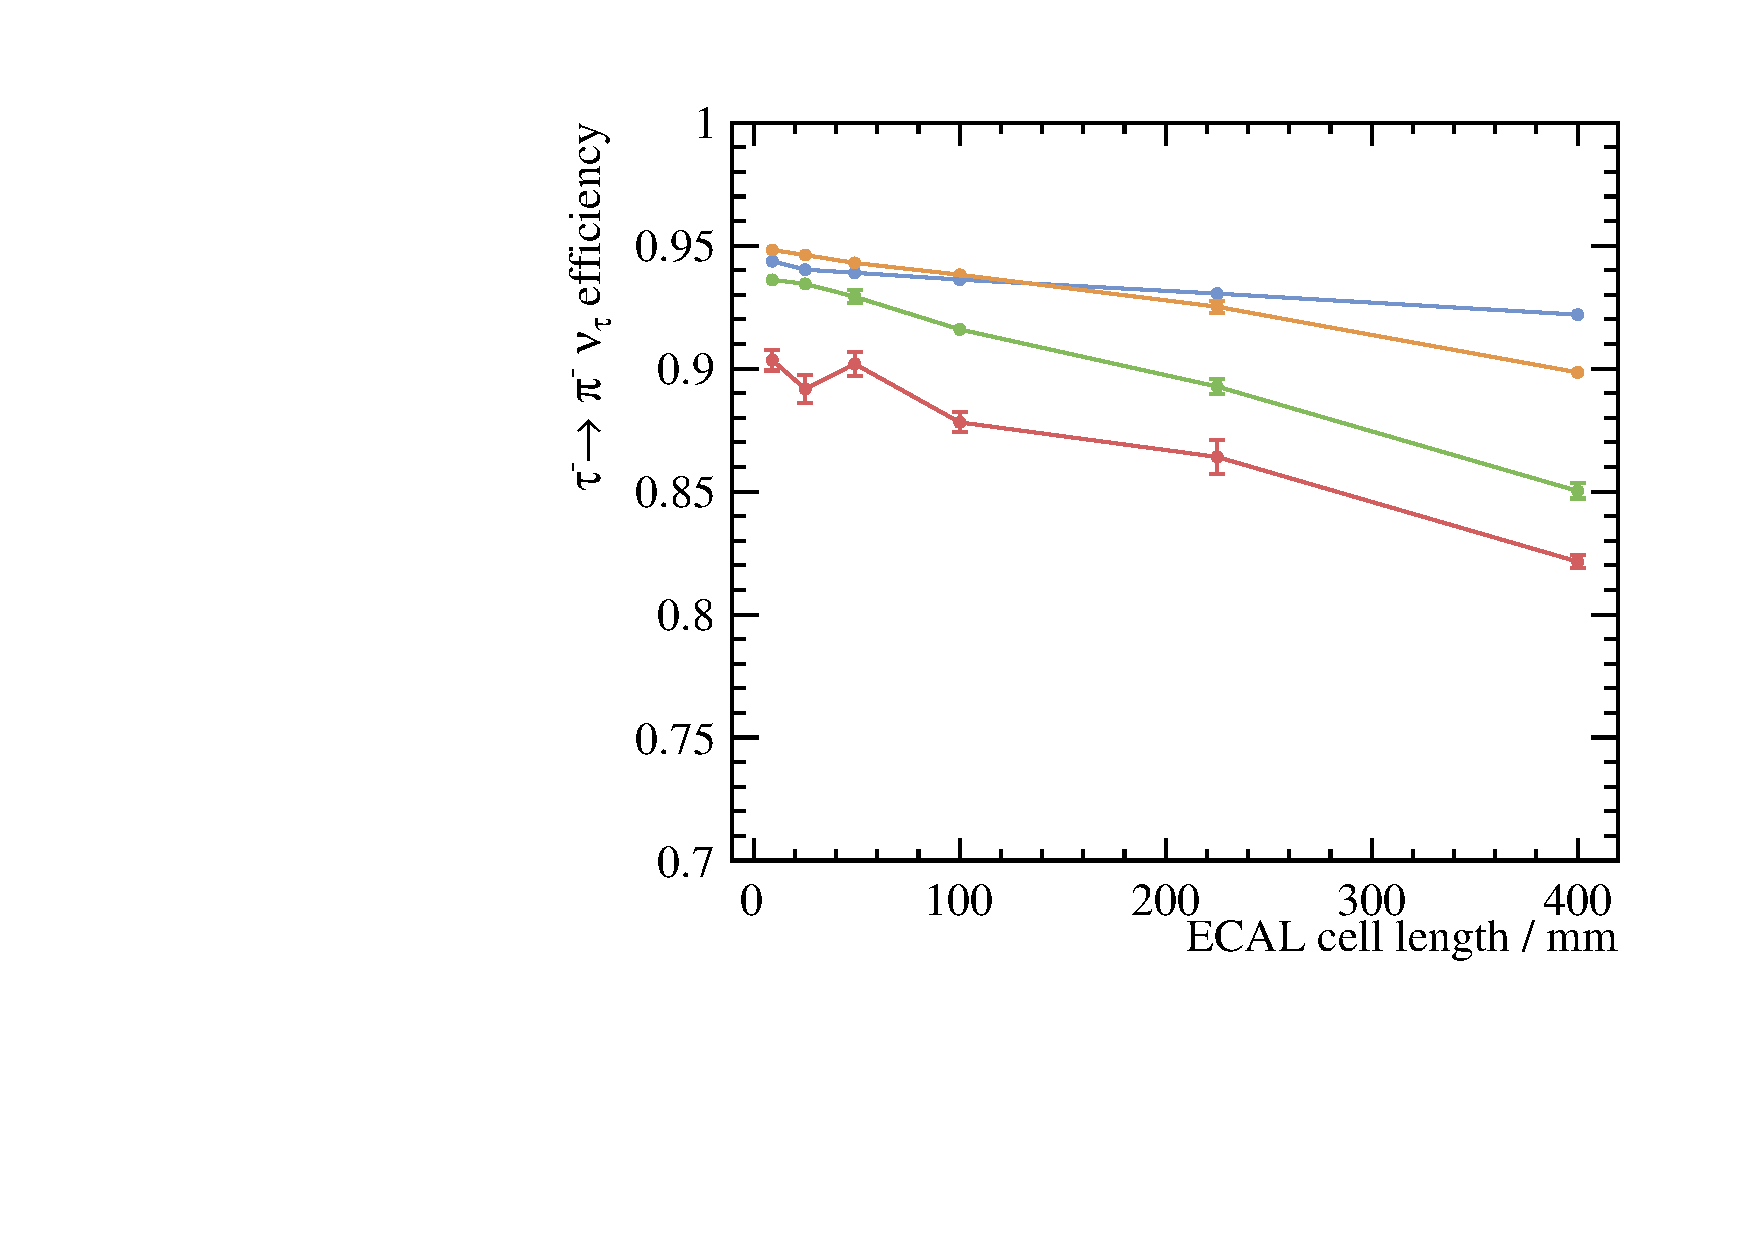
\includegraphics[width=\textwidth]{tau/plots3/decayMode2.pdf}
  \caption{}
  \label{fig:tauDecayMode2}
\end{subfigure}
\begin{subfigure}[b]{0.45\textwidth}
  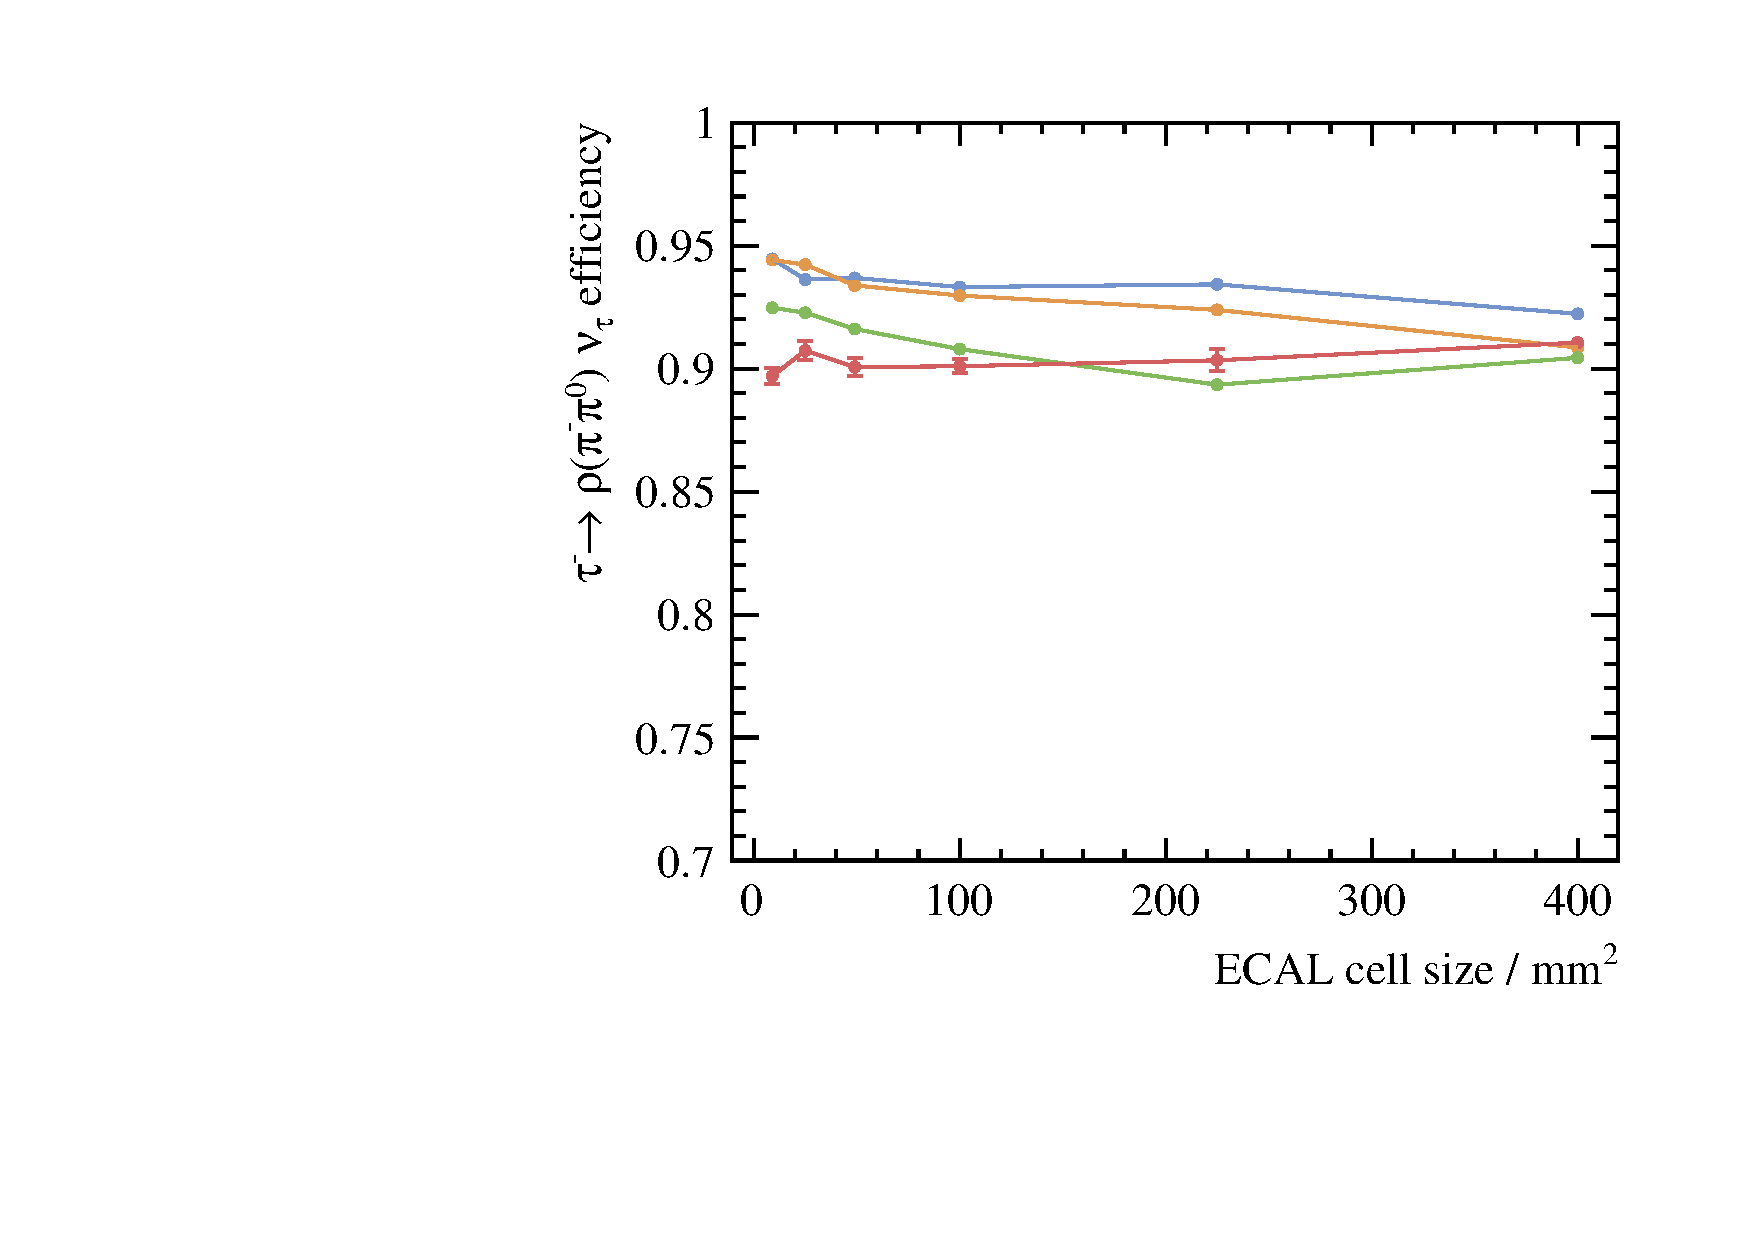
\includegraphics[width=\textwidth]{tau/plots3/decayMode3.pdf}
  \caption{}
  \label{fig:tauDecayMode3}
\end{subfigure}
\begin{subfigure}[b]{0.45\textwidth}
  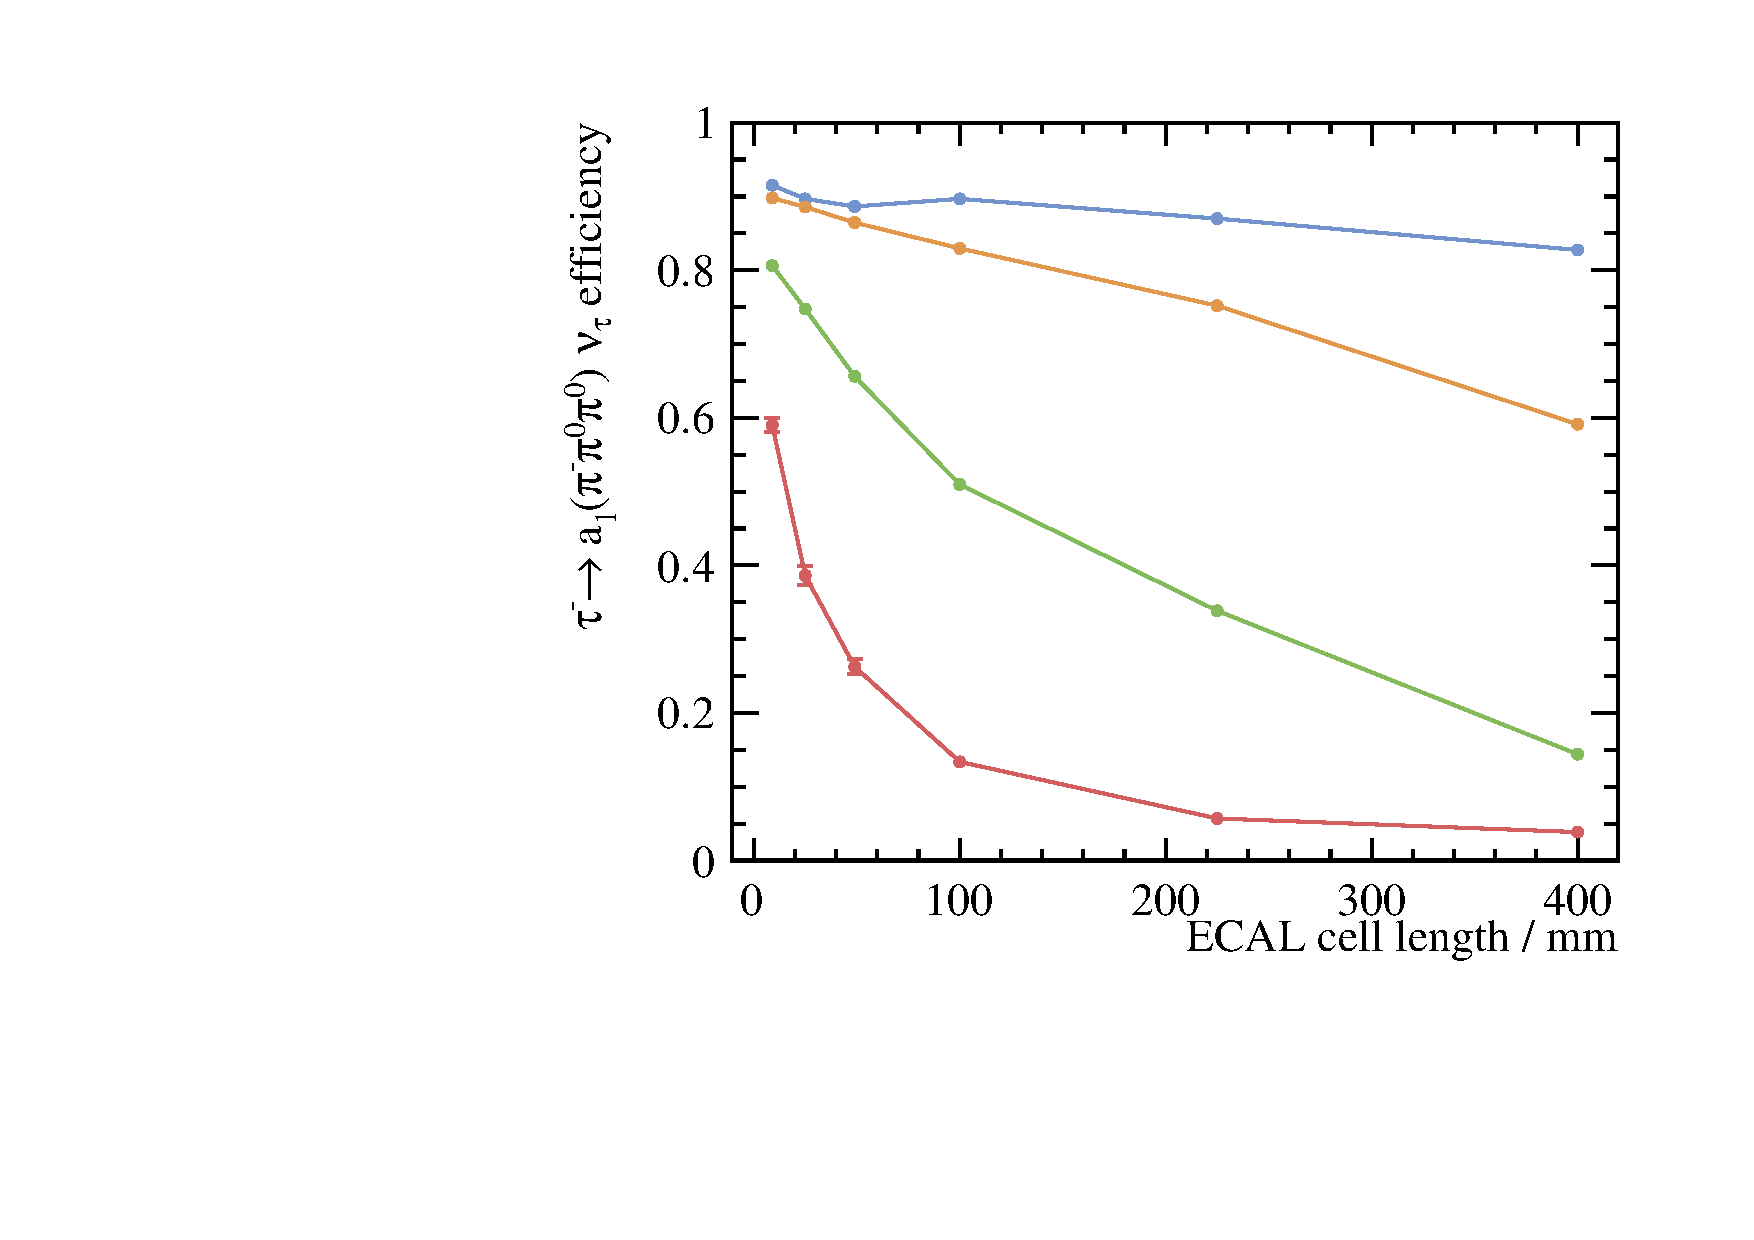
\includegraphics[width=\textwidth]{tau/plots3/decayMode4.pdf}
  \caption{}
  \label{fig:tauDecayMode4}
\end{subfigure}
\begin{subfigure}[b]{0.45\textwidth}
  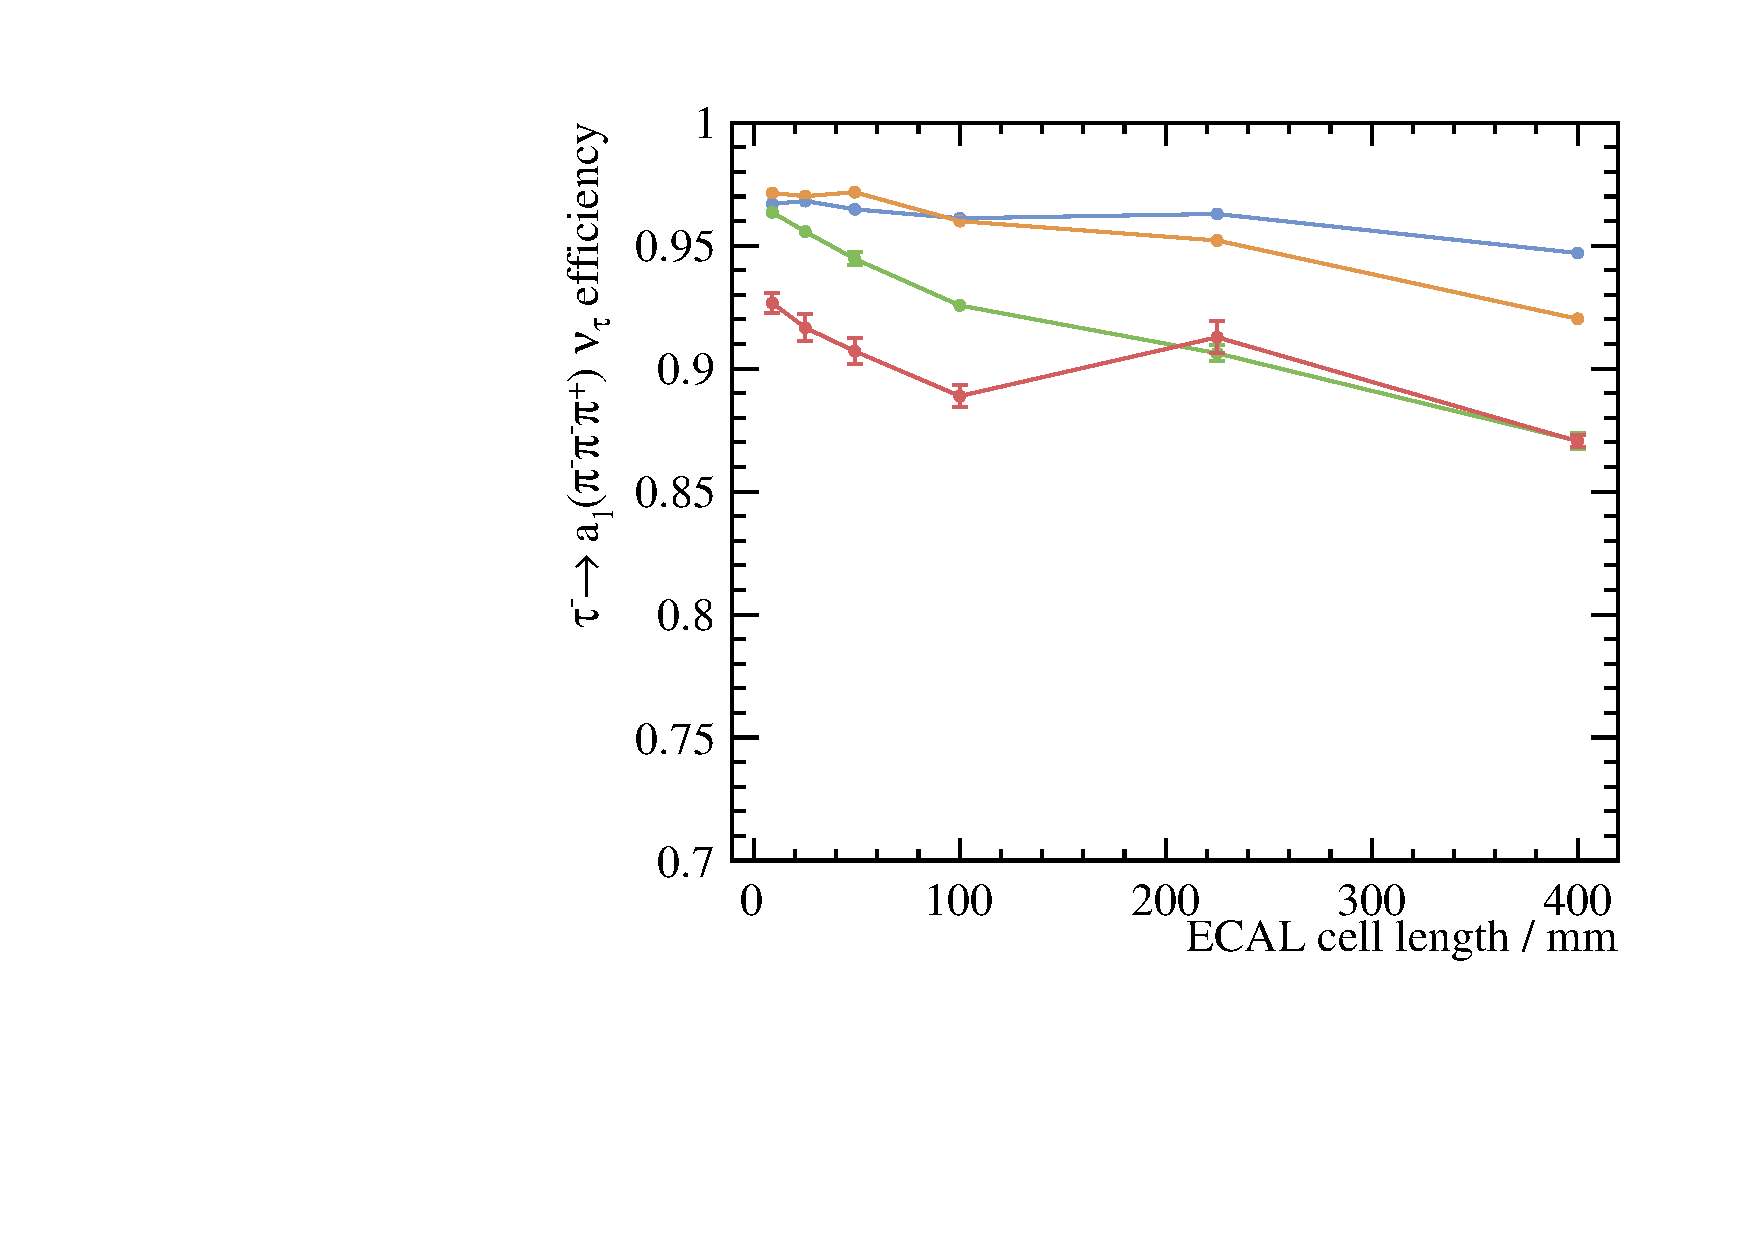
\includegraphics[width=\textwidth]{tau/plots3/decayMode5.pdf}
  \caption{}
  \label{fig:tauDecayMode5}
\end{subfigure}
\begin{subfigure}[b]{0.45\textwidth}
  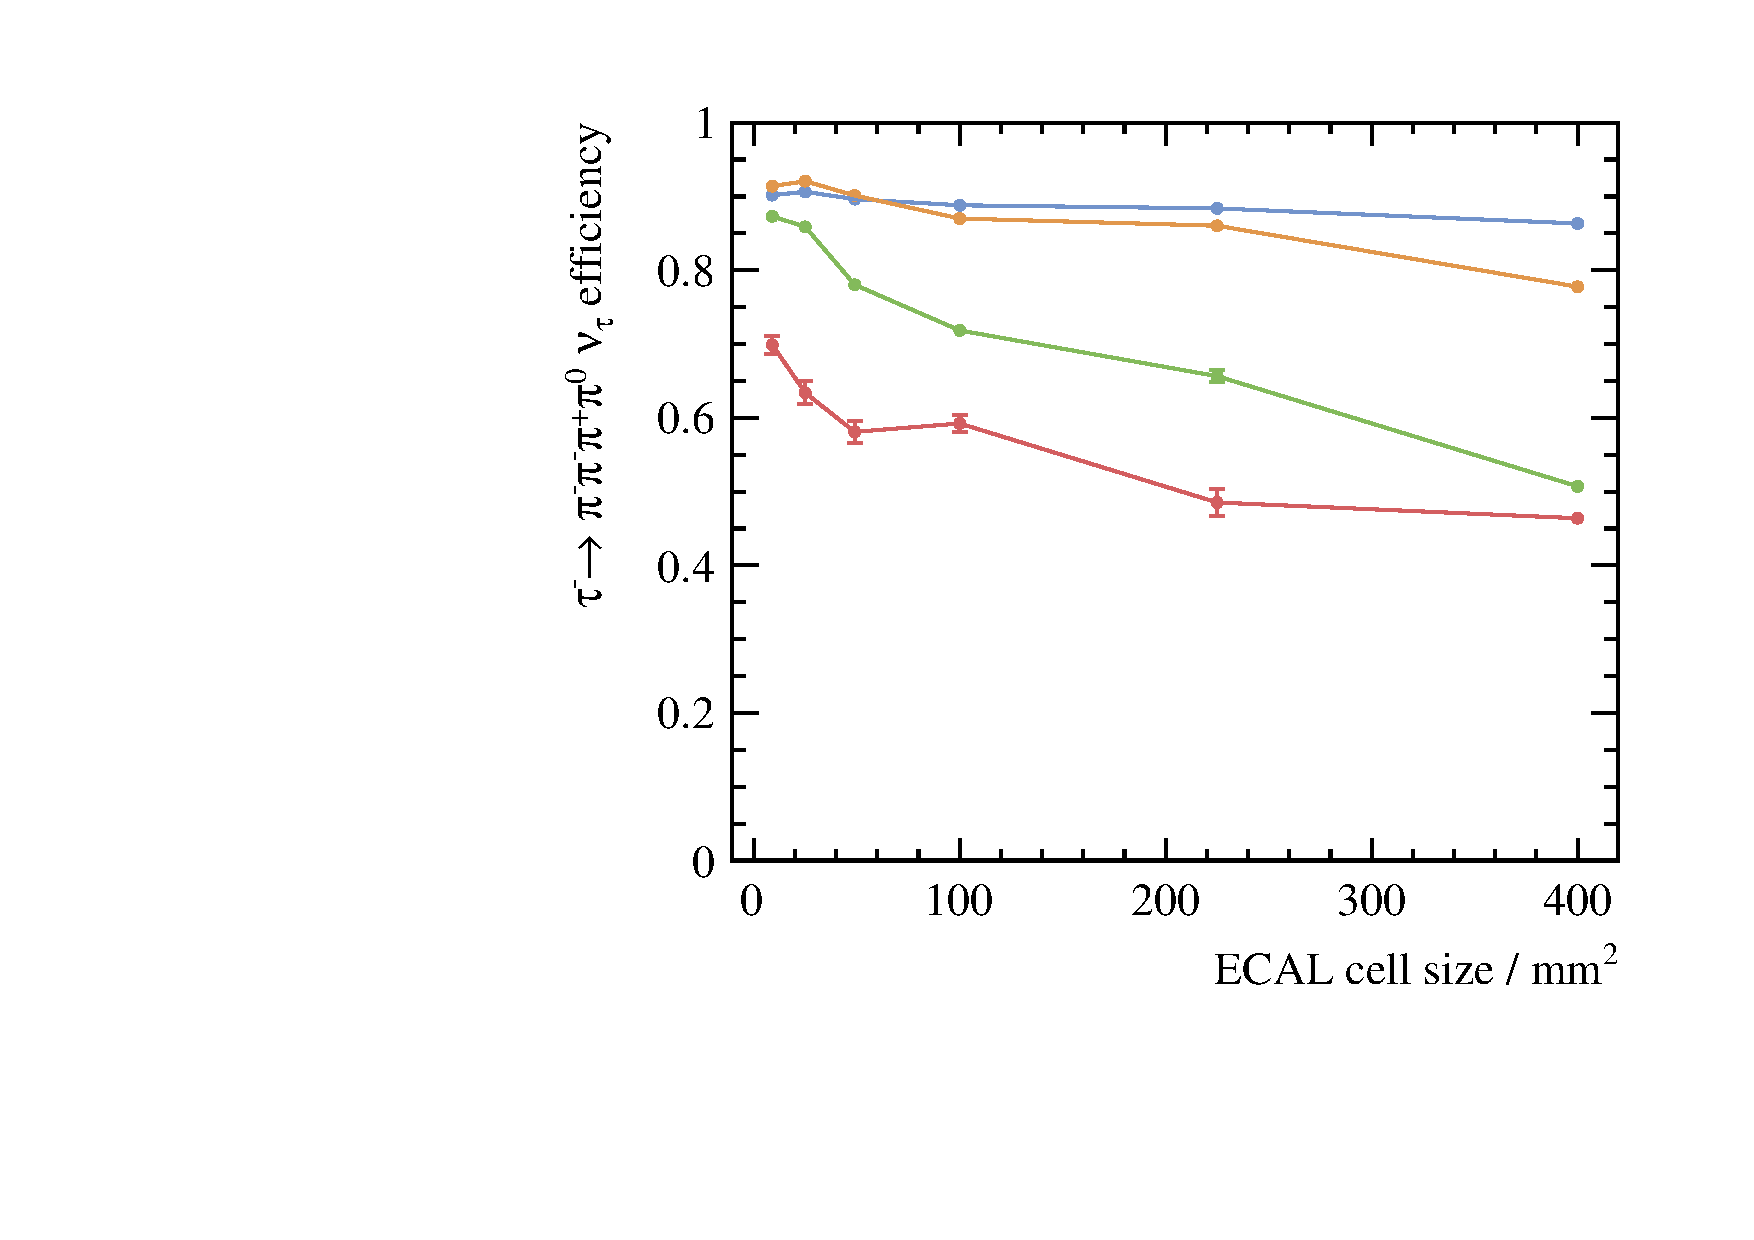
\includegraphics[width=\textwidth]{tau/plots3/decayMode6.pdf}
  \caption{}
  \label{fig:tauDecayMode6}
\end{subfigure}
\begin{subfigure}[b]{0.45\textwidth}
  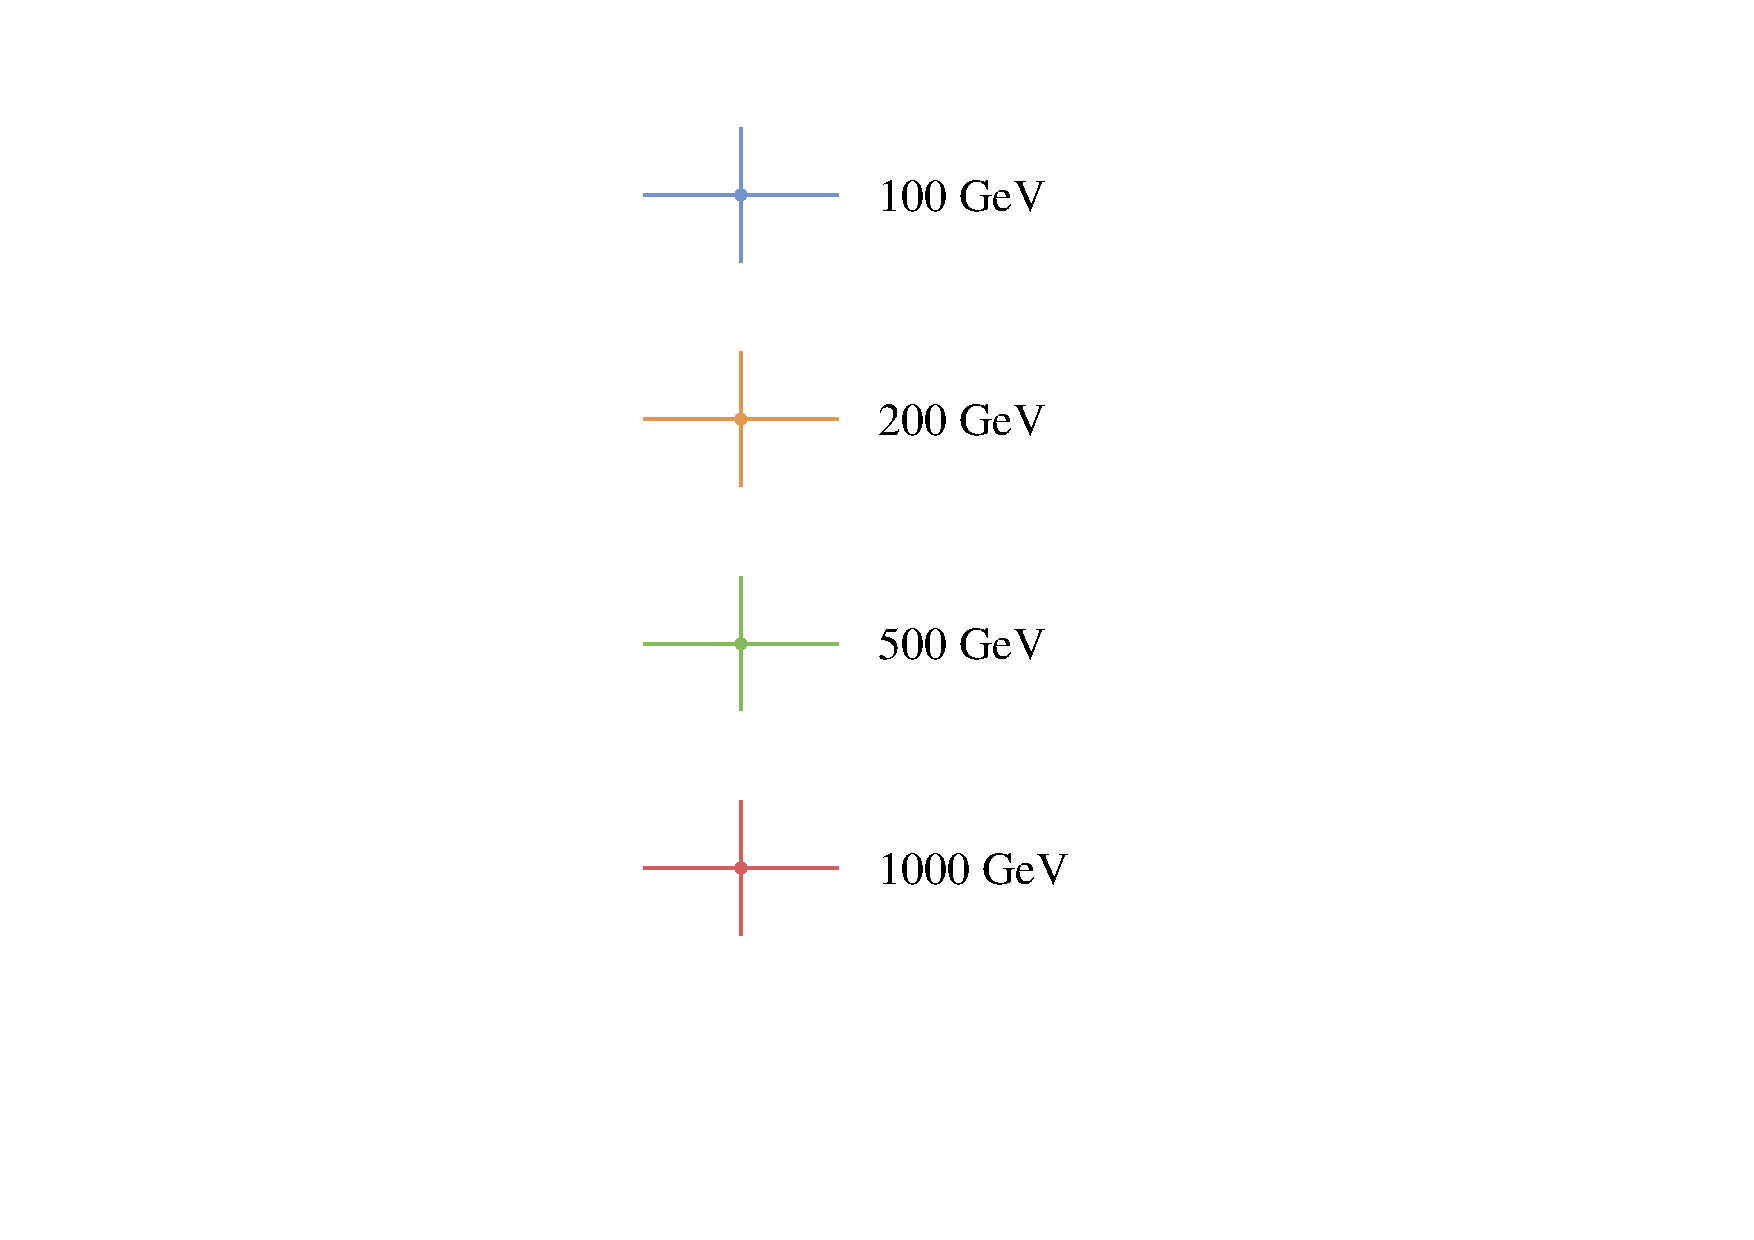
\includegraphics[width=\textwidth]{tau/plots3/legend.pdf}
  \caption{}
  \label{fig:tauDecayLegend}
\end{subfigure}
\caption[The correct classification efficiency for  tau hadronic decay final states  as a function of the \ECAL square cell sizes]
{ The correct classification efficiencies as a function of the \ECAL square cell sizes for a) \decayPionShort decay mode; b) \decayRhoShortest decay mode; c) \decayAiPhotonShortest decay mode; d) \decayAiPionShortest decay mode; and e) \decayThreePionPhotonShort decay mode. The legend is shown in f). All plots are produced with  the \ILD detector model using \eeTauTau channel at \sqrtS = 100, 200, 500, and 1000\,GeV.}
\label{fig:TauPionEfficiency}
\end{figure}


\subsection{Tau hadronic decay correct classification efficiency}

There are two reasons to construct a single parameter for  the overall tau hadronic decay efficiency: firstly the multivariate classifier is trained to achieve a best overall classification efficiency; secondly it is easier to compare the impact of different detector models and different centre-of-mass energies on the classification with a single parameter.

The constructed tau hadronic decay correct classification efficiency, \tauHad, is a weighted average correct classification efficiency over five hadronic decay modes:
\begin{equation}
\tauHad = \frac{\sum_{i}^5 {Br}_{i}\varepsilon_{i}}{\sum_{i}^5 {Br}_{i}}  \,,
\label{eq:had}
\end{equation}
where $Br_{i}$ is the branching fraction of the tau  hadronic decay mode $i$; $\varepsilon_{i}$ is the correct reconstruction efficiency of the tau decay mode $i$, defined in \Equation{eqn:tauEff}; and index $i$ is summed over five tau hadronic decay modes: , \decayPionShort; \decayRhoShortest; \decayAiPhotonShortest; \decayAiPionShortest; and \decayThreePionPhotonShort decay modes.

\FIGURE{fig:TauHadronicEfficiency} shows \tauHad as a function of \ECAL cell sizes with different centre-of-mass energies. The \tauHad  decreases with the increase of centre-of-mass energies and the increase of \ECAL cell sizes, because it is increasingly difficult to reconstruct boosted photons with lower \ECAL transverse spatial resolutions.

%The general trend for t
%As the \sqrtS increases, tau decay products are boosted and it is challenging to separate identical decay products. Similarly,  increasing \ECAL cell sizes makes particle separation more difficult.

At a centre-of-mass energy of 100\,GeV, the \tauHad decreases from 94\% at 3\,mm \ECAL cell size, to 91\% at 20\,mm \ECAL cell size. The decrease in \tauHad is approximately linear to the increase in the cell size. The decrease in the \tauHad is greater at a centre-of-mass energy of 200\,GeV, where the \tauHad declines from 94\% at 3\,mm cell size, to 86\% for a  cell size of  20\,mm. The most significant degradation in the \tauHad occurs at  a centre-of-mass energy of 500\,GeV, where the \tauHad decreases from 92\% at 3\,mm cell size, to 78\% at 20\,mm cell size. At a centre-of-mass energy of 1000\,GeV, the \tauHad drops from 85\% at 3\,mm cell size, to 75\% at 20\,mm cell size.

%From 10\,mm cell size onwards, the \tauHad decrease slows down.

The increase in \ECAL cell sizes has a larger impact on the performance of the tau decay classification at high centre-of-mass energies. When the cell size is increased from 3\,mm to 20\,mm, the degradation of \tauHad is greater at \rootSGeV{500} and 1000\,GeV, than the degradation  of \tauHad at \rootSGeV{100} and 200\,GeV. With decay products being spatially close at high centre-of-mass energies, it is more beneficial to have a small \ECAL cell size to reconstruct individual particles.

\begin{figure}[htbp]
\centering % \begin{center}/\end{center} takes some additional vertical space
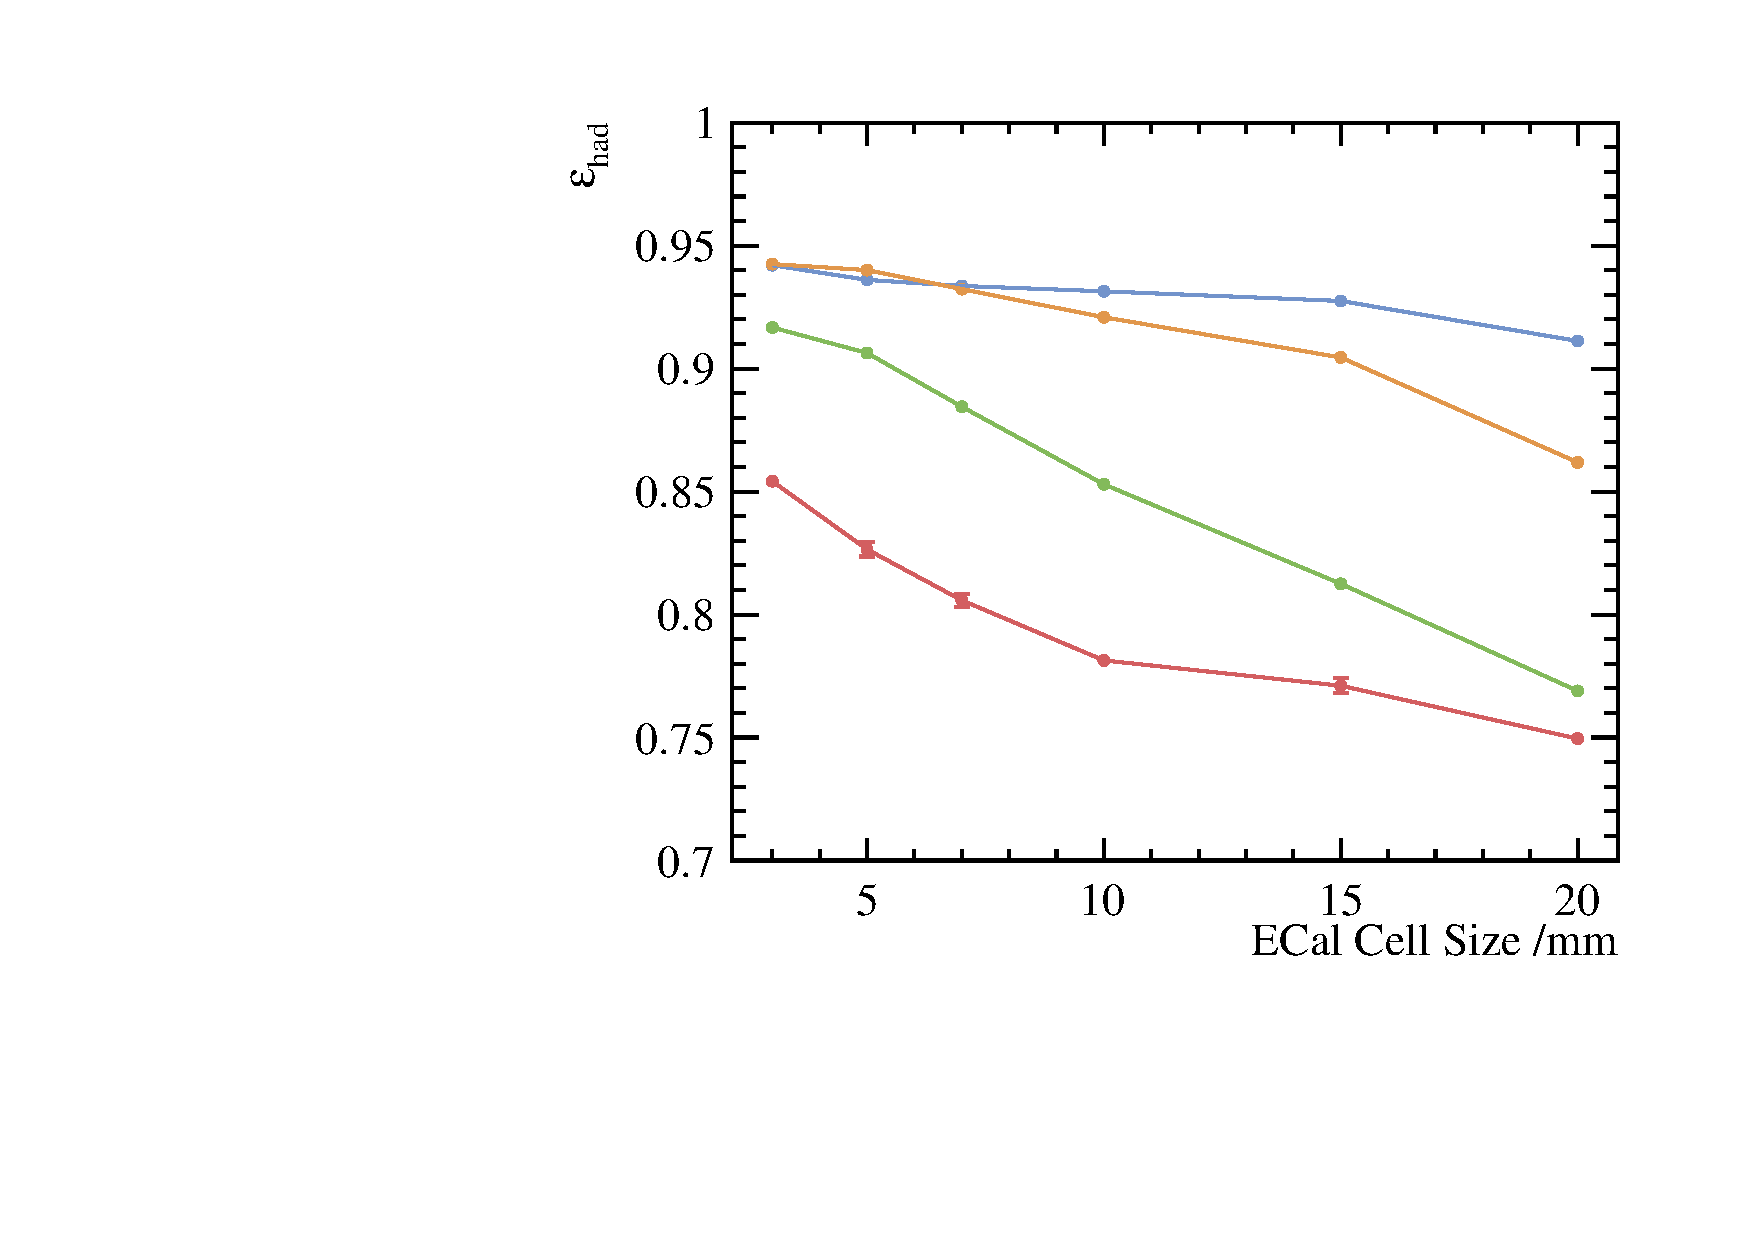
\includegraphics[width=.85\textwidth]{tau/plots3/hadronicEff.pdf}
\caption[The tau hadronic decay efficiency as a function of  the \ECAL cell sizes at different \sqrtS with the \ILD detector model.]
{The tau hadronic decay efficiency, \tauHad, as a function of  the \ECAL cell sizes with different centre-of-mass energies, using \eeTauTau channel simulated with the \ILD detector model. The blue, orange, green, and red lines  represent the \tauHad at \sqrtS = 100, 200, 500 and 1000\,GeV, respectively.}
\label{fig:TauHadronicEfficiency}
\end{figure}


\section{Tau pair polarisation correlations as a signature of Higgs boson}
\label{sec:tauHZ}



A  spin-0 scalar Higgs boson can decay to \TauTauSub{L}{L} or \TauTauSub{R}{R}, whereas  a   spin-1 vector boson \PZ with can decay to \TauTauSub{L}{R} or \TauTauSub{R}{L}, where L, R denotes the tau lepton helicity, due to the helicity conservation. Therefore, by studying the tau pair polarisation correlation from a boson decay, one can determine statistically if the parent boson is a  scalar or a vector.

This section follows the theoretical discussion in \Section{sec:theoryTauPair} on using the correlation between the polarisations of the tau pair from a boson decay as a signature to differentiate the Higgs boson from the \PZ boson. A proof-of-principle analysis  is performed to reconstruct the polarisation correlation of the tau pair with \ZToTauTau channel, where both \tauToPion. The analysis starts with the event generation and simulation, followed by identifying the tau decay products in the events. Afterwards, the tau decay mode classification is used to identify \tauToPion decays. Lastly the tau pair polarisation correlation is presented and compared to  the tau pair polarisation correlation obtained with generator-level Monte Carlo particles.


%For many theories beyond the Standard Model, a common feature is that the coupling of the Higgs particle to leptons increases with the increase of the lepton mass \cite{Duperrin:2008in}.  In these BSM theories, unlike vector bosons coupling to all flavours of leptons equally, the \HigssTauTau coupling would dominate the Higgs coupling to leptons. Therefore, if an experiment observes the breaking of the lepton universality by favouring \TauTau events, it could indicate the existence of a scalar Higgs. When such a universality breaking is observed, a helicity correlation test can be used to show that the \TauTau pair is from a scalar boson or a vector boson. In particular, the polarisation correlations of tau leptons are different for \HiggsToTauTau and \ZToTauTau, as scalar Higgs decays to \TauTauSub{L}{L} or \TauTauSub{R}{R} and \PZ decays to \TauTauSub{L}{R} or \TauTauSub{R}{L}, where L, R denotes the tau lepton helicities.


%Tau pair polarisation correlations can be studied using various tay decay modes. Here \Reference{Bullock:1991my} is followed and the \tauToPion decay mode is used as the example. The Higgs and \PZ boson decay to a  tau pair, where both tau leptons subsequently decay   via  \tauToPion, can be represented as:



%Many BSM theories predict the \HigssTauTau coupling would dominate the Higgs boson to leptons couplings  \cite{Duperrin:2008in}. Therefore, if an experiment observes an excess of tau pair decay events, it could be an indication of the Higgs boson. Here, this section follows


%Comparing \HiggsToTauTau  and \ZToTauTau, the difference in the spin of the bosons reflects in the different polarisation correlation of the tau pair. By extracting the polarisation correlations of the tau pair, the parent boson can be identified.

%The subsequent sections discuss the ability to reconstruct the polarisation correlation of the tau pair with \ZToTauTau channel, where both \tauToPion. The analysis starts with the event pre-selection, followed by identifying the tau decay products in the events. Afterwards, the tau decay mode classification is used to identify \tauToPion decays. Lastly the tau pair polarisation correlation is presented and compared to the correlation distribution obtained with Monte Carlo simulation.

\subsection{Event generation and simulation}

The studied process  is \HepProcess{\Pep \Pem \to \PZ \PZ}, where one \PZ boson decays hadronically and the other \PZ boson decays to a tau lepton pair. The samples were generated at a centre-of-mass energy of 350\,GeV without \ISR contribution for this proof-of-principle study.

The same seven tau decay modes defined in the previous analysis in \Section{sec:tauDecayModes} are studied. The constraints on the simulated events are the same as those   in the previous analysis in \Section{sec:tauSim}, except that the constraint on the total energy of non-neutrino decay products is not applied. A considerable fraction of \ZToTauTau events, where \tauToPion, have two low-energy charged pions. Therefore, the constraint on the total energy of non-neutrino decay products would distort the energy distribution of the charged pions, thus affecting the tau pair polarisation correlation extration.

 %The \tauToPion decay mode is selected for the proof-of-principle analysis of \PHiggs/\PZ separation with tau pair decay channel.

\subsection{Find tau decay products}
\label{sec:tauHZfindTau}

The final state of the process, \eeZZQQ, contains two tau leptons and two quark jets. Therefore, tau decay products can either be found by direct tau lepton decay products searching with a tau finder processor, or by using jet algorithms to find tau decay products as jets. When a tau lepton decays to a few particles, such as the leptonic tau decay final states, the direct tau searching method is favoured. When a tau lepton decays hadronically, resulting in multiple charged and neutral particles, the jet cluster method is suitable to find tau decay methods. Hence, two approaches are combined to find the two tau leptons decay products.

%If a tau lepton decays into a few particles, then the direct tau searching would work better. If a tau lepton decays into many particles, finding tau decay products as jets has a better performance, as jet clustering works better with more particles.

\subsubsection{Direct tau searching}

Tau finder processer, \BonoTauFinder, is a modified version of the one used in the double Higgs analysis in \Section{sec:doubleHiggsBonoTauFinder}. The idea is to find tau decay products consistent with tau decay topologies, and to require the tau  decay products to be isolated from the rest of the particles.

%Parameters chosen are set to find as many tau candidates as possible.

%The filtering of the candidates is via kinematic constraints.

\TABLE{tab:tauBonoTauFinderProcessor} lists all the cuts used in the \BonoTauFinder. Particles with transverse momentum (\pT) less than 0.5\,GeV are not considered. A seed particle is chosen and a search cone is formed around the seed, which requires one or three tracks with the invariant mass  of all particles inside the search cone ($m_{c}$) less than 3\,GeV. Particles are iteratively added to the search cone with a gradually widening opening angle of the search cone. The maximum search cone opening angle ($\theta_S$) is $\cos^{-1}(0.99)$. The isolation criteria states that the opening angle between the search cone  and the $2^{nd}$ closest charged particle ($\theta_{c-2^{nd}X^+}$) is larger than 0.6\,rad. If the criteria is satisfied,  particles associated with the search cone  is identified are the decay products of one tau lepton.


\begin{table}[!htbp]
\begin{tabular}{lr}
\hline
\hline
Modified \BonoTauFinder  & Selection \\
\hline
Veto low \pT &  $\pT < 0.5$\,GeV\\
Seed particle & $\pT > 1$\,GeV \\
Maximum search cone opening angle  & $\theta_S \leqslant \cos^{-1}(0.99)$\\
Tau candidate rejection & $N_{X^+} \neq$ 1 or 3; $m_{c} > 3$\,GeV   \\
Isolation & $\theta_{c-2^{nd}X^+} > 0.6$\,rad\\
\hline
\hline
\end{tabular}
\caption
{Optimised parameters for the modified \BonoTauFinder.}
\label{tab:tauBonoTauFinderProcessor}
\end{table}

\subsubsection{Jet clustering}

Tau hadronically decay products can be also identified as a small jet. The Durham algorithm  (see \Section{sec:pandoraJetDurham}) was used to form  jets. The jet algorithm runs in the exclusive mode to find four jets for \eeZZQQ events.

%Two jets correspond to two quark jets and the other two jets correspond to two tau lepton decay products.

\subsubsection{Selecting best tau candidates for each tau finding method}

The direct tau searching method may find more than two tau  candidates, where each tau candidate corresponds to one tau lepton decay products. To identified the best two tau candidates, kinematic constraints are used.  For example, in  \HepProcess{\Pep \Pem \to \PZ \PZ} events, the energy of the \PZ boson is half of the centre-of-mass energy. The invariant mass of two quarks from \PZ should be close to \PZ mass. Therefore, the $\chi^2$ minimisation function utilising kinematic constraints is:
\begin{equation}
\chi^2 = \frac{\parenths{m_{\Pquark\Pquark} - m_{\PZ}}^2}{\sigma_{m_{\Pquark\Pquark}}^2} + \frac{\parenths{E_{\Pquark\Pquark} - \frac{\sqrtS}{2}}^2}{\sigma_{E_{\Pquark\Pquark}}^2},
\label{eq:tauMinimiser}
\end{equation}
where \sqrtS is the centre-of-mass energy; the variable $m_{\PZ}$ is the mass of \PZ boson from reference \cite{Agashe:2014kda}; the variables $\sigma_{m_{\Pquark\Pquark}}$ and $\sigma_{E_{\Pquark\Pquark}}$ are the reconstructed mass resolution  and energy resolution of the \ZToqq, respectively;  the variables $m_{\Pquark\Pquark}$ and  $E_{\Pquark\Pquark}$ are obtained from the recoil momenta against two tau candidates, assuming that the collision occurs at \sqrtS. The  $m_{\Pquark\Pquark}$ is defined as the invariant mass of the recoil momenta, and  the $E_{\Pquark\Pquark}$ is defined as the energy of the recoil momenta.; and the minimisation is iterated over all tau candidates.

This minimisation produces two best tau candidates for the direct tau searching method. For the jet clustering method, to find the two jets corresponding to two tau lepton decay, the same $\chi^2$ minimisation function is used.  The variables $m_{\Pquark\Pquark}$ and  $E_{\Pquark\Pquark}$ are defined as the total invariant mass and energy of two non-tau-candidate jets, respectively. All other variables in the minimisation function are defined in the same way. After applying the minimisation function, two jets will be identified as the best two tau candidates from the jet clustering method.


%Each of the above two methods produces potentially more than two tau candidates. For example, the direct tau searching method may find many tau candidates

\begin{comment}
Each tau candidate corresponds to one tau lepton decay products from the direct tau searching method, or one jet from the jet clustering method. To identified the best two tau candidates within a method, kinematic constraints are used.  For example, in  \HepProcess{\Pep \Pem \to \PZ \PZ} events, the energy of the \PZ boson is half of the centre-of-mass energy. The invariant mass of two quarks from \PZ should be close to \PZ mass. Therefore, the $\chi^2$ minimisation function utilising kinematic constraints is:
\begin{equation}
\chi^2 = \frac{\parenths{m_{\Pquark\Pquark} - m_{\PZ}}^2}{\sigma_{m_{\Pquark\Pquark}}^2} + \frac{\parenths{E_{\Pquark\Pquark} - \frac{\sqrtS}{2}}^2}{\sigma_{E_{\Pquark\Pquark}}^2},
\label{eq:tauMinimiser}
\end{equation}
where \sqrtS is the centre-of-mass energy; the variable $m_{\PZ}$ is the mass of \PZ boson from reference \cite{Agashe:2014kda}; the variables $\sigma_{m_{\Pquark\Pquark}}$ and $\sigma_{E_{\Pquark\Pquark}}$ are the reconstructed mass resolution  and energy resolution of the \ZToqq, respectively;  the variables $m_{\Pquark\Pquark}$ and  $E_{\Pquark\Pquark}$ are defined differently for the direct tau searching and the jet clustering methods; and the minimisation is iterated over all tau candidates  from direct tau searching method or over all jets from jet clustering method.

For the direct tau searching method, $m_{\Pquark\Pquark}$ and  $E_{\Pquark\Pquark}$ are obtained from the recoil momenta against two tau candidates, assuming that the collision occurs at \sqrtS. The  $m_{\Pquark\Pquark}$ is defined as the invariant mass of the recoil momenta, and  the $E_{\Pquark\Pquark}$ is defined as the energy of the recoil momenta. For the jet clustering method,  $m_{\Pquark\Pquark}$ and  $E_{\Pquark\Pquark}$ are defined as the total invariant mass and energy of two non-tau-candidate jets, respectively.

The $\chi^2$ minimisation function is repeated for the direct tau searching method and the jet clustering method. For each method, the minimisation produces a best pair of  tau candidates with the smallest $\chi^2$.
\end{comment}

\subsubsection{Selecting best tau candidates in an event}

Having identified the best two tau candidates for each method, a set of conditions is used to determine the best overall pair of  tau candidates in an event. If the best pairs of tau  candidates from both methods satisfy the kinematic constraint:
\begin{equation}
\absOf{m_{\Pquark\Pquark} - m_{\PZ}} < \sigma_{m_{\Pquark\Pquark}},\quad \absOf{E_{\Pquark\Pquark} - \frac{\sqrtS}{2}} < \sigma_{E_{\Pquark\Pquark}},
\label{eq:tauMinimiserSelector}
\end{equation}
the pair of  tau  candidates  with smallest $\chi^2$ is selected as the best pair of tau  candidates. Otherwise, if only one pair of tau candidates satisfies the constraint in \Equation{eq:tauMinimiserSelector}, that pair is chosen. If none of the pairs satisfies the constraint, and if one jet from the jet clustering is close to the beam pipe and there are exactly two tau candidates obtained from \BonoTauFinder, then these two tau candidates from \BonoTauFinder  are chosen. This is because if one jet is close to the beam pipe, it is likely that some particles close to the beam pipe are undetected, which leads to a failure in the kinematic constraint and/or the jet reconstruction. Lastly, if all conditions above are not satisfied, two smallest jets by the number of \PFOs from the jet clustering method are chosen to be the best pair of tau  candidates.

\subsection{Boosting tau decay products}

%The previous section describes the method to identify the tau pair decay products.

To use the tau decay mode classifier, it is necessary to know the tau lepton energy to calculate the variables used in the classifier. For the channel \HepProcess{\PZ \to \APtauon \Ptauon}, the  energy of the tau lepton can be obtained in \ZToTauTau decay rest frame, which is half of the \PZ boson energy in the \ZToTauTau rest frame. Hence the tau decay products need to be boosted to the \ZToTauTau decay rest frame for the calculation of the variables used in the MVA classification.

%The boosting requires the \fourMomentum of the \PZ.

The boosting of the tau decay product requires the \fourMomentum of the Z boson, where \ZToTauTau, which is calculated from the recoil momenta of non tau-decay-products:
\begin{equation}
p^{\mu}_{\Ptau\Ptau} =
  \begin{pmatrix}
    \sqrtS\\   \sqrtS\times\sin\parenths{\theta_{beam}}\\  0   \\       0 \\
  \end{pmatrix}
  - \sum_{i}^{non-\Ptau}p^{\mu}_{i},
\end{equation}
where $\theta_{beam}$ is the beam crossing angle; \sqrtS is the centre-of-mass energy; $p^{\mu}_{i}$ is the four-momentum vector of the particle $i$; $p^{\mu}_{\Ptau\Ptau}$ is the four-momentum vector of the \PZ, where \ZToTauTau; and  index $i$ is summed over all non-tau-decay-product \PFOs. Extra kinematic constraint fixes the energy of the \PZ boson to be a half of \sqrtS:
\begin{equation}
p^{\mu}_{\Ptau\Ptau,correct} = p^{\mu}_{\Ptau\Ptau} \times \frac{\frac{1}{2}\sqrtS}{E_{\Ptau\Ptau}},
\end{equation}
where $E_{\Ptau\Ptau}$ is the energy of the vector $p^{\mu}_{\Ptau\Ptau}$  and other variables are defined in the same way as in the previous equation. The vector $p^{\mu}_{\Ptau\Ptau,correct} $ is then treated as the four-momentum vector of \PZ boson, where \ZToTauTau. Tau decay products are boosted to the \PZ decay rest frame accordingly. The calculation of the variables used in the MVA classifier are then performed in the \ZToTauTau decay rest frame.

\subsection{Variables used in the MVA}

Variables used in  the MVA classifier are a subset of the ones listed in \Table{tab:tauVaraibles}. Variables regarding EM shower profiles, calorimeter hit information, and track information are not used (the last three rows in \Table{tab:tauVaraibles}) as the information was not available in the outputs of the standard version of \pandora used in this analysis.

%Also for the computational reason, it was not feasible to use these variables for the MVA. \Pep and \Ppiplus separation could be improved if these extra variables are included.


\subsection{Multivariate analysis}

The training  the multivariate classifier follows the procedure in  \Section{sec:tauMVA}. The same classifier with the same parameters as in the previous tau decay mode classification  is used.   In the tau decay mode classifier applying stage, \tauToPion decay mode is selected with an additional criteria that there is at least one charged pion among the tau decay products.

\subsection{Result}

\FIGURE{fig:TauSpin2D} shows the two-dimensional distributions of  tau decay product energy fractions, with \eeZZ channel where one \PZ decays to a tau pair and the other \PZ decays hadronically, using both \tauToPion decay mode. The energy fractions of the tau decay product to the tau lepton ($E_{\Ppiplus} / E_{\APtauon}$ and $E_{\Ppiminus} / E_{\Ptauon}$) are the appropriate kinematic variables to study the tau pair polarisation correlation, motivated in the theoretical discussion in \Section{sec:theoryTauPair}.

\FIGURE{fig:TauSpin2DMC} shows the  two-dimensional  tau decay product energy fraction distribution obtained with the generator-level  Monte Carlo particles. \FIGURE{fig:TauSpin2Dreco} shows the distribution using the full detector simulation. A good match between the distributions obtained with  the generator-level  MC particles and the full detector simulation is achieved. Dark regions along the diagonal can be seen in both the distribution for the Monte Carlo particles and the distribution for the full detector simulation. In the \ZToTauTau decays, where both \tauToPion, an energetic \Pgppm is likely to be associated with an energetic \Pgpmp and a low-energy \Pgppm is  likely to be associated with a low-energy \Pgpmp. Comparing the two figures, some events in the top right quadrant, corresponding to  both \Ppipm being energetic, are not reconstructed correctly in the full detector simulation. This is due to the incorrect finding of the tau pair decay products  in \Section{sec:tauHZfindTau}.


% This trend is shown in both the distribution produced with the Monte Carlo particles and with the full detector simulation

This proof-of-principle analysis shows the tau polarisation correlations, using the \eeZZ channel where one \PZ decays hadronically and the other \PZ decays to a tau pair and subsequently both \tauToPion,  is possible to be observed with the \ILD detector model at \rootSGeV{350}. With a similar study of the \eeHZ channel where \PH decays hadronically and \PZ decays to a tau pair and both \tauToPion,  the  tau pair decay products energy distribution can be used to statistically identify if the parent boson is a Higgs boson or a \PZ boson.

%, and to identify Higgs boson in an experiment that observes the breaking of the lepton universality by favouring tau pair events.


%If the tau pair decay from Higgs boson is observed, the decay can be recognised in the \tauToPion mode as a high-energy \Pgppm with a low-energy \Pgpmp. Hence, the tau decay product energy distribution can be a clean signature for \HiggsToTauTau.

%\FIGURE{fig:theoryTauPairCorrelation} shows the resulting two-dimensional distributions of  $\overline{z} = \frac{E_{\Ppiplus}}{E_{\APtauon}}$ versus  $z = \frac{E_{\Ppiminus}}{E_{\Ptauon}}$ for \ZToTauTau and \HiggsToTauTau channels, where both tau leptons decay via \tauToPion. The difference of the tau pair polarisation correlation between \PZ and \PHiggs  is clear. The energy distribution of the charged pion from \ZToTauTau has the form of $\overline{z}  \sim z$, whilst the distribution from  \HiggsToTauTau has the form of $\overline{z}  \sim (1-z)$. Therefore, in \ZToTauTau process, a high-energy \Pgppm  is likely to be associated with a high-energy \Pgpmp. In \HiggsToTauTau process, the opposite is favoured. If the tau pair decay from Higgs boson is observed, the decay can be recognised in the \tauToPion mode as a high-energy \Pgppm with a low-energy \Pgpmp. Hence, the tau decay product energy distribution can be a clean signature for \HiggsToTauTau.


\begin{figure}[htbp]
\centering % \begin{center}/\end{center} takes some additional vertical space
\begin{subfigure}[b]{0.75\textwidth}
  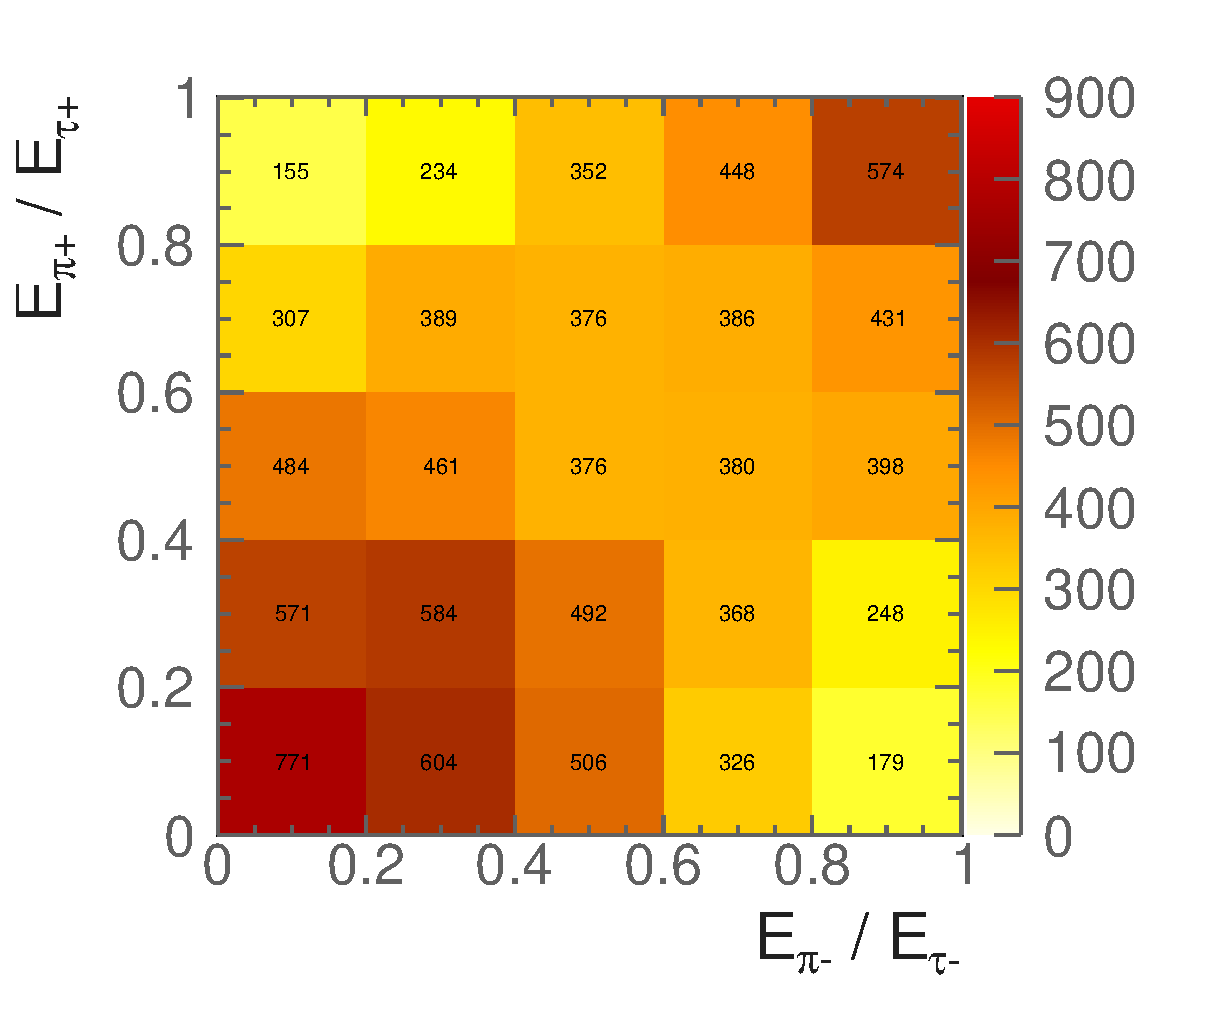
\includegraphics[width=\textwidth]{tau/NoTimeAnalysis/2DMC}
  \caption{Generator-level  Monte Carlo particles}
  \label{fig:TauSpin2DMC}
\end{subfigure}
\begin{subfigure}[b]{0.75\textwidth}
  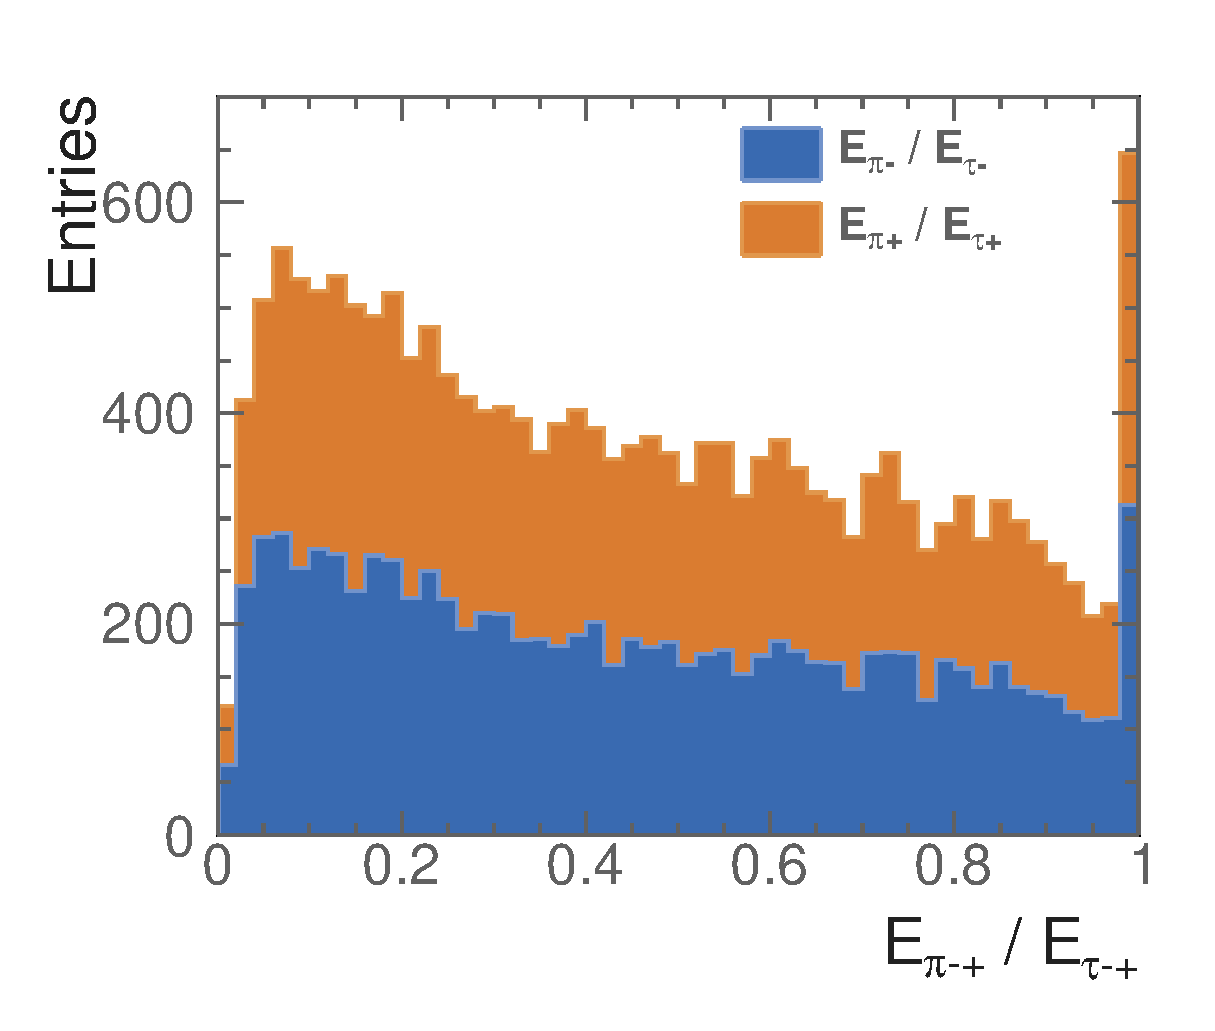
\includegraphics[width=\textwidth]{tau/NoTimeAnalysis/2Dreco}
  \caption{Full detector simulation}
  \label{fig:TauSpin2Dreco}
\end{subfigure}
\caption
{Two-dimensional distributions of $E_{\Ppiplus}/E_{\APtauon}$ as a function of $E_{\Ppiminus}/E_{\Ptauon}$ from \ZToTauTau decay where both \tauToPion, with \eeZZ channel where one \PZ decays to a tau pair and the other \PZ decays hadronically,  for a) generator-level  Monte Carlo particles, and b) the full detector simulation. The \tauToPion decay is selected using a) the truth information, and b) the MVA classifier.}
\label{fig:TauSpin2D}
\end{figure}
\begin{comment}
\begin{figure}[htbp]
\centering % \begin{center}/\end{center} takes some additional vertical space
\begin{subfigure}[b]{0.45\textwidth}
  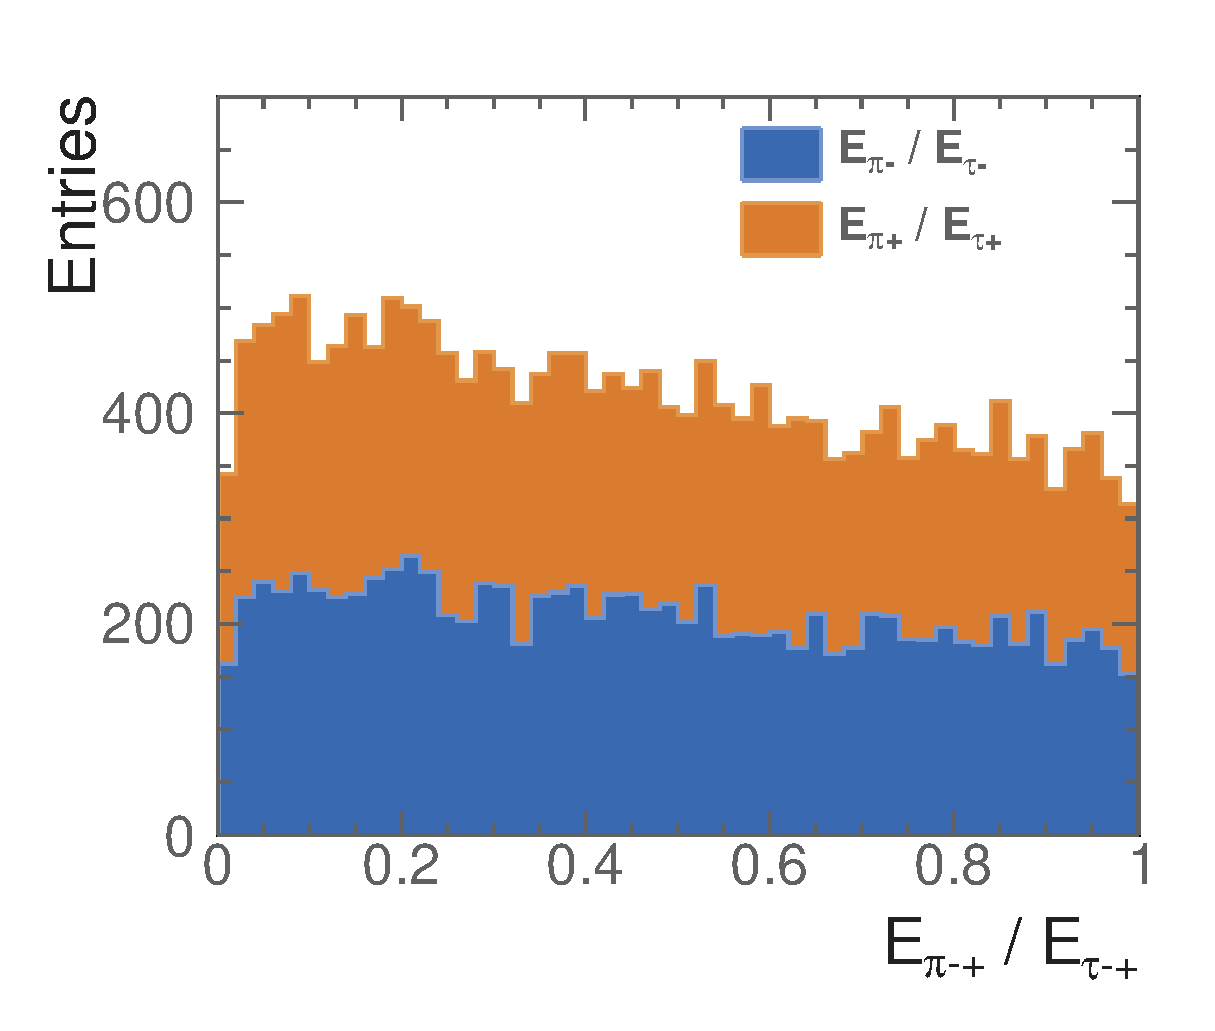
\includegraphics[width=\textwidth]{tau/NoTimeAnalysis/1DMC}
  \caption{Truth info.}
  \label{fig:TauSpin1DMC}
\end{subfigure}
\begin{subfigure}[b]{0.45\textwidth}
  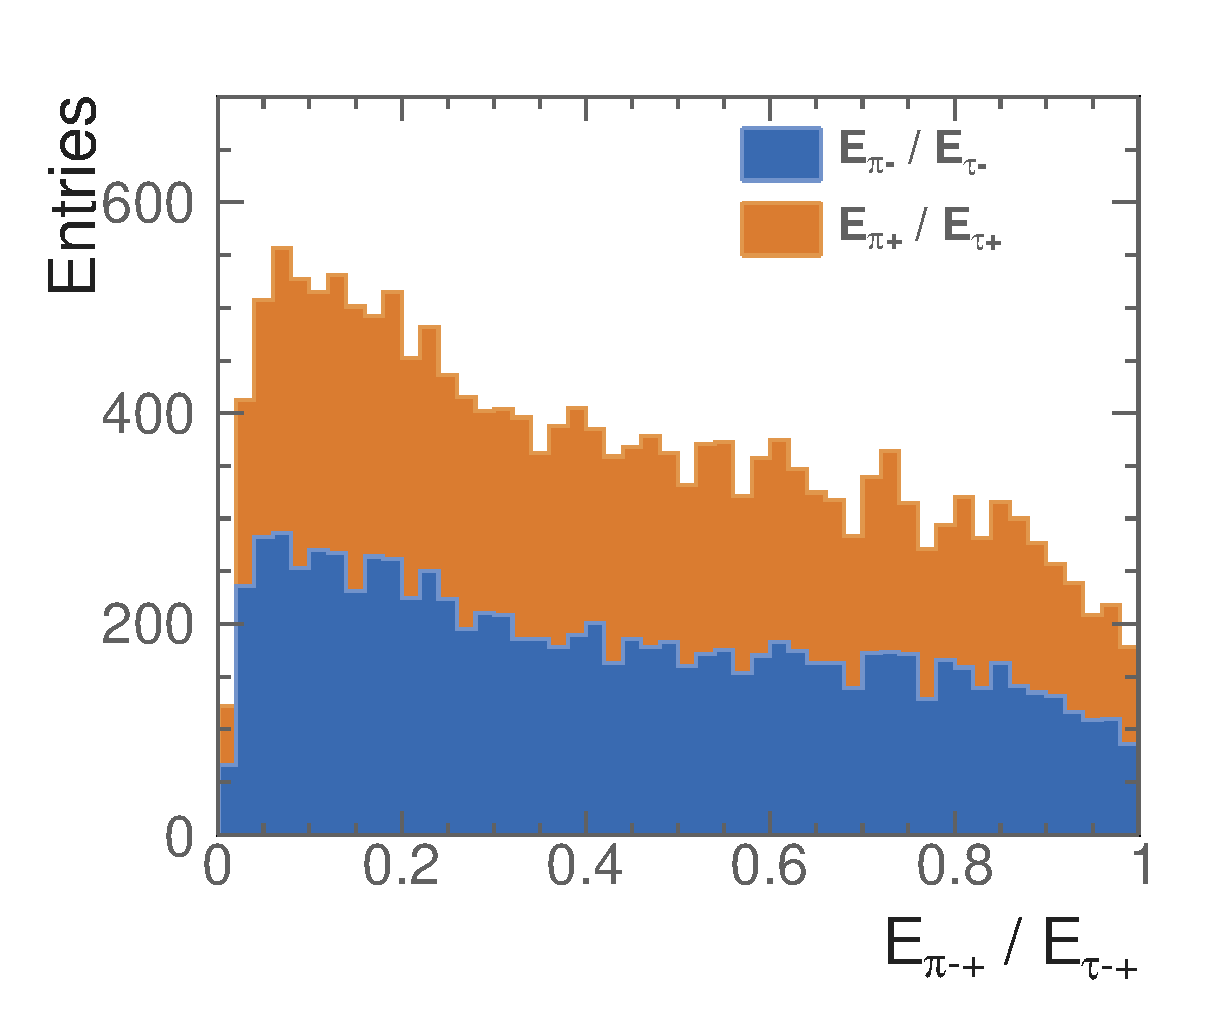
\includegraphics[width=\textwidth]{tau/NoTimeAnalysis/1DrecoNoOverflow}
  \caption{Reconstructed}
  \label{fig:TauSpin1Dreco}
\end{subfigure}
\caption[One-dimensional plot of spin correlations of the tau lepton pair from \PZ decay, using \decayPionShort decay mode.]
{One-dimensional plot of spin correlations of the tau lepton pair from \PZ decay, using \decayPionShort decay mode.}
\label{fig:TauSpin1D}
\end{figure}

\end{comment} 